%% Latex template for PhD dissertation or MS thesis
%% Electrical and Computer Engineering Department
%% Brigham Young University
%% Last Modified:  March 2012

\documentclass[12pt]{report}

%%%%%%%%%%%%%%%%%%%%%%%%%%%%%%%%%%%%%%%%%%%%%%%%%%%%%%%%
%  Setup BYU thesis format
%%%%%%%%%%%%%%%%%%%%%%%%%%%%%%%%%%%%%%%%%%%%%%%%%%%%%%%%
\usepackage{amsmath}
\usepackage{mathrsfs,amsmath}
\interdisplaylinepenalty=2500
\usepackage{cite}
\usepackage{dcolumn}
\usepackage{times}
\usepackage{fancyhdr}
\usepackage{setspace}

\usepackage{latexsym} % Need this for \Box
\usepackage{graphicx}
\usepackage{rotating}
%\usepackage[pdftex]{graphicx}
\usepackage{epstopdf}

\usepackage{byustyle}
\usepackage{epstopdf}
\usepackage{booktabs}
\usepackage{nicefrac}
\usepackage{mathtools}
\usepackage{listings}
\usepackage{xcolor}
% source code listing
\newcommand{\axpy}{{\ttfamily axpy}\xspace}
\newcommand{\extra}{{\bfseries extra}:\xspace}
%\newcommand{\lst}[1]{\colorbox{white!90!blue}{\lstinline!#1!}}
\newcommand{\lst}[1]{\colorbox{white!20!black}{\lstinline!#1!}}
\newcommand{\lstfont}[1]{\color{#1}\scriptsize\ttfamily}
\newcommand{\lsttinyfont}[1]{\color{#1}\fontsize{7}{7}\ttfamily}
\newcommand{\lstinlinefont}[1]{\color{#1}\scriptsize\ttfamily}
\definecolor{mygray}{rgb}{0.97,0.97,0.97}

% set indent to a more reasonable level (so that itemize can be used in columns)
\setlength{\leftmargini}{20pt}


\lstdefinestyle{myCUDAstyle} {
	language=[ANSI]C++,
    showstringspaces=false,
    backgroundcolor=\color{mygray},
    basicstyle=\lstfont{black},
    identifierstyle=\lstfont{black},
    keywordstyle=\lstfont{magenta},
    numberstyle=\lstfont{black},
    stringstyle=\lstfont{cyan},
    commentstyle=\lstfont{yellow!30!black},
    moredelim=[is][\lstfont{green!50!black}]{@}{@},
    emph={
        cudaMalloc, cudaFree,
        cudaMallocHost, cudaFreeHost,
        cudaMemcpyAsync, cudaMemcpy, cudaMemcpyHostToDevice, cudaMemcpyDeviceToHost,
        cudaSuccess, cudaGetLastError, cudaGetErrorString,
        cudaErrorMemoryAllocation, cudaError_t,
        cudaOccupancyMaxPotentialBlockSize,
        __global__, __shared__, __device__, __host__,
        __syncthreads,
        cudaEvent_t, cudaStream_t,
        cudaEventCreate, cudaEventSynchronize, cudaEventDestroy,
        cudaEventElapsedTime, cudaEventQuery, cudaEventRecord,
        cudaStreamWaitEvent,
        threadIdx, blockIdx, blockDim, gridDim,
        cudaStream_t, cudaStreamCreate, cudaStreamDestroy,
        cudaMemcpyDeviceToDevice, cudaMemcpyHostToHost,
    },
    emphstyle={\lstfont{green!50!black}},
    breaklines=true,
    numbers=left
    }
    
    \lstdefinestyle{myCUDAstyle_inline} {
	language=[ANSI]C++,
    showstringspaces=false,
    backgroundcolor=\color{white},
    basicstyle=\lstfont{black},
    identifierstyle=\lstfont{black},
    keywordstyle=\lstfont{magenta},
    stringstyle=\lstfont{cyan},
    commentstyle=\lstfont{yellow!30!black},
    moredelim=[is][\lstfont{green!50!black}]{@}{@},
    emph={
        cudaMalloc, cudaFree,
        cudaMallocHost, cudaFreeHost,
        cudaMemcpyAsync, cudaMemcpy, cudaMemcpyHostToDevice, cudaMemcpyDeviceToHost,
        cudaSuccess, cudaGetLastError, cudaGetErrorString,
        cudaErrorMemoryAllocation, cudaError_t,
        cudaOccupancyMaxPotentialBlockSize,
        __global__, __shared__, __device__, __host__,
        __syncthreads,
        cudaEvent_t, cudaStream_t,
        cudaEventCreate, cudaEventSynchronize, cudaEventDestroy,
        cudaEventElapsedTime, cudaEventQuery, cudaEventRecord,
        cudaStreamWaitEvent,
        threadIdx, blockIdx, blockDim, gridDim,
        cudaStream_t, cudaStreamCreate, cudaStreamDestroy,
        cudaMemcpyDeviceToDevice, cudaMemcpyHostToHost,
    },
    emphstyle={\lstfont{green!50!black}},
    breaklines=true,
    }

\definecolor{codenumber}{rgb}{0.5,0.5,0.5}
\definecolor{codekeyword}{rgb}{0.9,0.4,0.7}
\definecolor{codeCUDA}{rgb}{1.0,0.6,0.6}
%\DeclareTextFontCommand{\emph}{\bfseries\color{blue!70!black}}

\usepackage[numbered,framed]{matlab-prettifier}
\usepackage{filecontents}

% Setup the byu style sheet
\byustylesetup{%
    %
    %isdissertation = true,            % Uncomment this if you're doing a PhD dissertation
    %etdsubmission = true,            % Uncomment this if you're compiling it for ETD submission
    singlepageabstract = true, % Comment this out if your abstract is multiple pages
    singlepageacknowledgements = true, % Uncomment this if your Acknowledgements is multiple pages
    %
    % Definitions of names needed in thesis/dissertation
    deptname          = Department of Electrical and Computer Engineering,    %
    collegename       = Ira A. Fulton College of\\Engineering and Technology, %
    committeechairman = Michael D. Rice,                      %
    committeemembera  = Brian D. Jeffs,                         %
    committeememberb  = Brian A. Mazzeo,                          %
    %committeememberc  = Firstname Mi. Lastname,                    % PhD Only
    %committeememberd  = Firstname Mi. Lastname,                     % PhD Only
    graddate = April 2017,  % Leave commented for current month and year
    %copyrightyear = 2012,      % Leave commented for current year
    % uncomment the keywords for a dissertation
    %keywords         = {elecromagnetic waves, crazy circuits}
    %
    % Uncomment to shorten for proofreading purposes
    %noabstract = true,         % Don't show the abstract page
    %nouniversitypages = true,  % Don't show any of the "university pages"
    %noacknowledgements = true, % Don't show the Acknowledgements page
    %notableofcontents = true,  % Don't show the Table of Contents
    %nolistoffigures = true,    % Don't show the List of Figures
    %nolistoftables = true,     % Don't show the List of Tables
    %notocandlists = true,      % Don't show the Table of Contents, List of Figures, or the List of Tables
    %noheaderatall = true,      % Don't show any of the BYU Thesis header pages
}
%%%%%%%%%%%%%%%%%%%%%%%%%%%%%%%%%%%%%%%%%%%%%%%%%%%%%%%%
%  END:  Setup BYU thesis format
%%%%%%%%%%%%%%%%%%%%%%%%%%%%%%%%%%%%%%%%%%%%%%%%%%%%%%%%%

%%%%%%%%%%%%%%%%%%%%%%%%%%%%%%%%%%%%%%%%%%%%%%%%%%%%%%%%
%  Include other \usepackage{} statements here.
%    Add one package at a time.
%    Warning:  Some packages are not compatible with byuthesis.sty
%%%%%%%%%%%%%%%%%%%%%%%%%%%%%%%%%%%%%%%%%%%%%%%%%%%%%%%%%
%\usepackage[normalmargins]{savetrees} % prints smaller to save trees (draft only)
\usepackage{amsmath,amssymb} % math definitions
\usepackage{graphicx}        % for figures
\usepackage{subfigure}       % for figures with multiple subfigures
\usepackage{setspace}        % so all the captions will be single spaced
%%%%%%%%%%%%%%%%%%%%%%%%%%%%%%%%%%%%%%%%%%%%%%%%%%%%%%%%
%  END: Include other \usepackage{} statements here.
%%%%%%%%%%%%%%%%%%%%%%%%%%%%%%%%%%%%%%%%%%%%%%%%%%%%%%%%%

%%%%%%%%%%%%%%%%%%%%%%%%%%%%%%%%%%%%%%%%%%%%%%%%%%%%%%%%
% For doing bookmarks in the PDF file
%%%%%%%%%%%%%%%%%%%%%%%%%%%%%%%%%%%%%%%%%%%%%%%%%%%%%%%%%
% For more info, see:
% http://www.geocities.com/kijoo2000/latex2pdf.pdf
% http://www.tug.org/applications/hyperref/manual.html
\usepackage[driverfallback=dvipdfm,backref,pagebackref,plainpages=false]{hyperref}
\hypersetup{
    %bookmarks    = true, % Make bookmarks (default=true). This option
                          %cannot be used after package has been loaded,
                          %thus use like this: \usepackage[bookmarks=false]{hyperref}.
    %
    breaklinks   = false, % Allow link text to break across lines (default=false).
    linktocpage  = false, % make page number, not text, be link on TOC, LOF and LOT
    colorlinks   = false, % Color the text of links (true) or put color frames over
                          % the links (false).
% NOTE: if you need to use a dvi->ps->pdf path for things like PSTricks, you
% may find that commenting out the next line is necessary.
    %pdfborder    = 001,   % sets the default for pdf links                      
    pdfstartview = {FitH}, % Set the startup page view. Possible options are:
                           % FitH: Fit whole width of page
                           % FitV: Fit whole height of page
                           % FitB: Fit whole “Bounding Box” page
                           % FitBH: Fit whole width of “Bounding Box” of page
                           % FitBV: Fit whole height of “Bounding Box” of page
    bookmarksnumbered  = true, % Put section numbers in bookmarks (default=false)
    bookmarksopen      = true, % Open up the bookmark trees (default=false).
    bookmarksopenlevel = 1, % Level to which bookmarks are open (default=\maxdimen).
    bookmarkstype      = toc, % Specify which toc file to mimic (default=toc).
    pdfpagemode        = {UseOutlines}, %  Specify how document starts when opened ({None}).
                                        % Possible options are:,
                                        % None: Neither bookmarks nor thumbnails are visible.
                                        % UseOutlines: Bookmarks are visible.
                                        % UseThumbs: Thumbnails are visible.
                                        % FullScreen: Full-screen mode
    pdftitle    = {JeffRavertMastersThesis},
    pdfauthor   = {Jeff Ravert},
    pdfcreator  = {Jeff Ravert},
    pdfsubject  = {Jeff Ravert's Master's Thesis},
    pdfkeywords = {GPU, Equalizer, Estimator, FPGA, BYU},
}
%%%%%%%%%%%%%%%%%%%%%%%%%%%%%%%%%%%%%%%%%%%%%%%%%%%%%%%%
%  END: For doing bookmarks in the PDF file
%%%%%%%%%%%%%%%%%%%%%%%%%%%%%%%%%%%%%%%%%%%%%%%%%%%%%%%%%

%%%%%%%%%%%%%%%%%%%%%%%%%%%%%%%%%%%%%%%%%%%%%%%%%%%%%%%%
%                Macros
%  Define macros here
%%%%%%%%%%%%%%%%%%%%%%%%%%%%%%%%%%%%%%%%%%%%%%%%%%%%%%%%%
\def\proof{\noindent{\it Proof: }}
\def\QED{\mbox{\rule[0pt]{1.5ex}{1.5ex}}}
\def\endproof{\hspace*{\fill}~\QED\par\endtrivlist\unskip}
%
\newcommand{\norm}[1]{\left\|#1\right\|}
\newcommand{\abs}[1]{\left|#1\right|}
\newcommand{\defeq}{\stackrel{\triangle}{=}}
\newcommand{\re}{\mathbb{R}} % real numbers
\newcommand{\OMIT}[1]{{}} % omit sections of text
\newcommand{\pd}[2]{\ensuremath{\frac{\partial #1}{\partial #2}}} % partial derivative
\newcommand{\rpkt}{\mathbf{r}_\text{pkt}}
\newcommand{\Lpkt}{L_\text{pkt}}
\newcommand{\Lp}{L_\text{p}}
\newcommand{\Lasm}{L_\text{ASM}}
\newcommand{\Ldata}{L_\text{d}}

%%%%%%%%%%%%%%%%%%%%%%%%%%%%%%%%%%%%%%%%%%%%%%%%%%%%%%%%%
%                End Macros
%%%%%%%%%%%%%%%%%%%%%%%%%%%%%%%%%%%%%%%%%%%%%%%%%%%%%%%%%

% To only print a few chapters without changing the reference numbers,
% uncomment the chapters you want
%\includeonly{intro}
%\includeonly{chapter2}
%\includeonly{appendixa}

%%%%%%%%%%%%%%%%%%%%%%%%%%%%%%%%%%%%%%%%%%%%%%%%%%%%%%%%%
% Start Document
%%%%%%%%%%%%%%%%%%%%%%%%%%%%%%%%%%%%%%%%%%%%%%%%%%%%%%%%%

\begin{document}

% Define Title & Author
\title{GPU Implementation of Data-Aided Equalizers}
\author{Jeffrey T. Ravert}

% For displaying the BYU Thesis header
% This command assumes that there are documents called abstract.tex and
% acknowledgements.tex that will be included in the header
\showBYUHeader


% Include chapters of the thesis here:
% each chapter should be in a file with a .tex extension and the text
% of the file should begin with \chapter{Chapter Title}, followed
% by the text of the chapter.
%  Note: the introduction is considered Chapter 1.
\chapter{Introduction}
\section{Multipath in Aeronautical Telemetry}
Multipath interference is one of the dominant causes for link loss in aeronautical telemetry.
Strong multipath interference occurs in aeronautical telemetry when the transmitted signal is received from multiple paths because a test article is in a low elevation angle scenario as shown in Figure \ref{fig:multipath}.
Multipath propagation is modeled as linear, time-invariant system with a finite impulse response.
Equalizers have been studied to combat multipath interference in aeronautical telemetry \cite{rice-afran-saquib:2014,rice-afran-saquib-cole-rhodes-moazzami:2014}.

There are two types of equalizers, blind and data-aided.
Blind equalizers combat multipath using known properties of the transmitted signal but no knowledge of the data or multipath channel.
Data-aided equalizers require knowing something about the received signal.
One method of providing data that can be used in data-aided equalization is for the transmitter to periodically insert a known bit sequence called a ``pilot'' into the data stream.
The receiver compares the received signal with a locally stored copy to estimate parameters such as multipath channels, frequency offsets, phase offsets and noise variance.
Data-aided equalizers are finite-length impulse response (FIR) filters. The impulse response of the equalizer filter is computed based on the estimated channel better mitigate multipath.
\begin{figure}
	\centering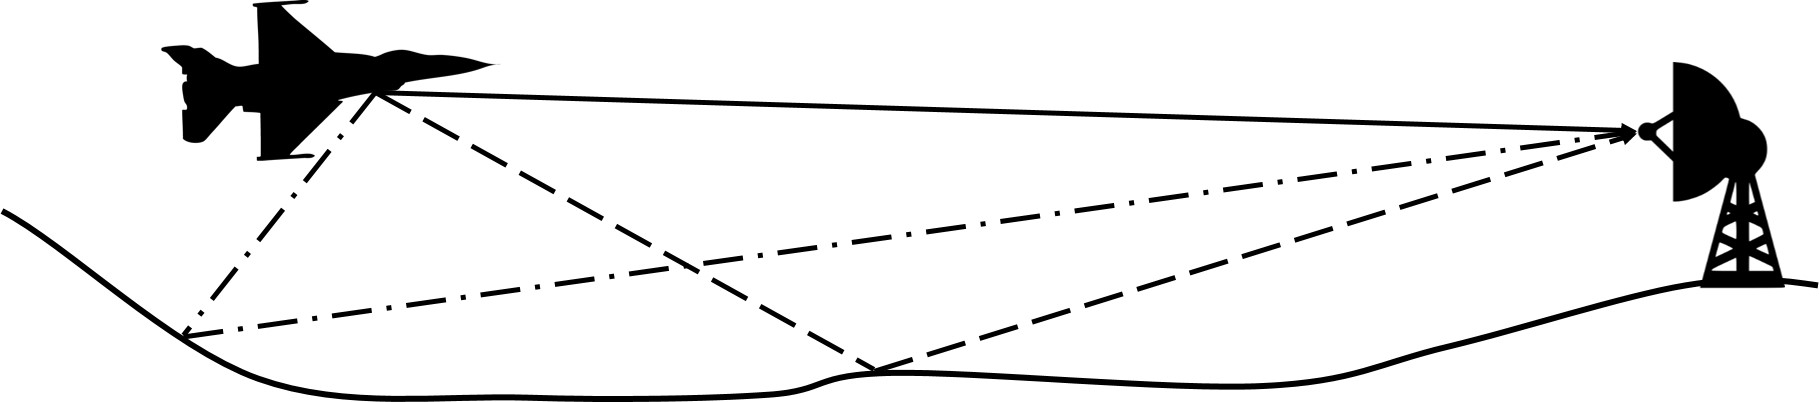
\includegraphics[width=12.11in/100*50]{figures/intro/Picture1.jpg}
	\caption{Multipath can occur when a signal is received multiple paths like line-of-sight or ground bounce or reflections.}
	\label{fig:multipath}
\end{figure}
\section{Problem Statement}
The signal processing for a digital communications system with data-aided equalizers is computationally heavy.
Algorithms implemented in a high powered Central Processing Unit (CPU) can not processing in real-time.
Graphic Processing Units (GPUs) can be used to perform real-time processing because of their massively parallel architecture.

This thesis studies how signal processing can be reformulated to run quickly and efficiently in GPUs.
Processing signals in batches to introduce more parallelism.
Optimized libraries harness GPU resources to make signal processing implementation relatively easy and extremely fast.
If algorithms can be reformulated to used matrix/vector multiplication, solving linear systems of equations, or the Fast Fourier Transform, GPUs can provide vast speed ups.

\section{Organization}
Chapter \ref{chap:equations} shows the equations for these block diagrams.
Chapter \ref{chap:gpu} will shed some light on signal processing in GPUs.
Chapter \ref{chap:equalizers_in_gpus} will illustrate how the five equalizers are implemented in GPUs.
Chapter \ref{chap:final_summary} will summarize.
%%%%%%%%%%%%%%%%%%%%%%%%%%%%%%%%%%%%%%%%%%%%%%%%%%%%%%%%%%%%%%%%%%%%%%%%%%%%%%%%%%%%%%%%%%%%%%
%%%%%%%%%%%%%%%%%%%%%%%%%%%%%%%%%%%%%%%%%%%%%%%%%%%%%%%%%%%%%%%%%%%%%%%%%%%%%%%%%%%%%%%%%%%%%%
%%%%%%%%%%% systemOverview
%%%%%%%%%%%%%%%%%%%%%%%%%%%%%%%%%%%%%%%%%%%%%%%%%%%%%%%%%%%%%%%%%%%%%%%%%%%%%%%%%%%%%%%%%%%%%%
%%%%%%%%%%%%%%%%%%%%%%%%%%%%%%%%%%%%%%%%%%%%%%%%%%%%%%%%%%%%%%%%%%%%%%%%%%%%%%%%%%%%%%%%%%%%%%


% \cleardoublepage
\chapter{Preamble Assisted Equalization Project}
Data-aided equalization in aeronautical telemetry has been studied and tested by the Preamble Assisted Equalization (PAQ) project \cite{paq-phase1-report:2014}.
The PAQ project built a TRL 6 system that compares five data-aided equalizers to blind equalization and no equalization \cite{frerkingjpl}.
Bit error statistics were be used as the figure or merit for the equalization algorithms.
Live flight tests were conducted at Edwards AFB in March and June 2016.
The five data-aided equalizers the PAQ project studied are
\begin{itemize}
\item zero-forcing (ZF) equalizer
\item minimum mean square Error (MMSE) equalizer
\item MMSE initialized constant modulus algorithm (CMA) equalizer
\item frequency domain equalizer one (FDE1)
\item frequency domain equalizer Two (FDE2).
\end{itemize}
\section{Hardware}
\label{sec:hardware}
A block diagram of the PAQ project physical system is shown in Figure \ref{fig:hardwareblock}.
\begin{figure}
	\centering\includegraphics[width=11.58in/100*55]{figures/systemOverview/hardwareblock.pdf}
	\caption{A block diagram of the physical PAQ project hardware. The components inside the rack mounted server are in the dashed box. All the components in the dashed and dotted box are housed in a rack mounted case.}
	\label{fig:hardwareblock}
\end{figure}
A picture of the physical components is shown in Figure \ref{fig:HostSystem}.
\begin{figure}
	\centering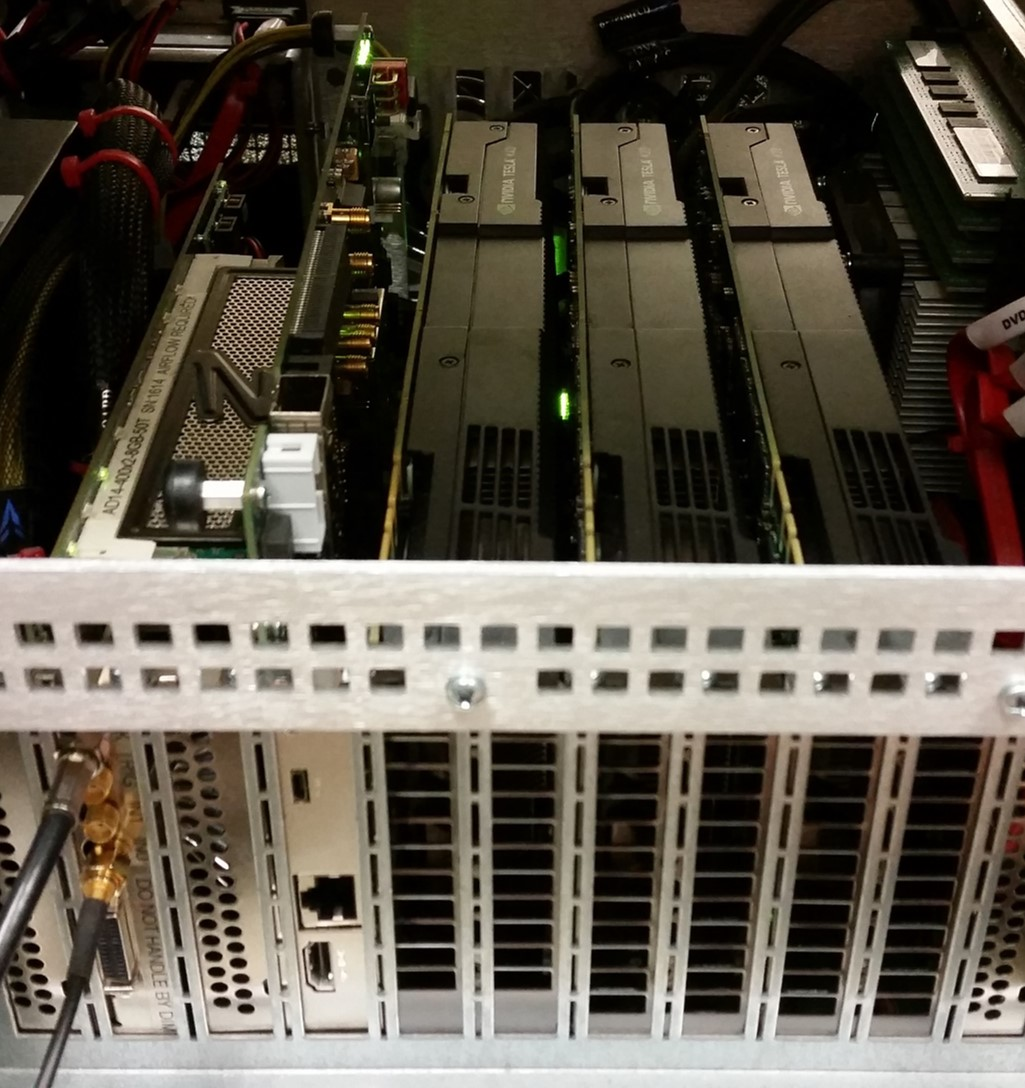
\includegraphics[scale=0.55]{figures/systemOverview/HostSystem.jpg}
	\caption{A picture of the physical PAQ project hardware refrencing blocks from Figure \ref{fig:hardwareblock}. Right: Components in the dashed and dotted box. Left: Components in the dashed box. Note that the T/M Receiver is not pictured.}
	\label{fig:HostSystem}
\end{figure}
The major components, and their functions are summarized in the following.
\begin{itemize}
	\item The \textbf{T/M mixer} down-converts from L or C band RF to IF (70 MHz) then applies an anti-aliasing filter.
	%
	\item The \textbf{rack mounted server} is a high powered computer that houses an ADC, a FPGA and three GPUs 		slotted into a 32 pin PCIe bus.
	\item The \textbf{ADC} produces 14-bit samples of the real-valued bandpass signal
	centered at IF sampled at $93\nicefrac{1}{3}$ Msamples/s.
	The samples are transferred to the host CPU via the PCIe bus.
	%
	\item The \textbf{host CPU} initiates memory transfers between itself and the ADC, GPUs and FPGA via the PCIe 	bus. 
	The host CPU also launches the digital signal processing algorithms on the GPUs.
	%
	\item The three \textbf{GPUs} are where all the detection, estimation, equalization and demodulation resides.
While the CPU has one to eight powerful processors, GPUs have thousands of small less powerful processors that work in parallel. The signal processing is done in GPUs rather than FPGAs or a CPU because programming GPUs is faster and easier than programming FPGAs and CPUs do not prosess the required processing power.
	%
	\item The \textbf{FPGA} receives all the bit streams from the host CPU via the PCIe bus then clocks each 			stream out in parallel to the BERT for BER testing.
	%
	\item The bit error rate tester (\textbf{BERT}) counts the errors in each input bit stream by comparing the 		streams to a PN sequence.
	%
	\item The \textbf{T/M Receiver} outputs bit streams for blind equalization and no equalization for 					BER comparison.
\end{itemize}
%A picture of the rack mounted physical system is shown in Figure \ref{fig:rack}.
%\begin{figure}
%	\centering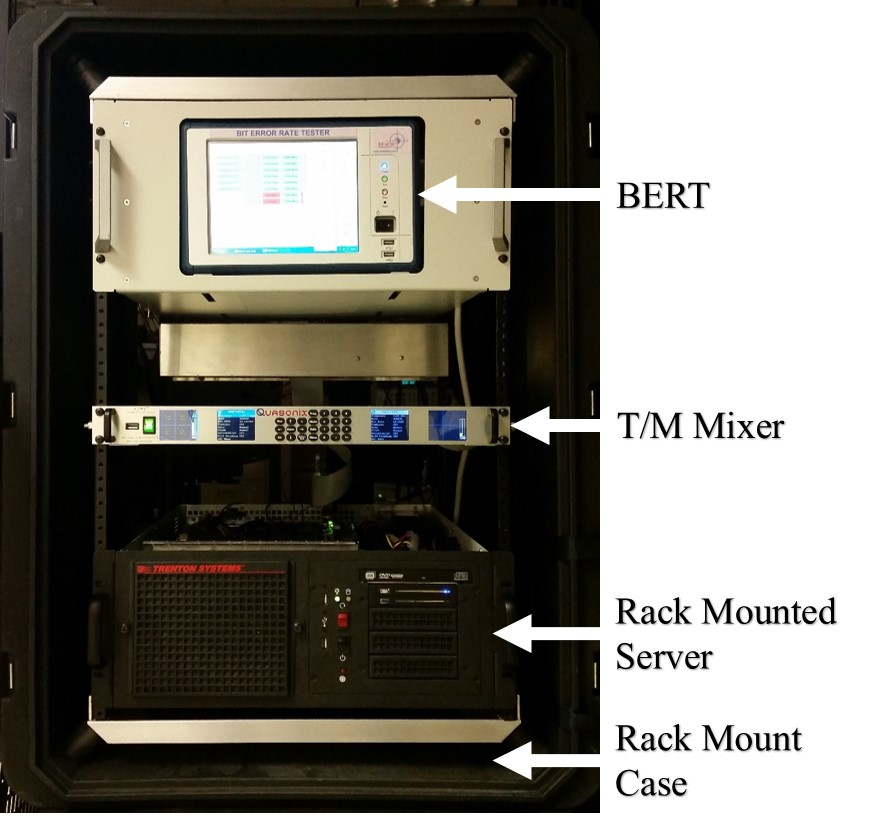
\includegraphics[scale=0.55]{figures/systemOverview/rack.jpg}
%	\caption{A picture of the physical PAQ project hardware. Note that the T/M Receiver is not pictured.}
%	\label{fig:rack}
%\end{figure}
%A picture of the components inside the rack mounted server is shown in Figure \ref{fig:rack}.
%\begin{figure}
%	\centering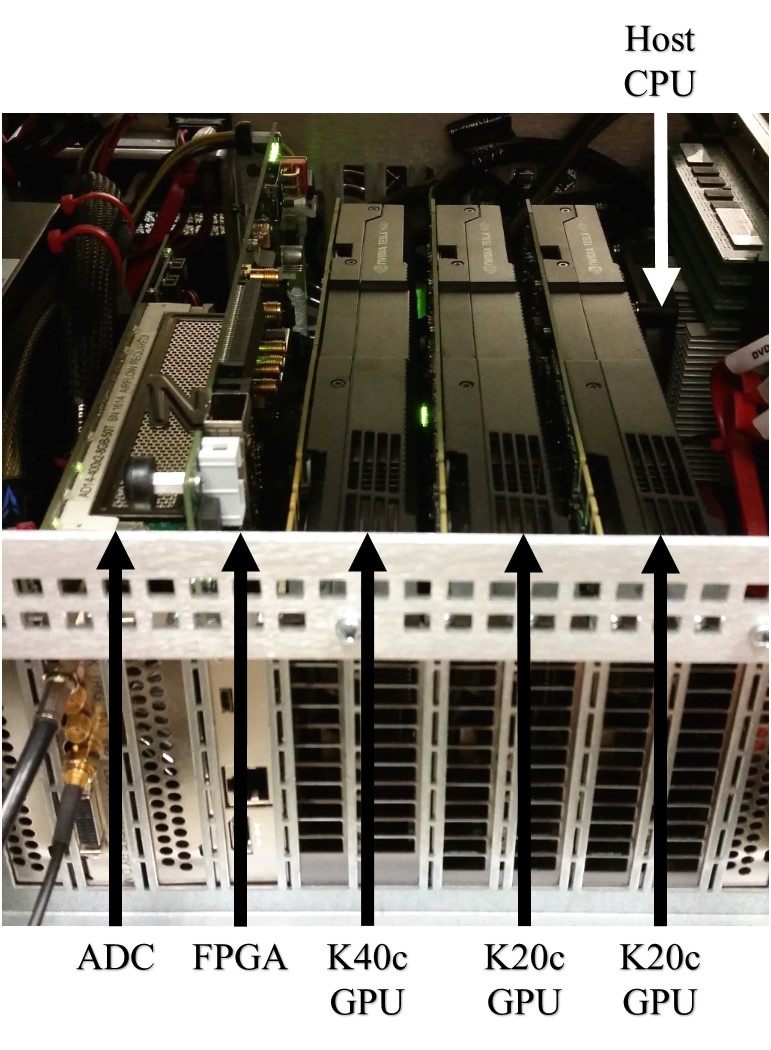
\includegraphics[scale=0.55]{figures/systemOverview/server.jpg}
%	\caption{A pictureof the components inside the rack mounted server.}
%	\label{fig:server}
%\end{figure}

To enable data-aided equalization, the PAQ project bit stream has a packetized structure shown in Figure \ref{fig:packetStructure_intro}.
The bit stream has a pilot bit sequence, in the form of the iNET preamble and ASM, periodically inserted into the data bits.
\begin{figure}
	\centering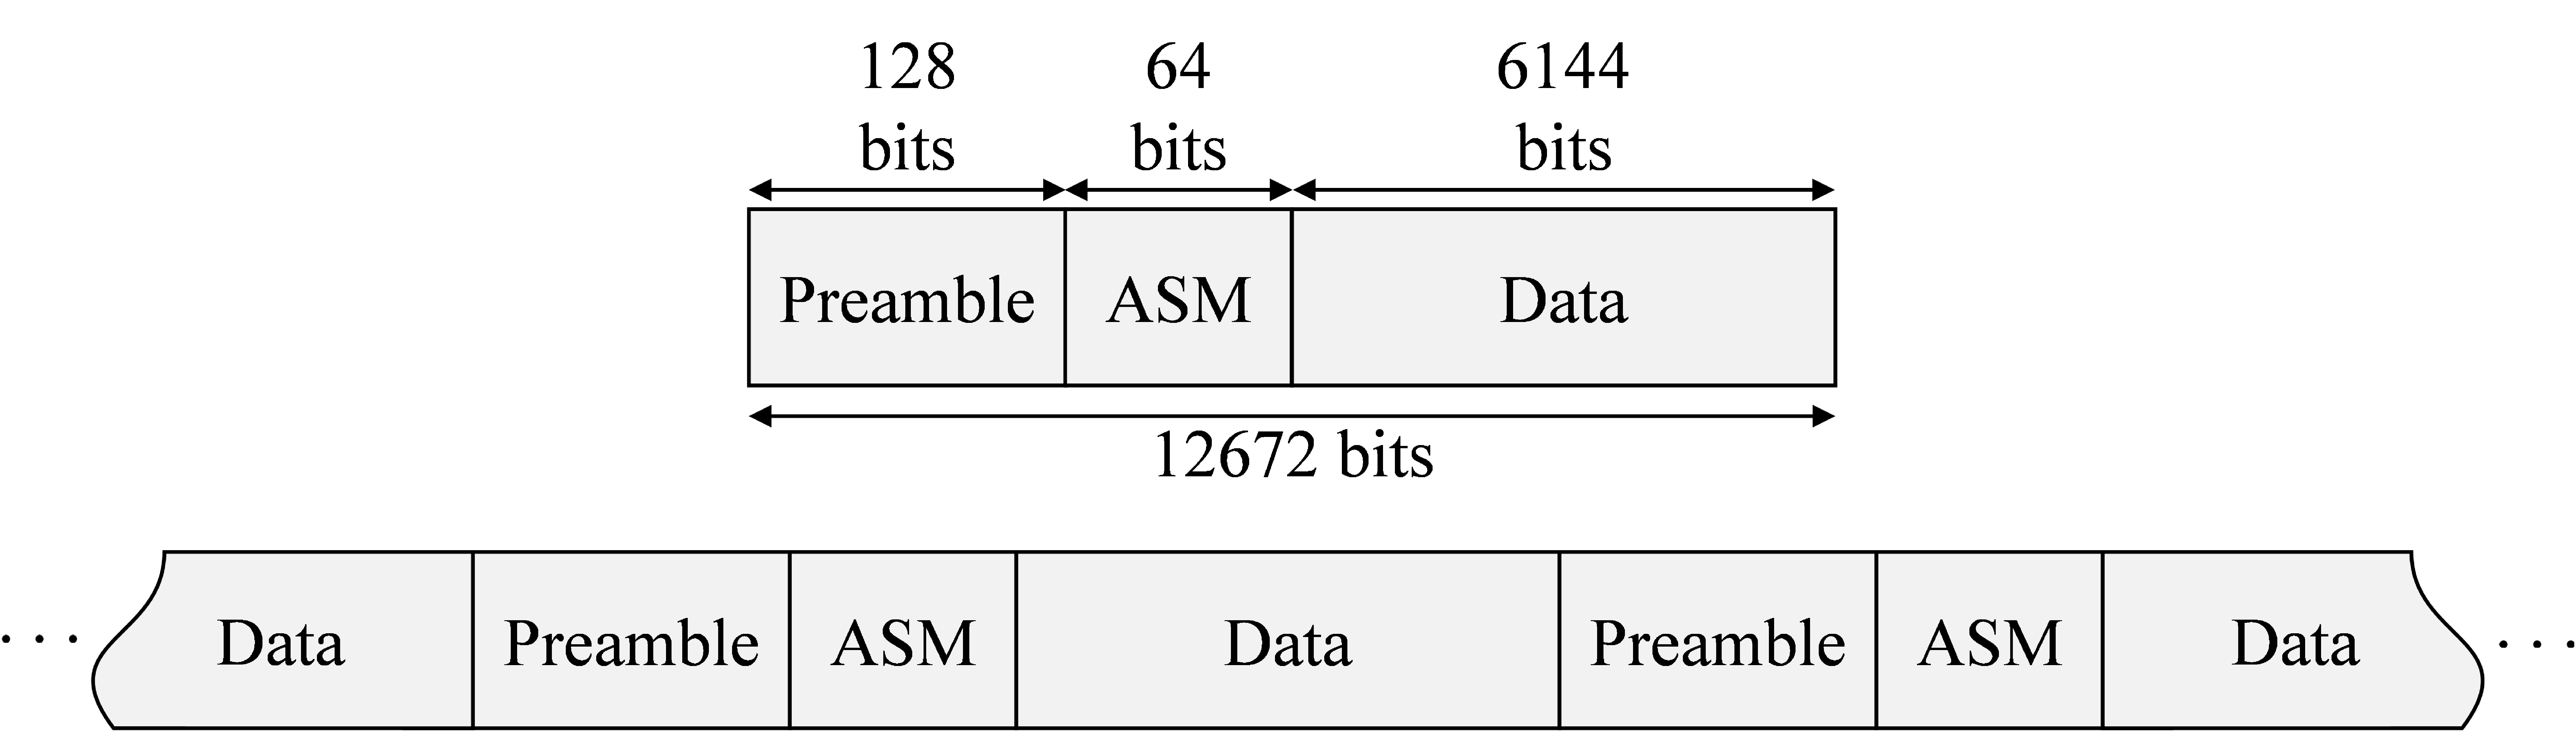
\includegraphics[width=9.47in/100*55]{figures/intro/packetSturcture.pdf}
	\caption{A diagram showing the PAQ packetized sample structure.}
	\label{fig:packetStructure_intro}
\end{figure}
The iNET preamble comprises eight repetitions of the 16-bit sequence $\text{CD98}_\text{hex}$ and the ASM field is
\begin{equation}
\text{034776C7272895B0}_\text{hex}.
\end{equation}
The data payload is a known length-$(2^{11} - 1)$ PN sequence.
Each packet contains $128$ preamble bits, $64$ ASM bits and $6{,}144$ data bits making each iNET packet $6{,}336$ bits.
The data bits modulate a SOQPSK-TG carrier at $10$ Mbits/second.
With the preamble and ASM periodically inserted, the over the air bit rate is $10.3125$ Mbits/second.

After modulation, the transmitted signal experiences multipath interference modeled as the channel $h(t)$.
The transmitted signal also experiences a frequency offset $\omega_0$, a phase offset $\phi$ and additive white Gaussian noise $w(t)$.
The received signal is down-converted, filtered in the T/M mixer, sampled at $93\nicefrac{1}{3}$ Msamples/second by the ADC then down-converted again to baseband and resampled by $\nicefrac{99}{448}$ in the GPUs resulting in the sampled sequence $r(n)$ at rate $20.625$ Msamples/second or $2$ samples/bit.

The model of the received signal is shown in Figure \ref{fig:received1}.
At baseband and $2$ samples/bit, the FIR channel impulse response is assumed to have a non-causal component comprising $N_1$ samples and a causal component comprising $N_2$ samples.
Figure \ref{fig:channelExample} shows the full discrete-time $L_h = N_1+N_2+1$ sample channel.
The received signal is sampled at $20.625$ Msamples/second.
The iNET packet is $\Lpkt=12672$ samples long with the preamble $L_\text{p}=256$ samples and the ASM $L_\text{ASM}=128$ samples.
\begin{figure}
	\centering
\includegraphics[width=12.33in/100*50]{figures/intro/received1.pdf}
	\caption{Received signal has multipath interference, frequency offset, phase offset and additive white Gaussian noise. The received signal is down-converted filtered and sampled to produce the sample sequence $r(n)$.}
	\label{fig:received1}
\end{figure}
\begin{figure}
	\centering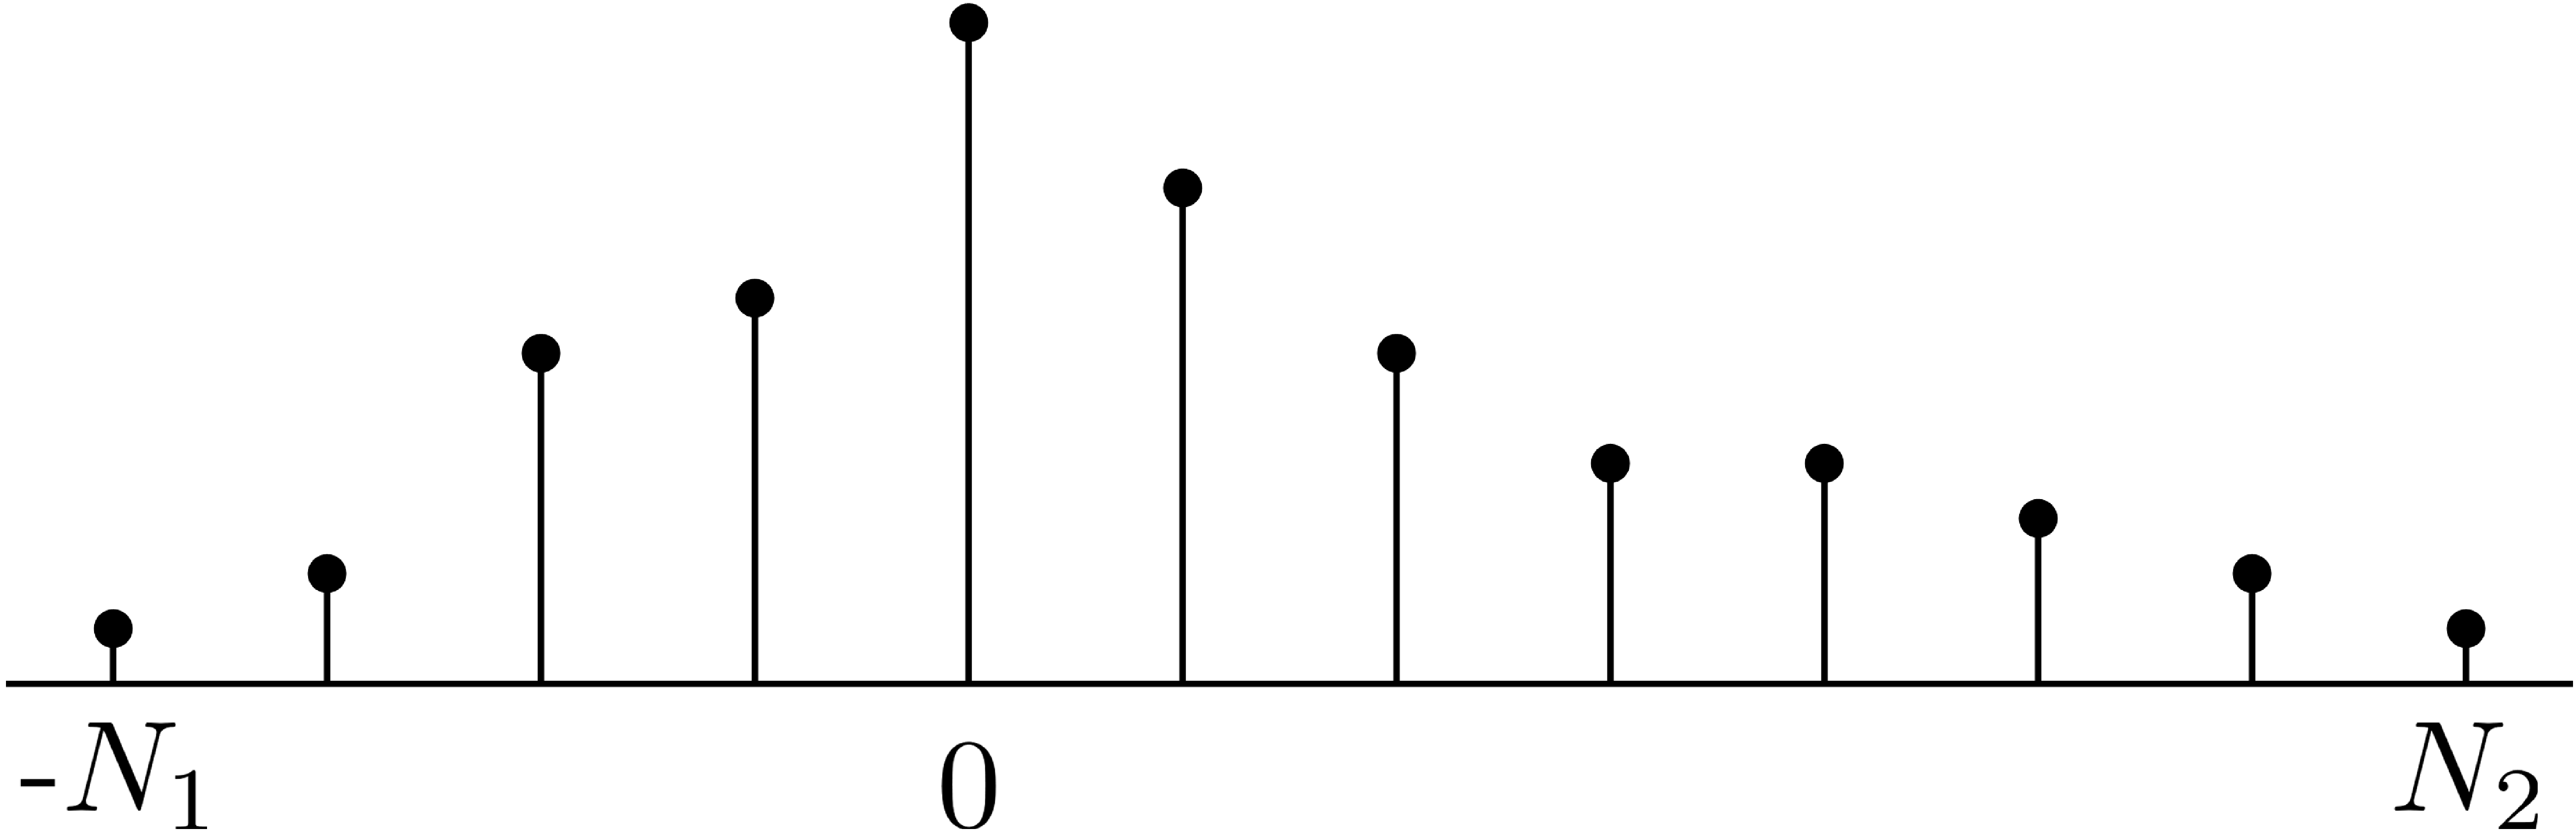
\includegraphics[width=5.5in/100*55]{figures/intro/channelExample.pdf}
	\caption{An illustration of the discrete-time channel of length $N_1+N_2+1$ with a non-causal component comprising $N_1$ samples and a causal component comprising $N_2$ samples.}
	\label{fig:channelExample}
\end{figure}

\section{Digital Signal Processing}
\label{sec:signalProcessing}
A high-level digital signal processing flow is shown in Figure \ref{fig:estimators} and \ref{fig:thisThesisBlock}.
Because the frequency offset, channel, and noise variance are estimated using the preamble and ASM, the first step is to find the samples correlating to the preamble in the received sample sequence $r(n)$.
The preamble detector block correlates received samples with $L_\text{P}$ samples of a locally stored copy of the pilot in \eqref{eq:preamble_ASM}.
The preamble detector block outputs the vector of samples $\mathbf{r}_\text{p}$ with the iNET packetized structure.
The first $L_\text{P} + L_\text{ASM}$ samples in $\mathbf{r}_\text{p}$ correlate with the received pilot samples.
\begin{equation}
\mathbf{p} = \big[ p(0) \quad p(1) \quad \cdots  \quad  p(L_\text{P} + L_\text{ASM}-1) \big]
\label{eq:preamble_ASM}
\end{equation}

The located preamble samples are used first to estimate the frequency offset.
The estimated frequency offset $\hat{\omega}_0$ rads/sample is then used to ``de-rotate'' the vector of samples $\mathbf{r}_\text{p}$ to produce $\mathbf{r}$.
The de-rotated samples in the vector $\mathbf{r}$ that correlate to the preamble and ASM are used to estimate the channel $\hat{\mathbf{h}}$ and noise variance $\hat{\sigma}^2_w$.
The channel and noise variance estimates are done in the estimators block.
\begin{figure}
	\centering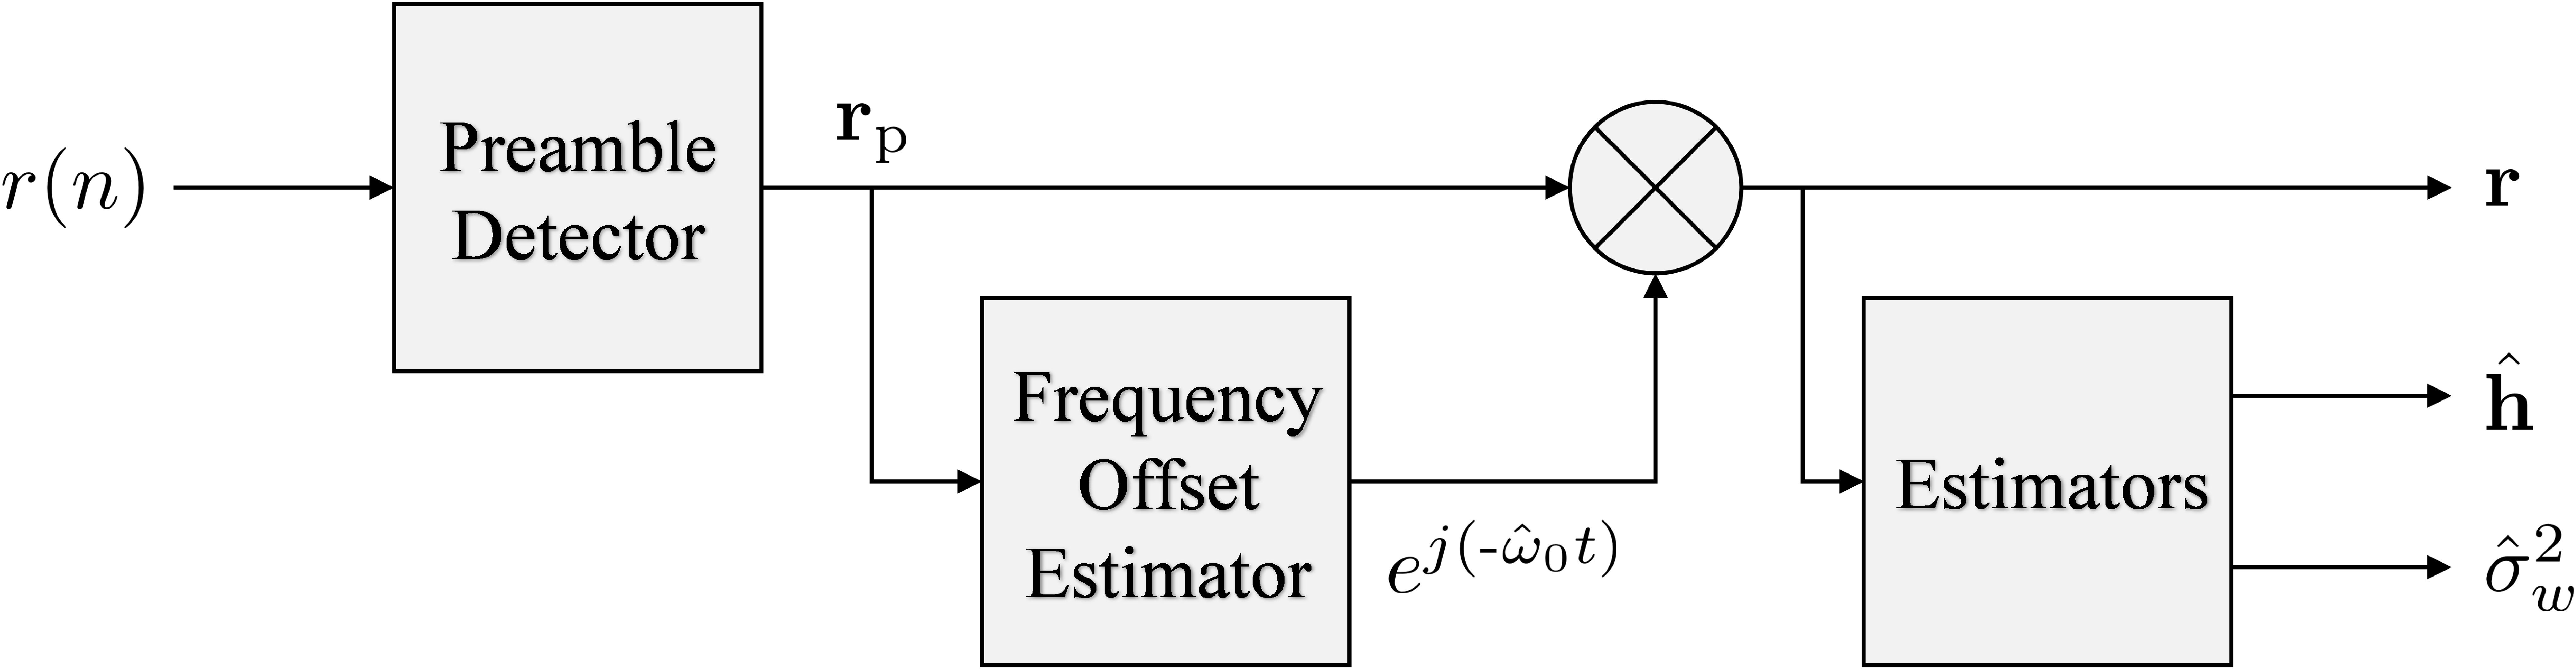
\includegraphics[width=8.75in/100*55]{figures/intro/estimators.pdf}
	\caption{A block diagram of the estimators in the PAQ project.}
	\label{fig:estimators}
\end{figure}

Equipped with knowledge of the estimated channel and noise variance, data-aided finite impulse response (FIR) equalizer filters can be computed.
The all the data-aided equalizer filters are computed using the same channel and noise variance estimates.
The blocks shown in Figure \ref{fig:thisThesisBlock} are duplicated in five independent branches producing five estimated vectors of bits $\hat{\mathbf{b}}$, one for each equalizer.

%An equalizer filter is computed using the channel estimate $\hat{\mathbf{h}}$ and noise variance $\hat{\sigma}^2_w$ then applied to the vector of samples $\mathbf{r}$.
The PAQ project designed the data-aided FIR equalizer filters to be $5$ times longer than the channel estimate. The equalizer filter has a non-causal component comprising $L_1 = 5N_1 = 60$ samples and a causal component comprising $L_2 = 5N_2 = 125$ samples.
The $L_\text{EQ} = L_1+L_2+1$ sample full discrete-time equalizer filters are computed and applied in the equalizer filter block.

The output of the equalizer filters are then filtered by a SOQPSK-TG detection filter and down-sampled by $2$ in preparation for an OQPSK detector.
The $\mathbf{r}_\text{d}$ in each equalizer branch has a sample rate of $1$ sample/bit or $2$ samples/symbol.
The OQPSK detector block outputs the vector of estimated bits $\hat{\mathbf{b}}$.
\begin{figure}
	\centering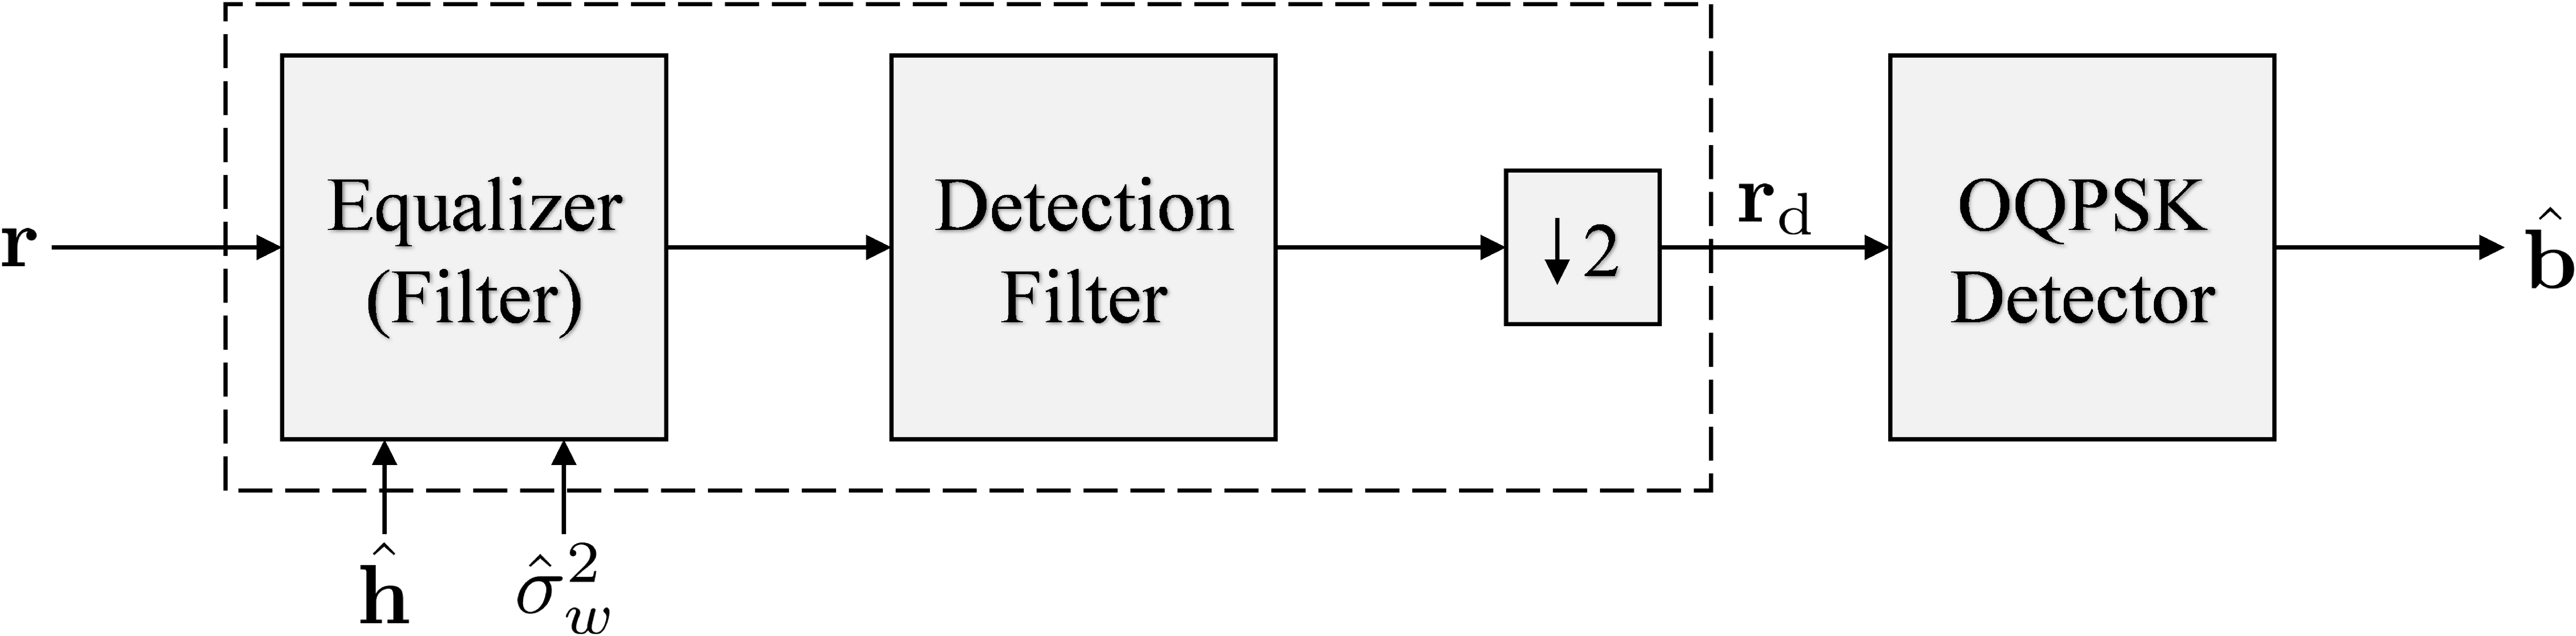
\includegraphics[width=8.37in/100*55]{figures/intro/thisThesisBlock.pdf}
	\caption{A block diagram of application of the FIR equalizer and detection filters in the Preamble Assisted Equalization (PAQ) project.}
	\label{fig:thisThesisBlock}
\end{figure}
Finally the BER for each equalizer is obtained by comparing the vectors of estimated bits $\hat{\mathbf{b}}$ to the PN sequence.

The GPUs in Figure \ref{fig:hardwareblock} and \ref{fig:HostSystem} perform all the digital signal processing in parallel.
To introduce as much parallelism as possible, the received samples are processed in $39$,$321$,$600$ sample 		sets. 
At $20.625$ Msamples/second, each set of $39$,$321$,$600$ samples is $1907$ milliseconds worth of data.
Each set has at most $3104$ independent $12672$ sample iNET packets.
The GPU processes $3104$ packets in parallel by leveraging batched processing.
Each packet is a batch and each batch performs the algorithms shown in Figures \ref{fig:estimators} and \ref{fig:thisThesisBlock}.
In order to stay real-time, \textbf{all} processing must be completed in $1907$ ms.

This thesis, will illustrate how the five PAQ data-aided equalizers were computed and applied to the received samples in GPUs.
The dashed box in Figure \ref{fig:thisThesisBlock} emphasizes which processing blocks are focused on.

Chapter \ref{chap:equations} shows the equations for these block diagrams.
Chapter \ref{chap:gpu} will shed some light on signal processing in GPUs.
Chapter \ref{chap:equalizers_in_gpus} will illustrate how the five equalizers are implemented in GPUs.
Chapter \ref{chap:final_summary} will summarize.
\chapter{Signal Processing in GPUs}
\label{chap:gpu}
A Graphics Processing Unit (GPU) is a computational unit with a highly-parallel architecture well-suited for executing the same function on many data elements.
In the past, GPUs were used to process graphics data but in 2008 NVIDIA released the Tesla GPU.
Telsa GPUs are built for general purpose high performance computing.
Figure \ref{fig:GPUpicture} shows the form factor of a Tesla K40c and K20c.
\begin{figure}
	\centering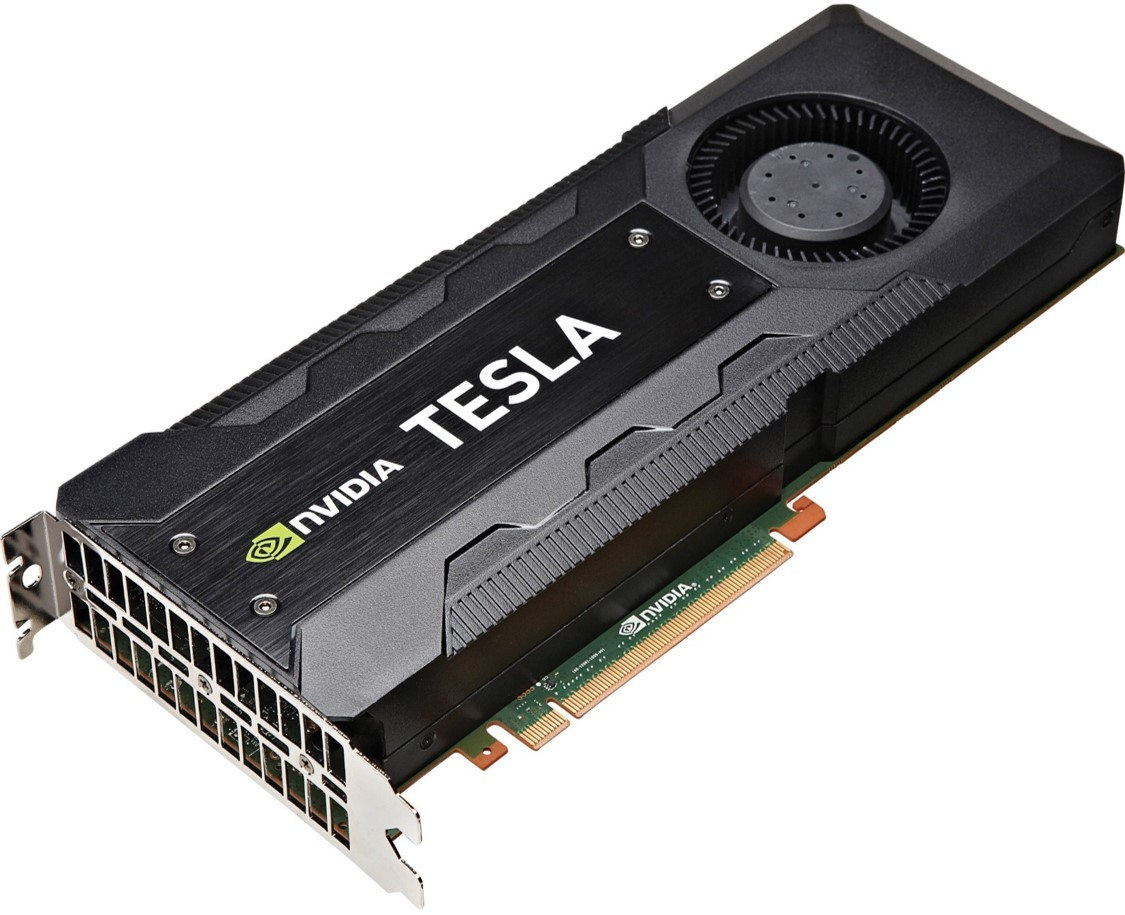
\includegraphics[width=5in]{figures/gpu_intro/k40c_k20c.jpg}
	\caption{NVIDIA Tesla K40c and K20c.}
	\label{fig:GPUpicture}
\end{figure}

In 2007 NVIDIA released an extension to C, C++ and Fortran called CUDA (Compute Unified Device Architecture).
CUDA enables GPUs to be used for high performance computing in computer vision, deep learning, artificial intelligence and signal processing \cite{wikipedia-gpu:2015}.
CUDA allows a programmer to write C++ like functions that are massively parallel called \textit{kernels}.
To invoke parallelism, a GPU kernel executed $N$ times with the work distributed to $N_\text{min}$ total \textit{threads} that run concurrently.
To achieve the full potential of high performance GPUs, kernels must be written with some basic concepts about GPU architecture and memory in mind.
This chapter will show the following:
\begin{itemize}
\item Optimizing memory access leads to faster execution time rather than optimizing number of floating point operations.
\item The number of threads per block can significantly affect execution time.
\item CPU and GPU processing can be pipelined.
\item Convolution maps very well to GPUs using the Fast Fourier Transform (FFT).
\item Batched processing leads to faster execution time per batch.
\end{itemize}

\section{GPU and CUDA Introduction}
\subsection{An Example Comparing CPU and GPU}
If a programmer has some C++ experience, learning how to program GPUs using CUDA comes fairly easily.
GPU code still runs top to bottom and memory still has to be allocated.
The only real difference is the physical location of the memory and how functions run on GPUs.
To run functions or kernels on GPUs, the memory must be copied from the host (CPU) to the device (GPU).
Once the memory has been copied, parallel GPU kernels operate on the data.
After GPU kernel execution, results are usually copied back from the device (GPU) to the host (CPU).

Listing \ref{code:GPUvsCPU} shows a simple program that implements real-valued float vector addition in a CPU and a GPU.
The vector $\mathbf{C}_1$ is the sum of the vectors $\mathbf{A}_1$ and $\mathbf{B}_1$ computed in the CPU.
The vector $\mathbf{C}_2$ is the sum of the vectors $\mathbf{A}_2$ and $\mathbf{B}_2$ computed in the GPU.
Line $42$ the CPU computes $\mathbf{C}_1$ by summing elements of $\mathbf{A}_1$ and $\mathbf{B}_1$ together \textit{sequentially}. Figure \ref{fig:CPUaddBlockDiagram} shows how the CPU 
sequentially computes one element of $\mathbf{C}_1$ at time by summing one element from $\mathbf{A}_1$ and one element $\mathbf{B}_1$.

The GPU performs all the summations in parallel because each element of $\mathbf{C}_2$ is independent of all other elements. 
Before the computation of $\mathbf{C}_2$ can execute on the GPU, the vectors in host memory $\mathbf{A}_1$ and $\mathbf{B}_1$ are copied to device memory vectors $\mathbf{A}_2$ and $\mathbf{B}_2$ as shown on lines $60$ and $61$.
Once $\mathbf{A}_2$ and $\mathbf{B}_2$ are on the GPU, the vector $\mathbf{C}_2$ is computed by calling the GPU kernel VecAddGPU on line $75$.
VecAddGPU computes all the elements of $\mathbf{C}_2$ by performing a summation of all the elements of $\mathbf{A}_2$ and $\mathbf{B}_2$.
The vector $\mathbf{C}_2$ is then copied from device memory to host memory on line $78$.
Figure \ref{fig:GPUaddBlockDiagram} shows how the GPU computes $\mathbf{C}_2$ \textit{in parallel}.

\begin{figure}
	\centering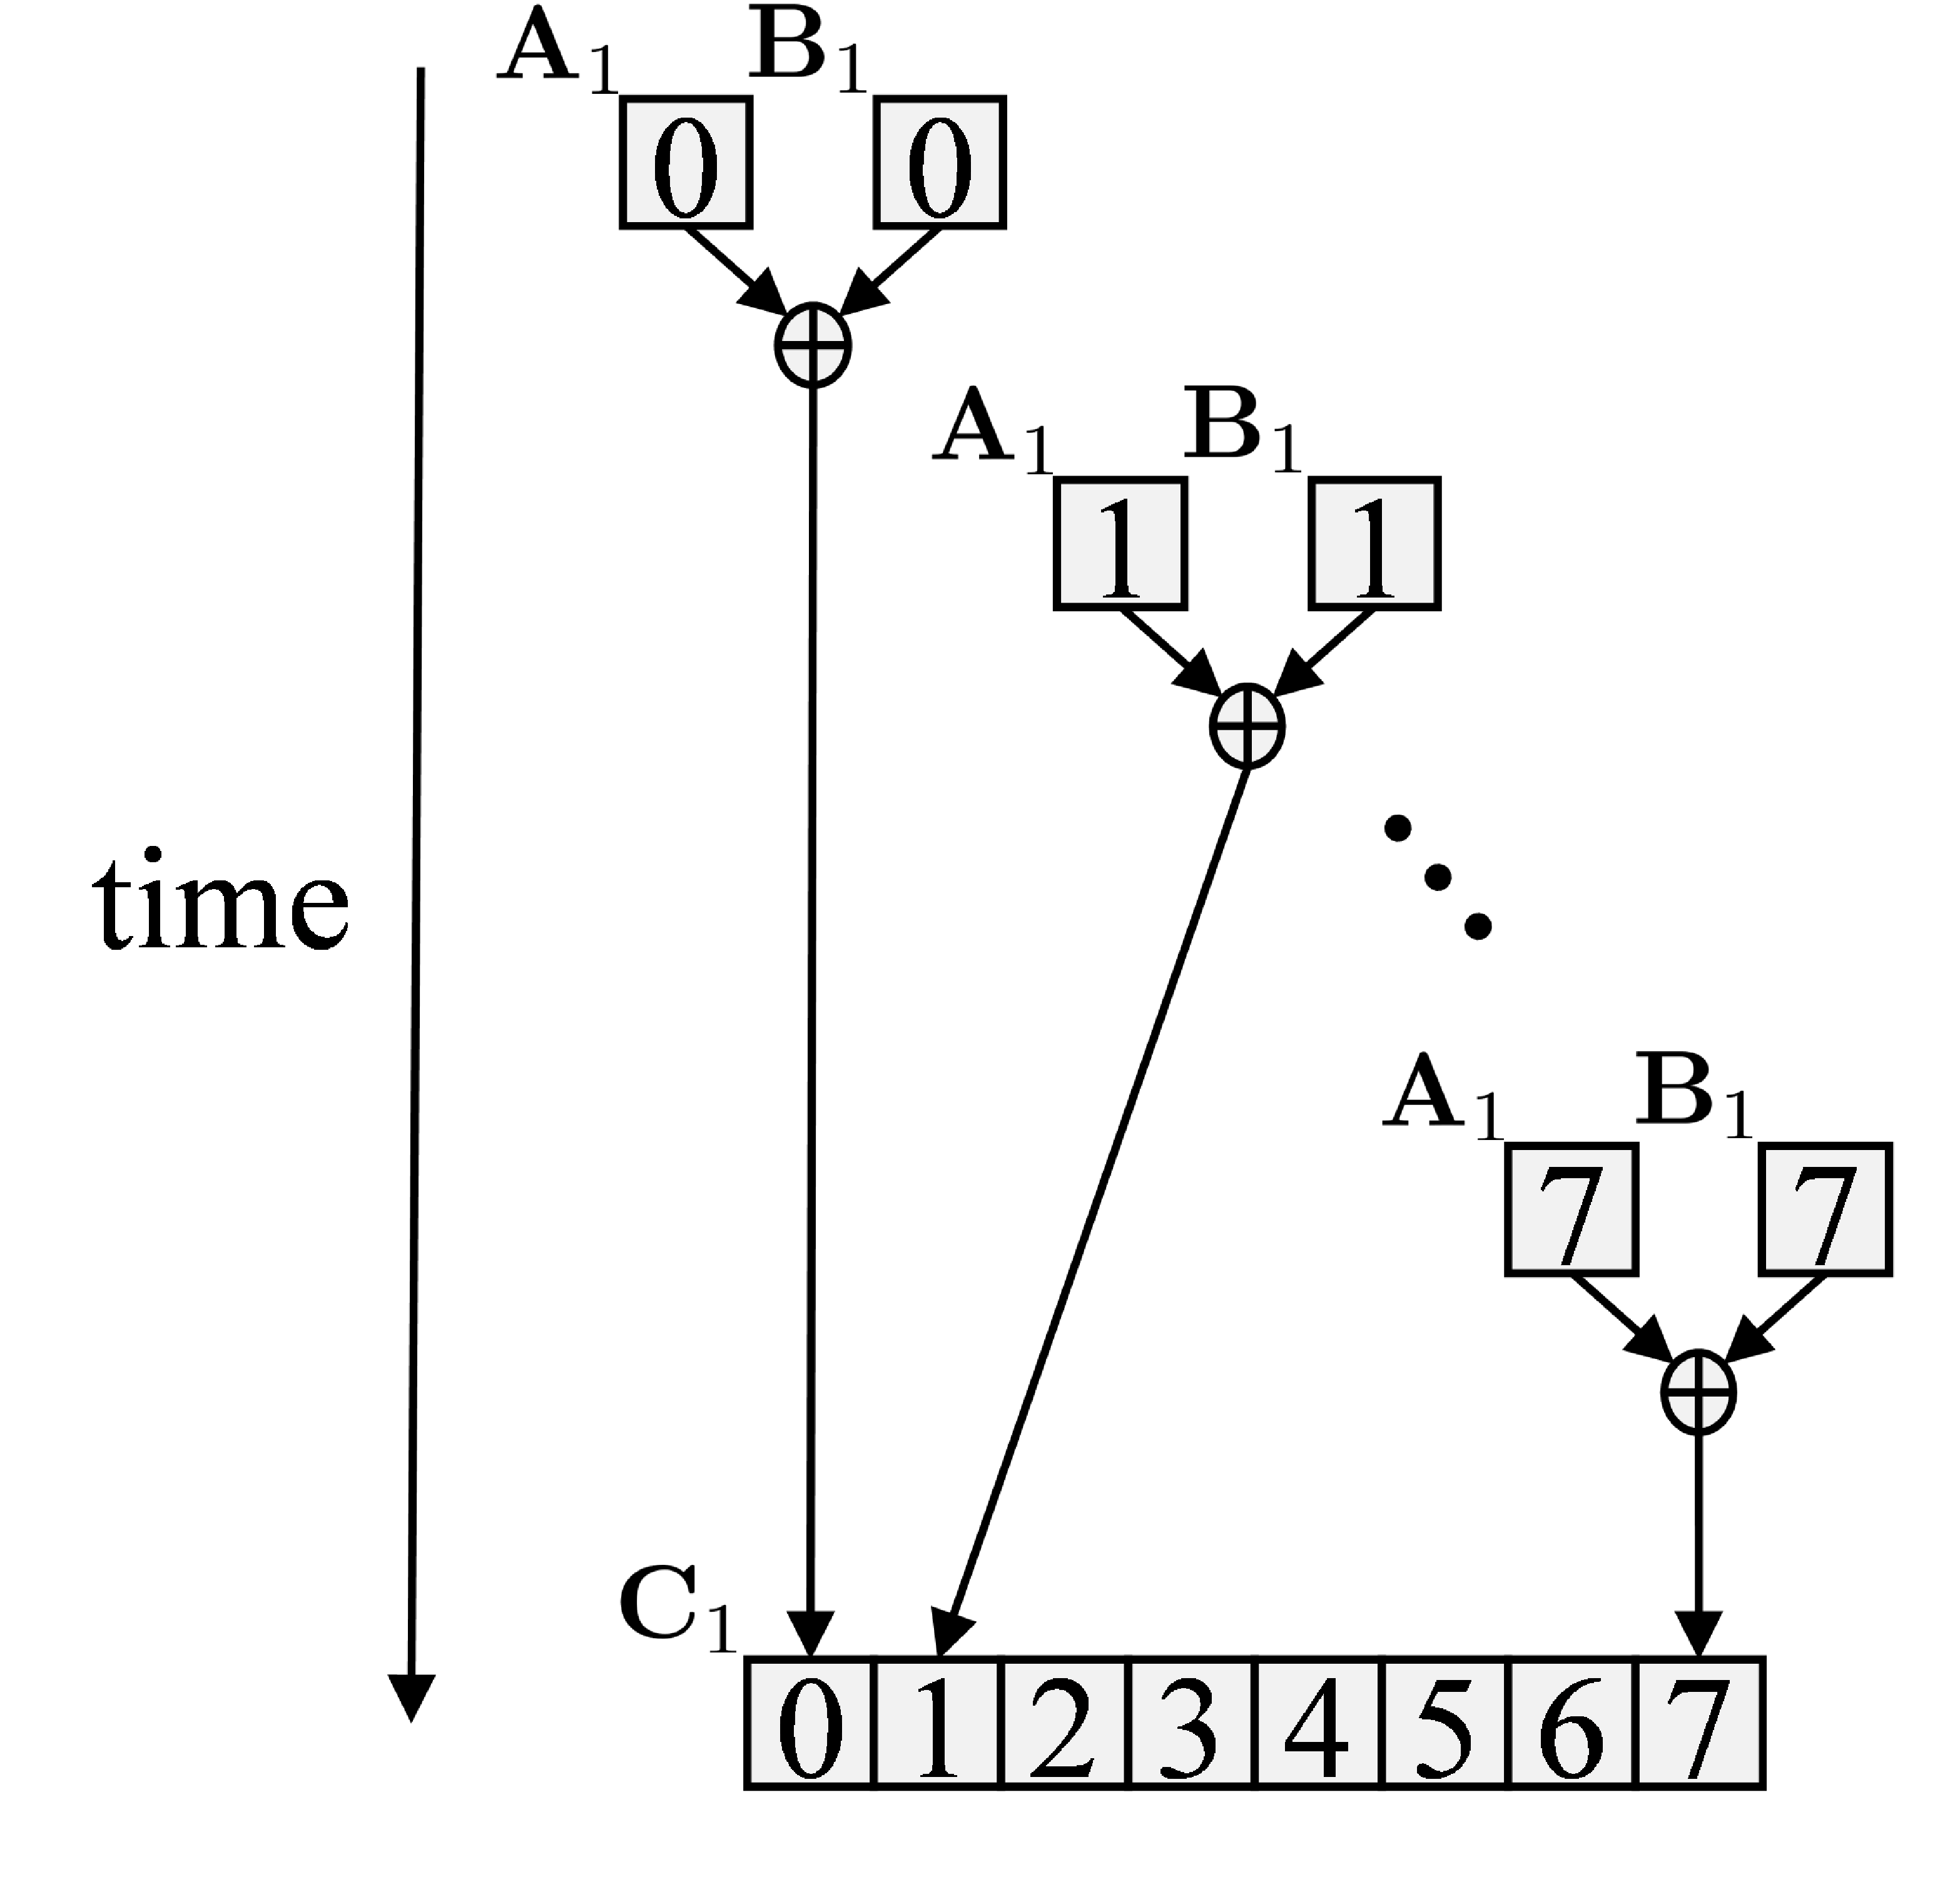
\includegraphics[width=3.17in/100*55]{figures/gpu_intro/CPUaddBlockDiagram.pdf}
	\caption{A block diagram of how a CPU sequentially performs vector addition.}
	\label{fig:CPUaddBlockDiagram}
\end{figure}
\begin{figure}
	\centering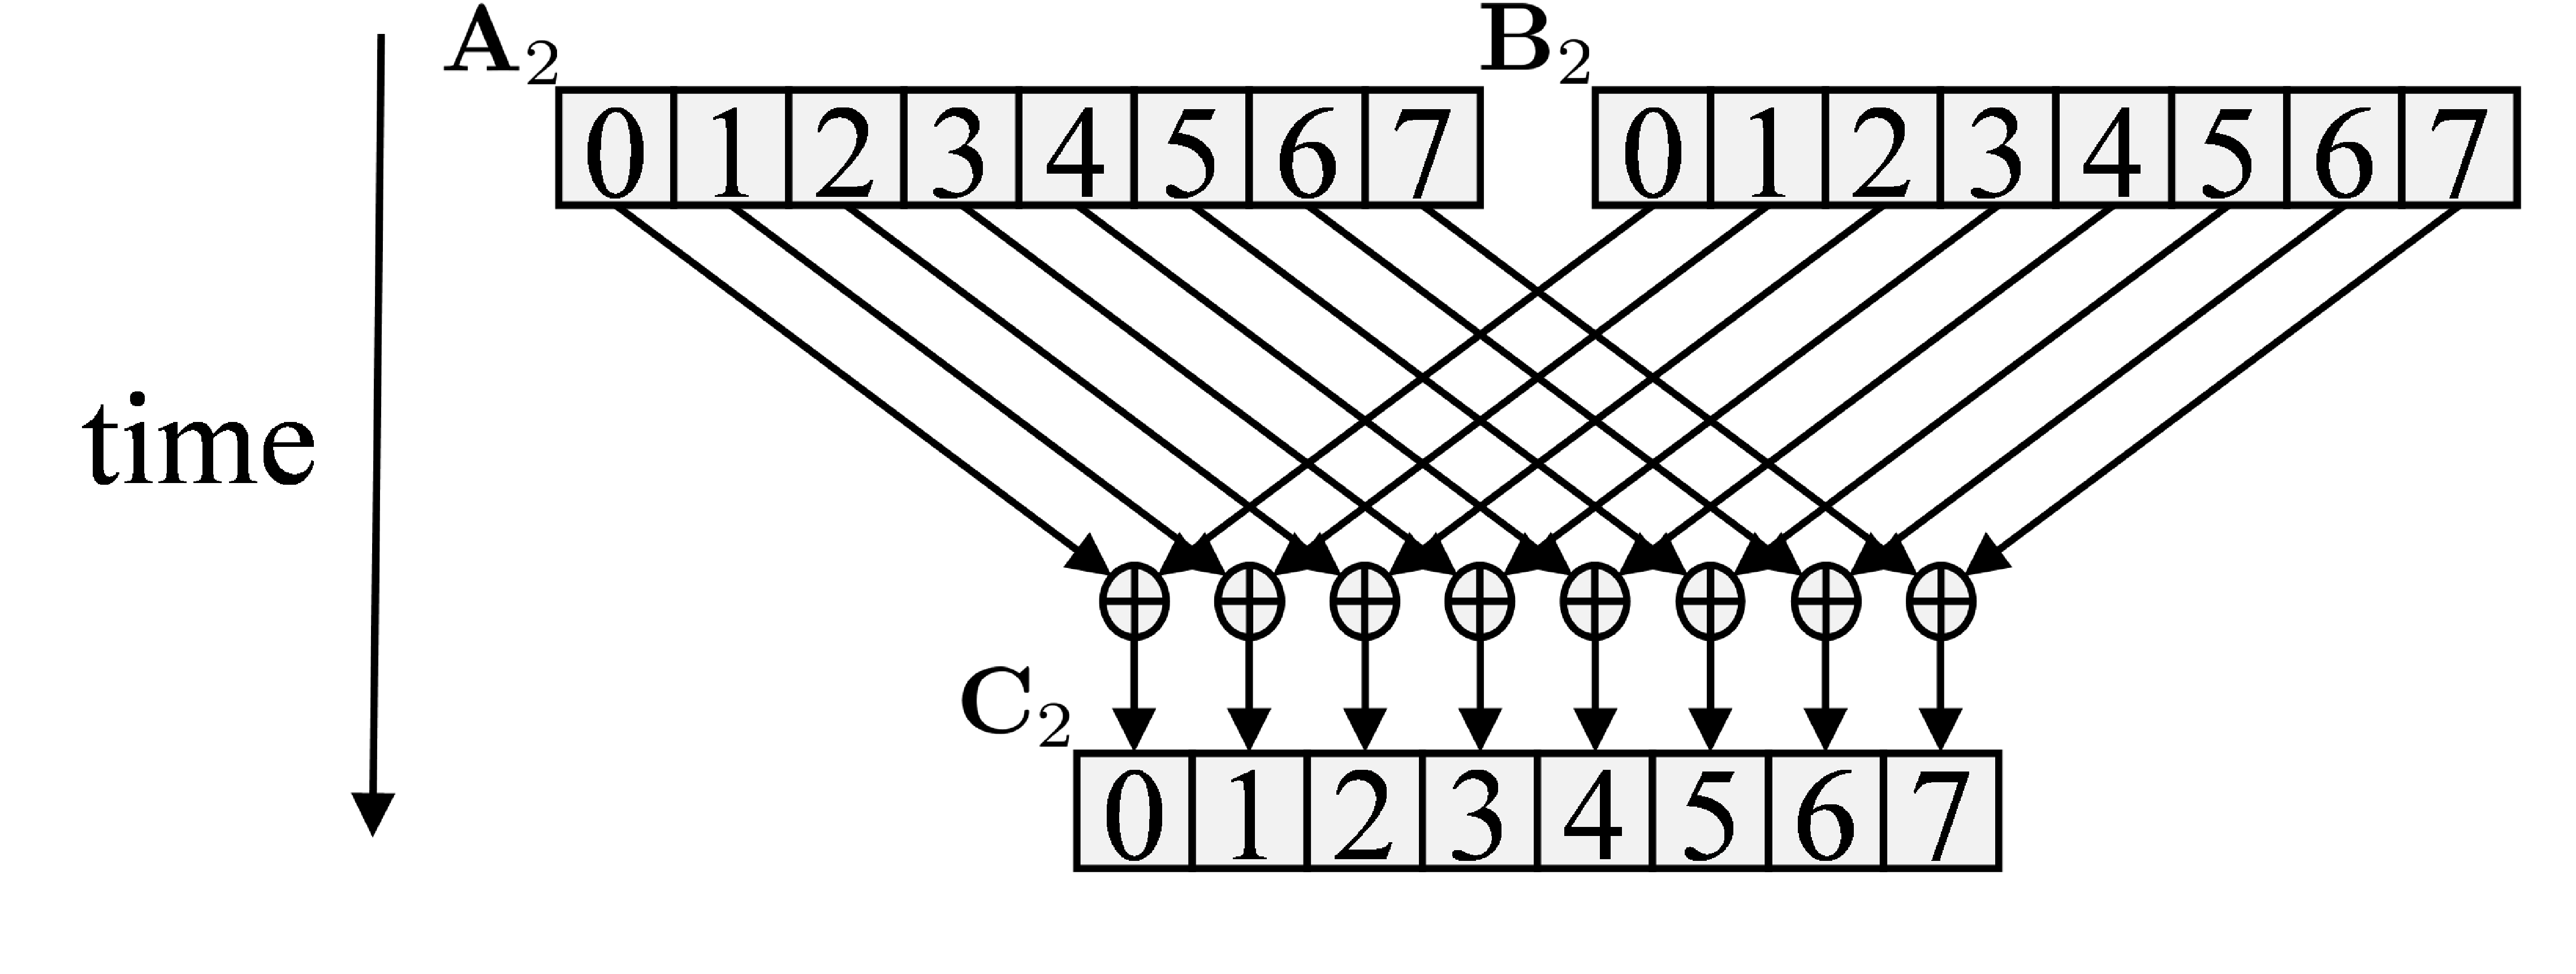
\includegraphics[width=4.69in/100*55]{figures/gpu_intro/GPUaddBlockDiagram.pdf}
	\caption{A block diagram of how a GPU performs vector addition in parallel.}
	\label{fig:GPUaddBlockDiagram}
\end{figure}

\singlespacing
\clearpage
\begin{lstlisting}[style=myCUDAstyle,caption={Comparison of CPU and GPU code.},label={code:GPUvsCPU}]
#include <iostream>
#include <stdlib.h>
#include <math.h>
using namespace std;

void VecAddCPU(float* destination,float* source0,float* source1,int myLength){
	for(int i = 0; i < myLength; i++)
		destination[i] = source0[i] + source1[i];
}

__global__ void VecAddGPU(float* destination, float* source0, float* source1, int lastThread){
	int i = blockIdx.x*blockDim.x + threadIdx.x;

	// don't access elements out of bounds
	if(i >= lastThread)
		return;

	destination[i] = source0[i] + source1[i];
}

int main(){
	int N = pow(2,22);
	cout << N << endl;
	/**
	* Vector Addition on CPU
	*/
	// allocate memory on host
	float *A1;
	float *B1;
	float *C1;
	A1 = (float*) malloc (N*sizeof(float));
	B1 = (float*) malloc (N*sizeof(float));
	C1 = (float*) malloc (N*sizeof(float));

	// Initialize vectors 0-99
	for(int i = 0; i < N; i++){
		A1[i] = rand()%100;
		B1[i] = rand()%100;
	}

	// vector sum C1 = A1 + B1
	VecAddCPU(C1, A1, B1, N);
	
	/**
	* Vector Addition on GPU
	*/
	// allocate memory on host for result
	float *C2;
	C2 = (float*) malloc (N*sizeof(float));

	// allocate memory on device for computation
	float *A2_gpu;
	float *B2_gpu;
	float *C2_gpu;
	cudaMalloc(&A2_gpu, sizeof(float)*N);
	cudaMalloc(&B2_gpu, sizeof(float)*N);
	cudaMalloc(&C2_gpu, sizeof(float)*N);

	// Copy vectors A and B from host to device
	cudaMemcpy(A2_gpu, A1, sizeof(float)*N, cudaMemcpyHostToDevice);
	cudaMemcpy(B2_gpu, B1, sizeof(float)*N, cudaMemcpyHostToDevice);

	// Set optimal number of threads per block
	int T_B = 32;

	// Compute number of blocks for set number of threads
	int B = N/T_B;

	// If there are left over points, run an extra block
	if(N % T_B > 0)
		B++;

	// Run computation on device
	//for(int i = 0; i < 100; i++)
	VecAddGPU<<<B, T_B>>>(C2_gpu, A2_gpu, B2_gpu, N);

	// Copy vector C2 from device to host
	cudaMemcpy(C2, C2_gpu, sizeof(float)*N, cudaMemcpyDeviceToHost);

	// Compare C2 to C1
	bool equal = true;
	for(int i = 0; i < N; i++)
		if(C1[i] != C2[i])
			equal = false;
	if(equal)
		cout << "C2 is equal to C1." << endl;
	else
		cout << "C2 is NOT equal to C1." << endl;

	// Free vectors on CPU
	free(A1);
	free(B1);
	free(C1);
	free(C2);

	// Free vectors on GPU
	cudaFree(A2_gpu);
	cudaFree(B2_gpu);
	cudaFree(C2_gpu);
}
\end{lstlisting}
\doublespacing

\subsection{GPU kernel using threads and thread blocks}
A GPU kernel is executed by launching blocks with a set number of threads per block.
In the Listing \ref{code:GPUvsCPU}, VecAddGPU is launched on line 75 with $32$ threads per block.
The total number of threads launched on the GPU is the number of blocks times the number of threads per block.
VecAddGPU needs to be launched with at least $N = 2^{22}$ (line 22) threads or $2^{22}/32$ blocks of $32$ threads.

CUDA gives each thread launched in a GPU kernel a set of unique indices called threadIdx and blockIdx.
threadIdx is the thread index inside the assigned thread block.
blockIdx is the index of the block to which the thread is assigned.
Both threadIdx and blockIdx are three dimensional (i.e. they both have x, y, and z components).
In this thesis only the x dimension is used because the GPU kernels operate only on one dimensional vectors.
blockDim is the number of threads assigned per block, in fact blockDim is equal to the number of threads per block because the vectors are one dimensional.

To convert the CPU ``for loop'' on line 7 to a GPU kernel, at least $N$ threads are launched with $T$ threads per thread block.
The number of blocks needed is $B = \frac{N}{T_B}$ or $B = \frac{N}{T}+1$ if $N$ is not an integer multiple of $T$.
Figure \ref{fig:threadsBlocks32} shows $N = 32$ threads launched in $B = 4$ thread blocks with $T = 8$ threads per block.
Figure \ref{fig:threadsBlocks36} shows $N = 36$ threads launched in $B = 5$ thread blocks with $T = 8$ threads per block. 
An full extra thread block is launched with $T = 8$ threads but $4$ threads are idle.
Note that thread blocks are executed independent of other thread blocks.
The GPU does not guarantee Block $0$ will execute before Block $2$.
\begin{figure}
	\centering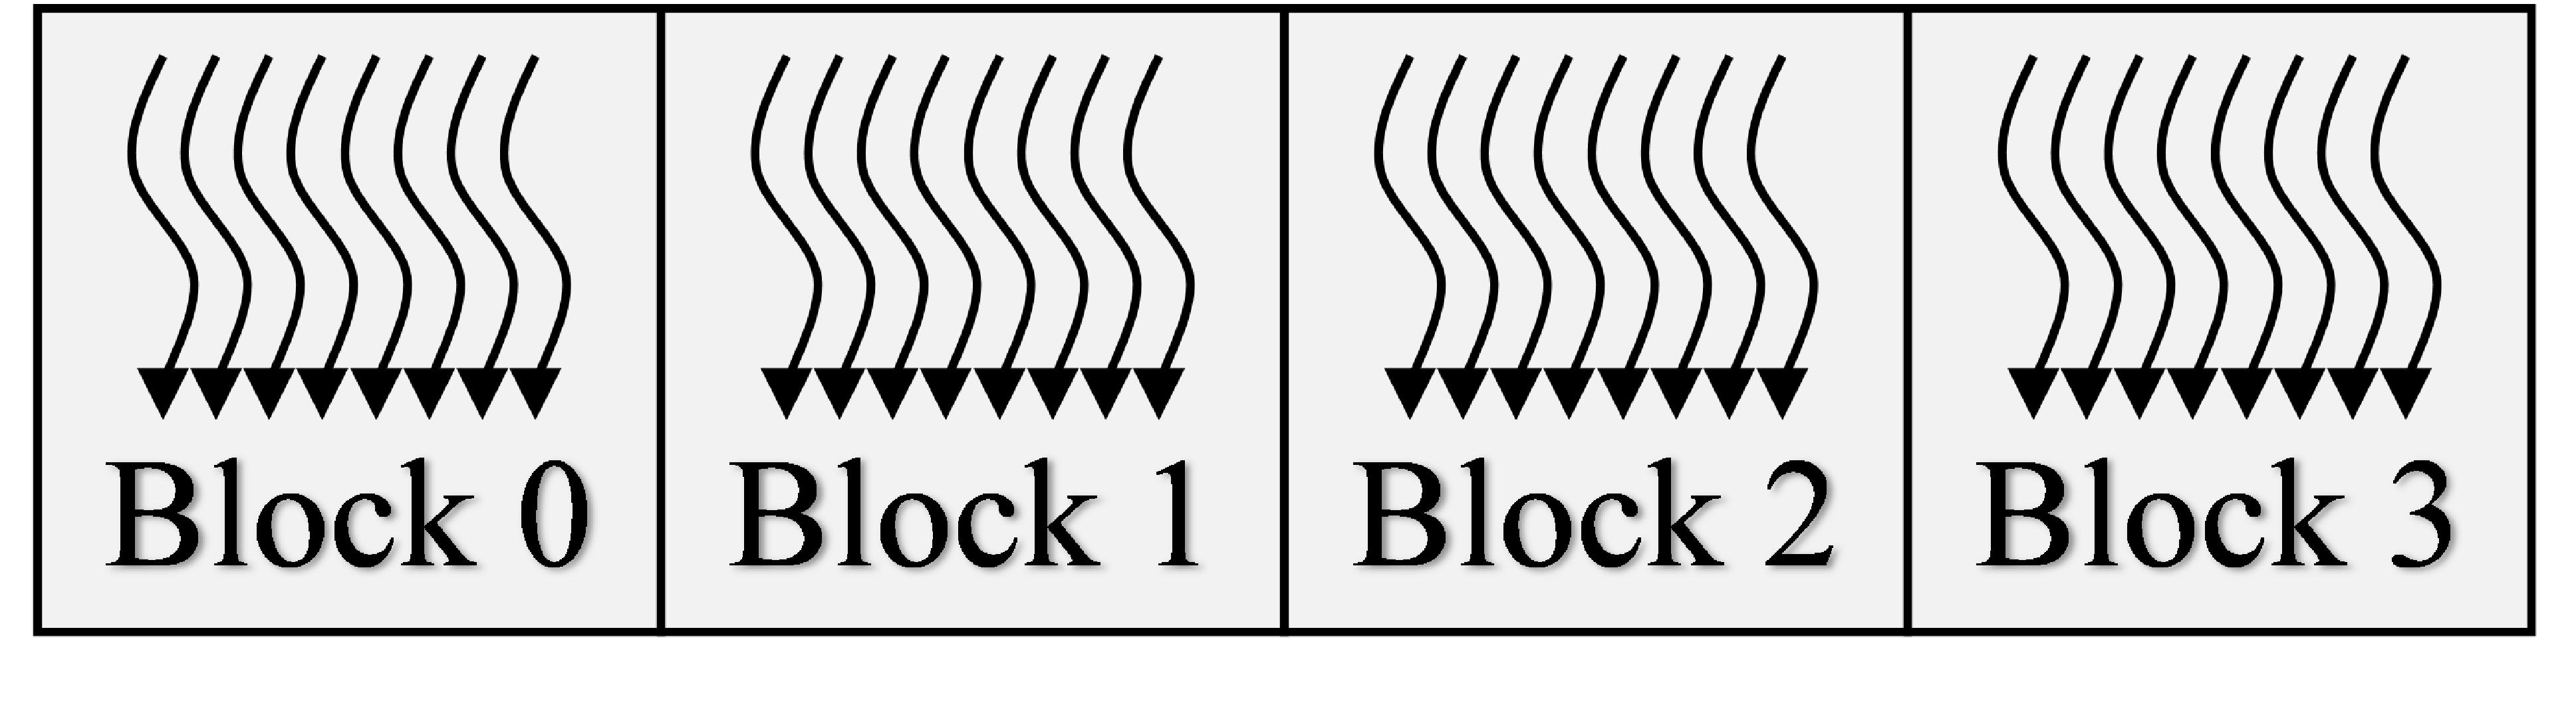
\includegraphics[width=4in/100*55]{figures/gpu_intro/threadsBlocks32.pdf}
	\caption{$32$ threads launched in $4$ thread blocks with $8$ threads per block.}
	\label{fig:threadsBlocks32}
\end{figure}
\begin{figure}
	\centering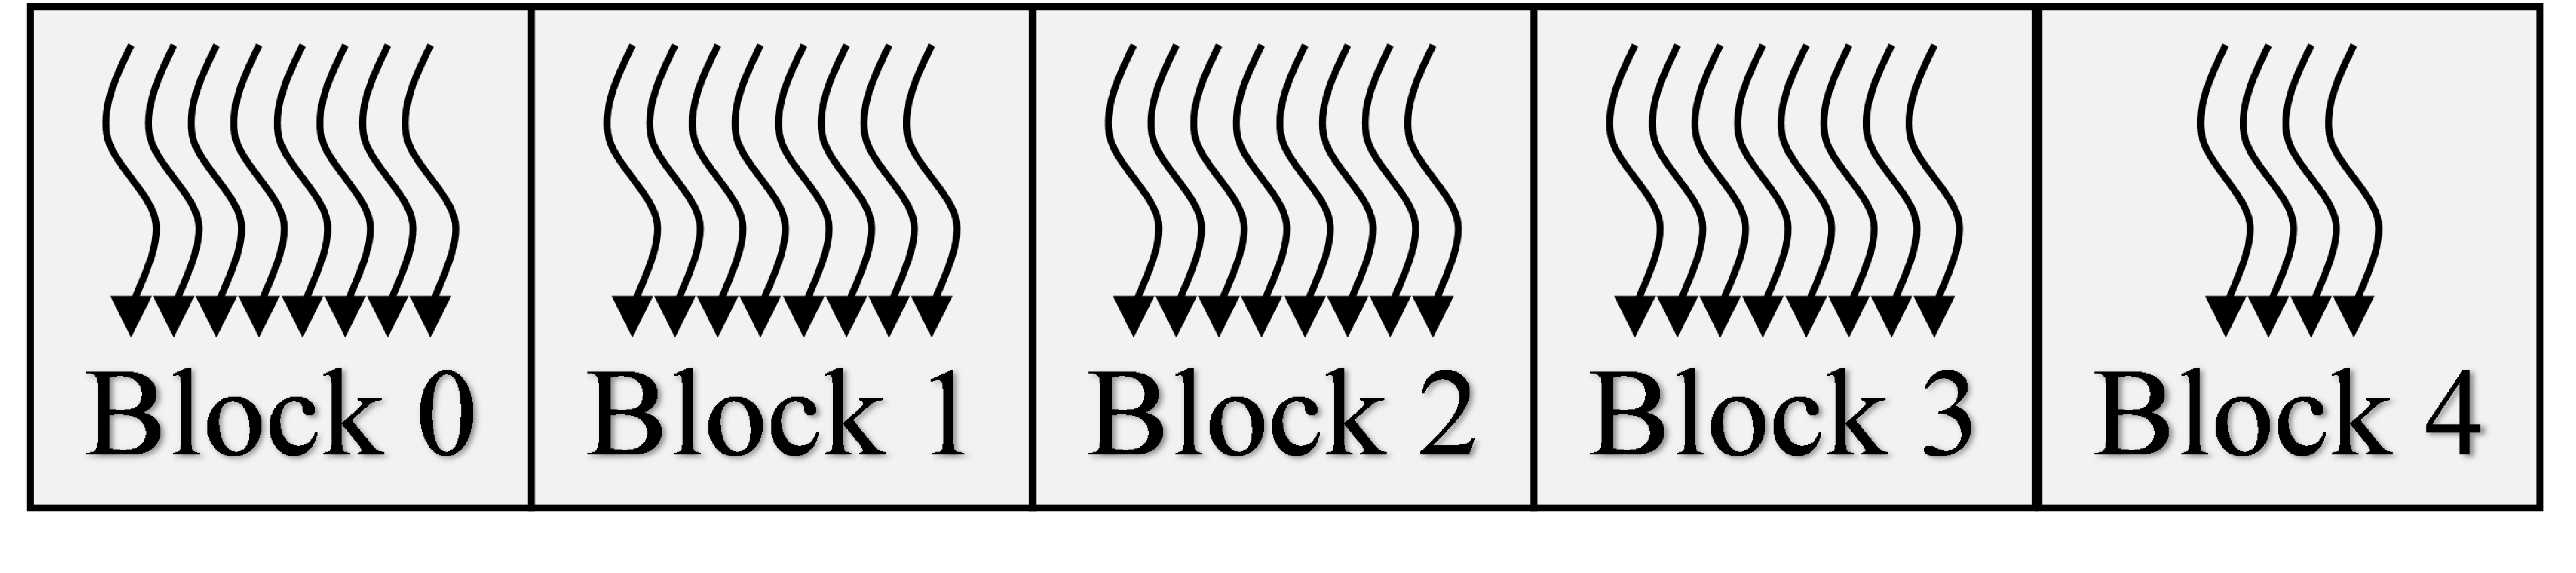
\includegraphics[width=5in/100*55]{figures/gpu_intro/threadsBlocks36.pdf}
	\caption{$36$ threads launched in $5$ thread blocks with $8$ threads per block with $4$ idle threads.}
	\label{fig:threadsBlocks36}
\end{figure}

\subsection{GPU Memory}
\label{sec:GPU_memory}
GPUs have plenty of computational resources but most GPU kernels are limited by memory bandwidth to feed the computational units.
GPU kernels execute faster if the kernel is designed to access memory efficiently rather than reducing the computational burden.
NVIDIA GPUs have many different types of memory to maximize speed and efficiency.

The fastest memory is private local memory,
in the form of Registers and L1 Cache/shared memory.
Local memory is fast but only kilobytes are available.
The slowest memory is public memory in the form of the L2 Cache and Global Memory.
Public memory is slow but gigabytes are available.
Figure \ref{fig:MemoryPyramid} shows the trade-off of memory speed and the size of different types of memory.
\begin{figure}
	\centering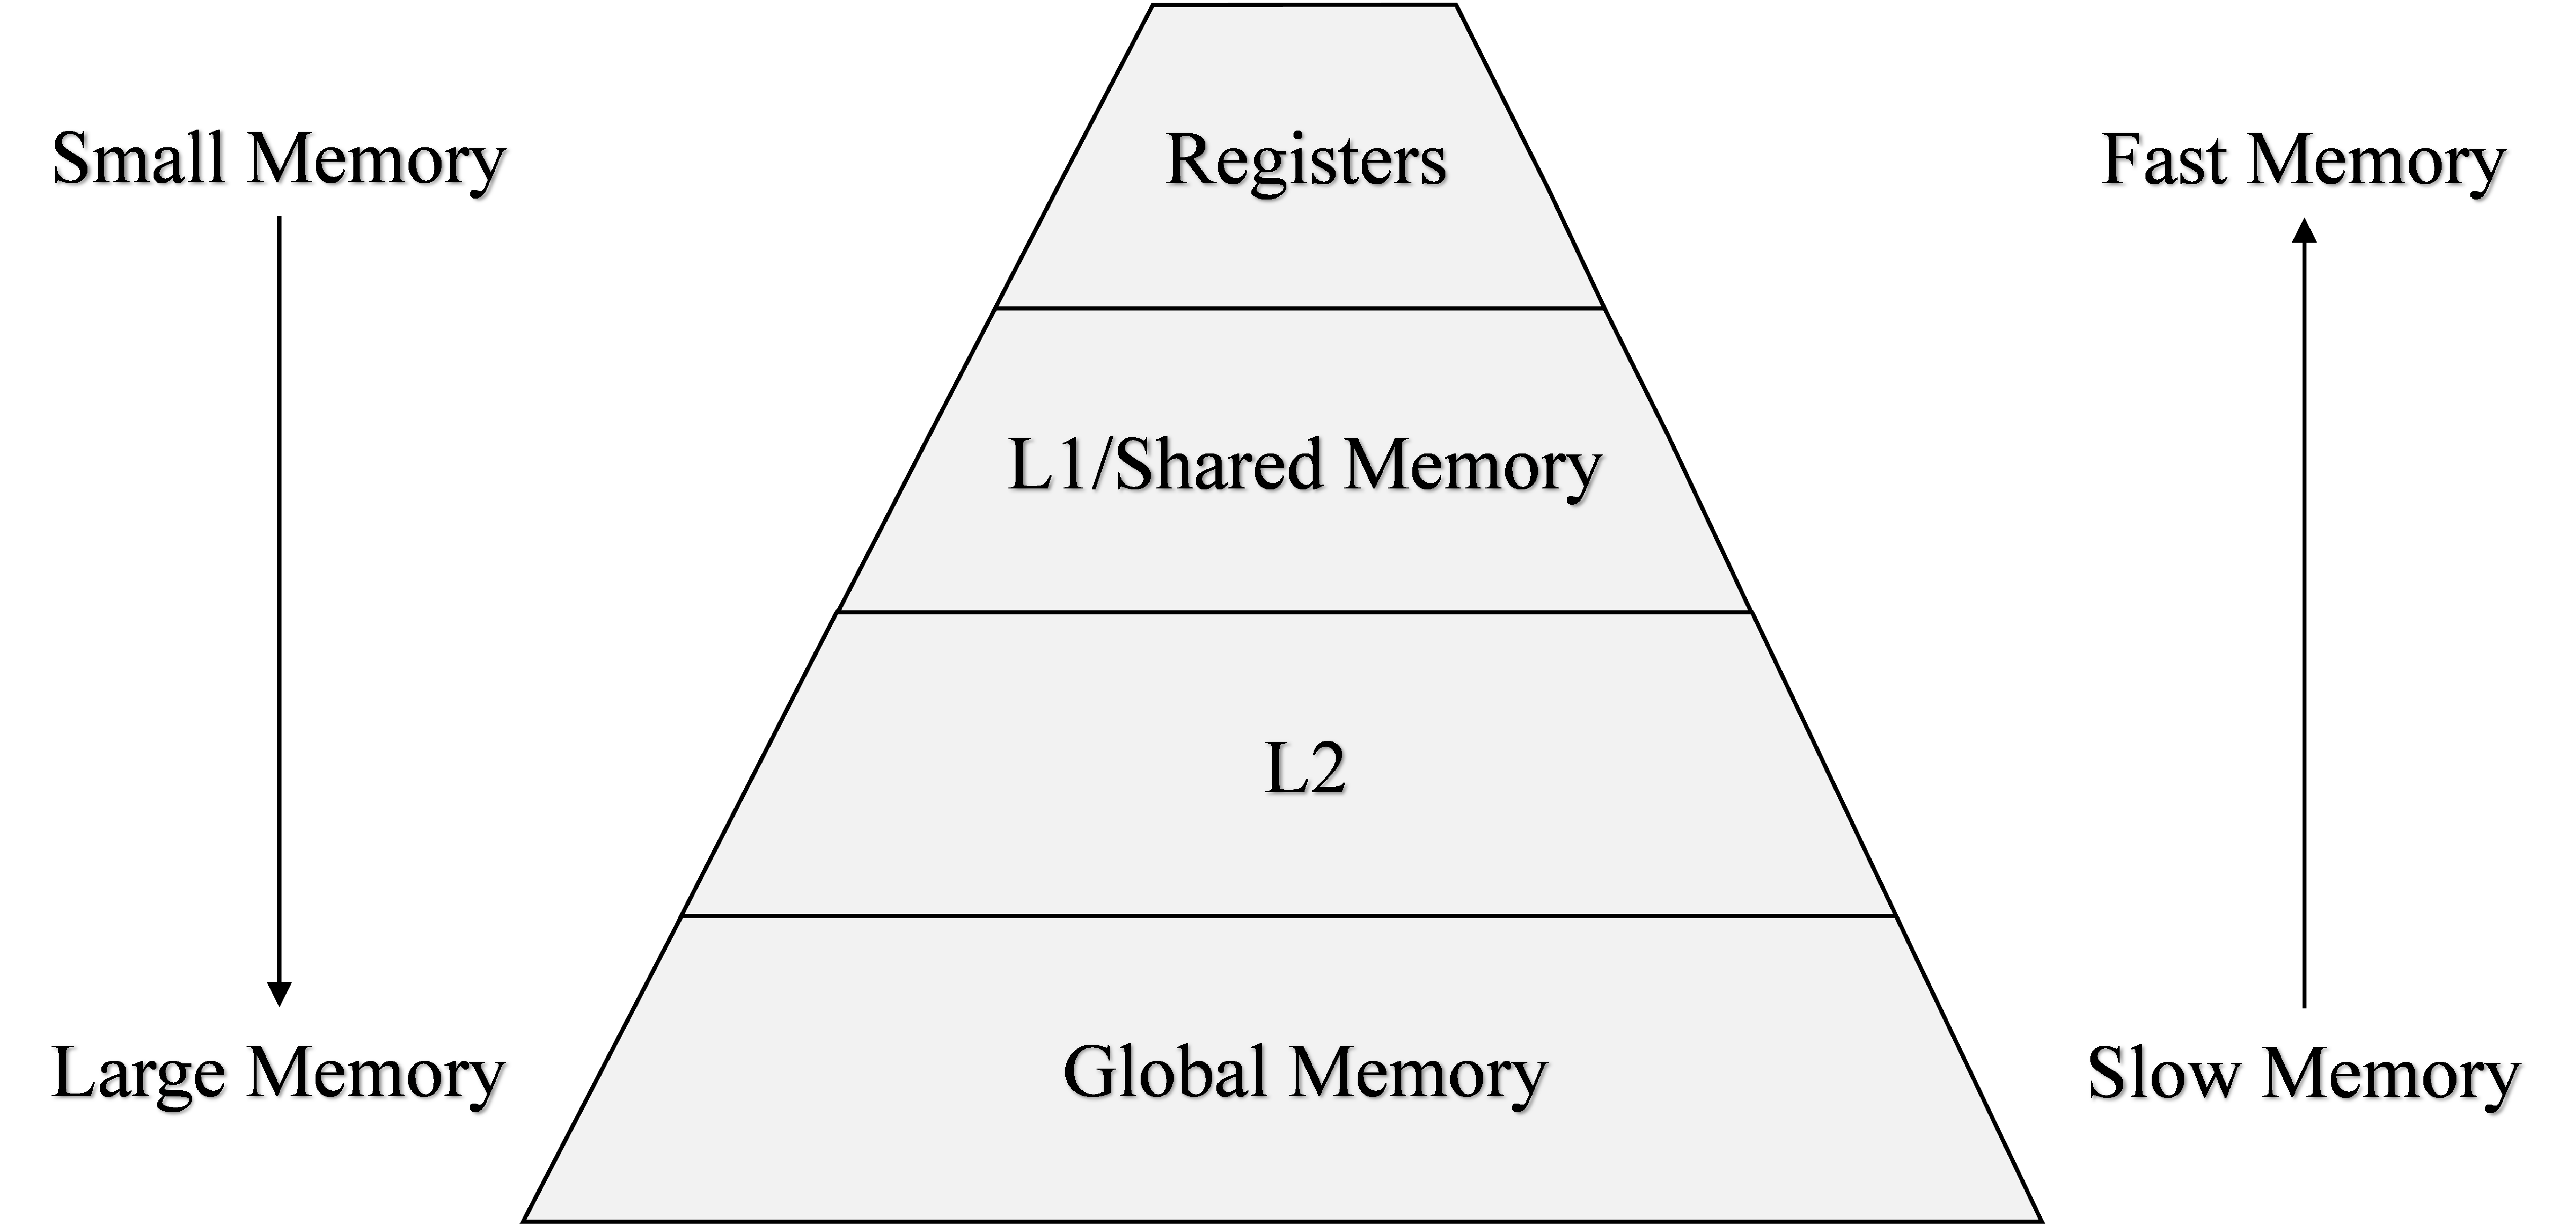
\includegraphics[width=8.36in/100*55]{figures/gpu_intro/MemoryPyramid.pdf}
	\caption{Diagram comparing memory size and speed. Global memory is massive but extremely slow. Registers are extremely fast but there are very few.}
	\label{fig:MemoryPyramid}
\end{figure}

Figure \ref{fig:GPUarch} shows a picture of the GPU hardware.
The solid boxes show that the L2 cache and Global Memory are physically located \textit{off} the GPU chip. 
The dashed box shows that Registers and L1 Cache/Shared Memory are physically located \textit{on} the GPU chip. 
A public access takes over 60 clock cycles because the memory is off chip. 
A local memory access is only a few clock cycles because the memory is on chip.
\begin{figure}
	\centering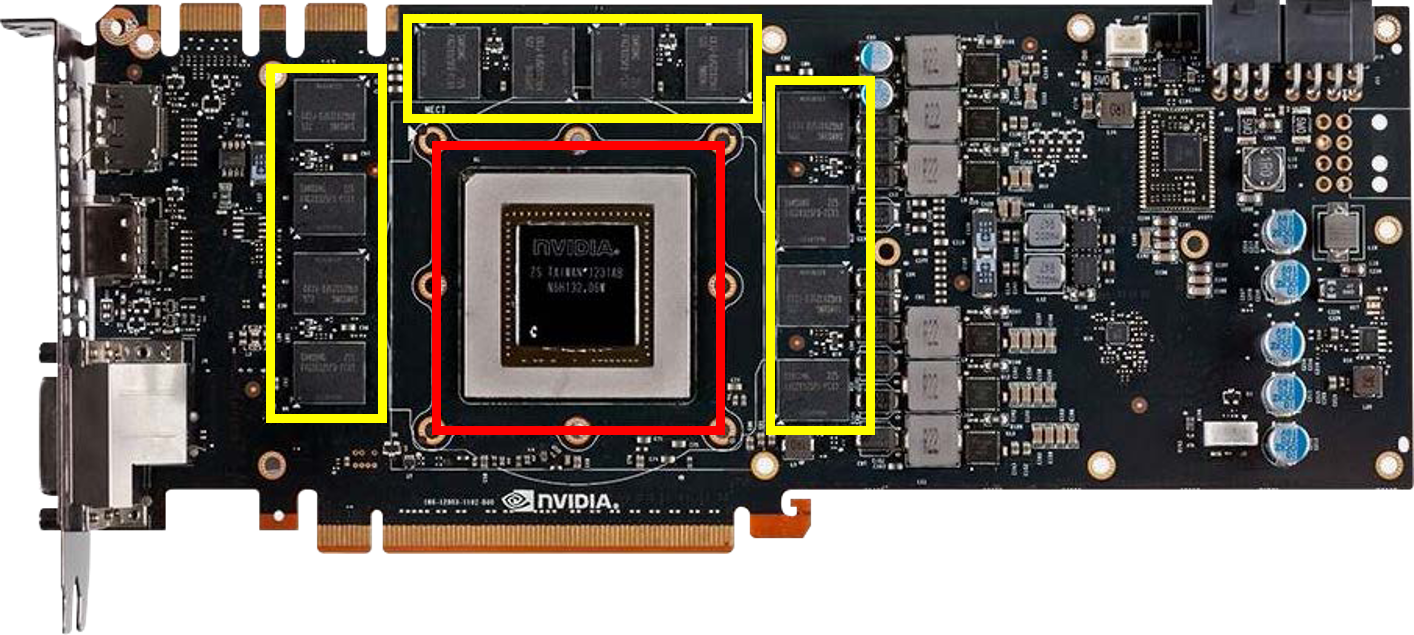
\includegraphics[width=\textwidth]{figures/gpu_intro/Kepler_box.png}
	\caption{Example of an NVIDIA GPU card. The GPU chip with registers and L1/shared memory is shown in the dashed box.	The L2 cache and global memory is shown off chip in the solid boxes.}
	\label{fig:GPUarch}
\end{figure}

Figure \ref{fig:fullGPUmemBlockDiagram} illustrates where each type of memory is located.
Threads have access to their own Registers and the L1 Cache.
Threads in a block can coordinate using shared memory because shared memory is private to the thread block.
All threads have access to the L2 Cache and Global Memory.
The figure also shows that thread blocks are assigned to streaming multiprocessors (SMs).
CUDA handles all the thread block assignments to SMs.
\begin{figure}
	\centering\includegraphics[width=9.83in/100*55]{figures/gpu_intro/fullGPUmemBlockDiagram.pdf}
	\caption{A block diagram where local, shared, and global memory is located. Each thread has private local memory. Each thread block has private shared memory. The GPU has global memory that all threads can access.}
	\label{fig:fullGPUmemBlockDiagram}
\end{figure}
Table \ref{tab:gpu-resources_jeffs} lists Telsa K40c and K20c resources.
\begin{table}
\caption{The resources available with three NVIDIA GPUs used in this thesis (1x Tesla K40c 2x Tesla K20c). Note that CUDA configures the size of the L1 cache needed.}
\begin{center}
\begin{tabular}{llll}
	\toprule
	Feature 			& Per			& Tesla K40c 	& Tesla K20c	\\ \midrule
	Global Memory 		& GPU			& 12 GB	 		& 5 GB			\\
	L2 Cache Size 		& GPU			& 1.6 GB		& 1.3 GB		\\
	Memory Bandwidth	& 				& 288 GB/s		& 208 GB/s		\\		
	Shared Memory 		& Thread Block	& 49 kB			& 49 kB			\\
	L1 Cache Size 		& Thread Block	& variable		& variable		\\
	Registers			& Thread Block	& 65536			& 65536			\\
	Maximum Threads		& Thread Block	& 1024			& 1024			\\
	CUDA Cores 			& GPU			& 2880 			& 2496 			\\
	Base Core Clock 	&				& 745 MHz 		& 732 MHz		\\ \bottomrule
\end{tabular}
\end{center}
\label{tab:gpu-resources_jeffs}
\end{table}

\subsection{Thread Optimization}
Most resources listed in Table \ref{tab:gpu-resources_jeffs} show how much memory per thread block is available. 
The number of threads per block and the amount of resources available have an inverse relationship.
Threads have very little memory resources available if a GPU kernel launches 1024 threads per block.
Threads have a lot of memory resources available if a GPU kernel launches 32 threads per block.
This section shows that finding the optimum number of threads per block can dramatically speed up GPU kernels.

Improving memory accesses should always be the first optimization when a GPU kernel needs to be faster.
The next step is to find the optimal number of threads per block to launch.
Knowing the perfect number of threads per block to launch is challenging to calculate.
Fortunately, the maximum number of possible threads per block is $1024$ in the Tesla K40c and K20c GPUs.
Listing \ref{code:threadTiming} shows a simple test program that measures GPU kernel execution time while varying the number of possible threads per block.
The number of threads per block with the fastest computation time is the optimal number of threads per block for that specific GPU kernel.

\singlespacing
\clearpage
\begin{lstlisting}[style=myCUDAstyle,caption={Code snippet for thread optimization.},label={code:threadTiming}]
float milliseconds_opt = pow(2,10); // initiaize to "big" number
int T_B_opt;
int minNumTotalThreads = pow(2,20); // set to minimum number of required threads
for(int T_B = 1; T_B<=1024; T_B++){
	int B = minNumTotalThreads/T_B;
	if(minNumTotalThreads % T_B > 0)
		B++;
	cudaEvent_t start, stop;
	cudaEventCreate(&start);
	cudaEventCreate(&stop);
	cudaEventRecord(start);
	
	GPUkernel<<<B, T_B>>>(dev_vec0, dev_vec1);
	
	cudaEventRecord(stop);
	cudaEventSynchronize(stop);
	float milliseconds = 0;
	cudaEventElapsedTime(&milliseconds, start, stop);
	cudaEventDestroy(start);
	cudaEventDestroy(stop);
	if(milliseconds<milliseconds_opt){
		milliseconds_opt = milliseconds;
		T_B_opt = T_B;
	}
}
cout << "Optimal Threads Per Block " << T_B_opt << endl
cout << "Optimal Execution Time    " << milliseconds_opt << endl;
\end{lstlisting}
\doublespacing

Most of the time the optimal number of threads per block is a multiple of $32$ this is because
at the lowest level of architecture, GPUs perform computations in \textit{warps}.
Warps are groups of $32$ threads that perform every computation together in lock step.
If the number of threads per block is not a multiple of $32$, some threads in a warp are idle and the GPU has unused computational resources.

Figure \ref{fig:ConvGPU_shared_12672_186taps} shows the execution time of an example GPU kernel.
The optimal execution time is $0.1078$ ms at the optimal $96$ threads per block.
By simply adjusting the number of threads per block, the execution time of this example kernel can be reduced by 2.

Adjusting the number of threads per block does not always dramatically reduce execution time.
Figure \ref{fig:ConvGPU_global_12672_186taps} shows the execution time for another GPU kernel with varying threads per block.
The execution time of this example kernel can be reduced by 1.12 by launching $560$ threads per block.
\begin{figure}
	\centering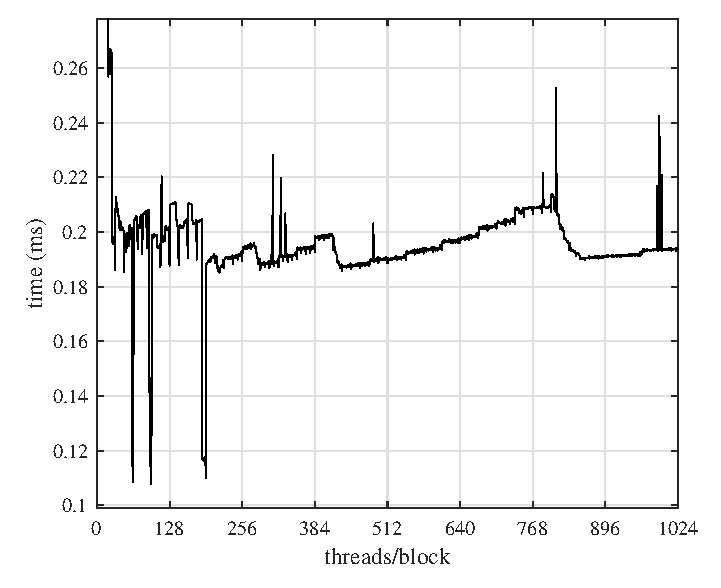
\includegraphics[width=5in]{figures/gpu_intro/ConvGPU_shared_12672_186taps.eps}
	\caption{Plot showing how execution time is affected by changing the number of threads per block.
	The optimal execution time for an example GPU kernel is $0.1078$ ms at the optimal $96$ threads per block.}
	\label{fig:ConvGPU_shared_12672_186taps}
\end{figure}
\begin{figure}
	\centering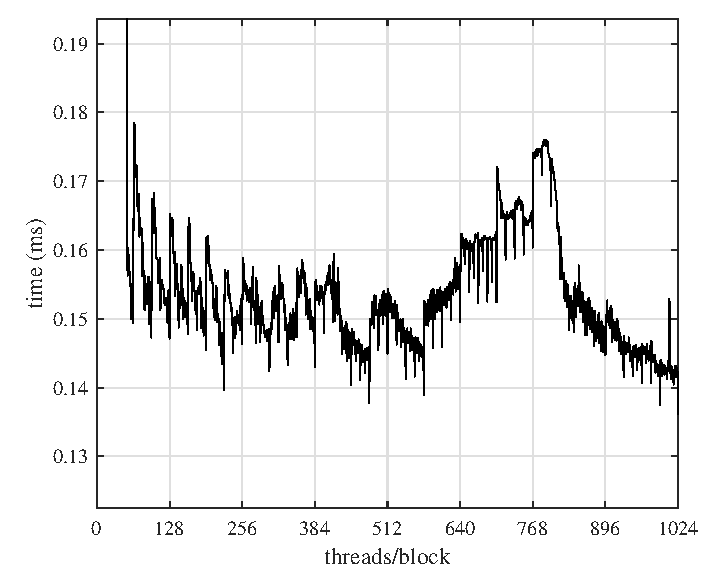
\includegraphics[width=5in]{figures/gpu_intro/ConvGPU_global_12672_186taps.eps}
	\caption{Plot showing the number of threads per block doesn't always drastically affect execution time.}
	\label{fig:ConvGPU_global_12672_186taps}
\end{figure}

While designing a custom GPU kernel to obtain a major speed up is satisfying,
CUDA has optimized GPU libraries that are extremely useful and efficient with exceptional documentation.
The CUDA libraries are written by NVIDIA engineers to maximize the performance of NVIDIA GPUs.
The libraries explained in this thesis include cuFFT, cuBLAS and cuSolverSp.

\subsection{CPU and GPU Pipelining}
While GPU kernels execute physically on the GPU, the GPU only executes instructions received from the host CPU.
The CPU is idle while it waits for GPU kernels to execute.
To introduce CPU and GPU pipelining, the CPU can be pipelined by performing other operations while waiting for the GPU to finish executing kernels.

A basic CPU GPU program with no pipelining is shown in Listing \ref{code:noPipe}.
The CPU acquires data from myADC on Line 5.
After the CPU takes time to acquire data, the data is copied from the host (CPU) to the device (GPU) on line 8.
The data is processed on the GPU once then the result is copied back to the device to host on line 9 and 10.
The cudaDeviceSynchronize function on line 13 blocks CPU until all GPU instructions are finished executing.
Note that the CPU is blocked during any host to device or device to host transfer.
Acquiring and copying data takes processing time on the CPU and GPU.
Figure \ref{fig:concurrentCPU_blocking} shows a block diagram of what is happening on the CPU and GPU in Listing \ref{code:noPipe} (end of the section).
The GPU is idle while the CPU is acquiring data and the CPU is idle while the GPU is processing.
\begin{figure}
	\centering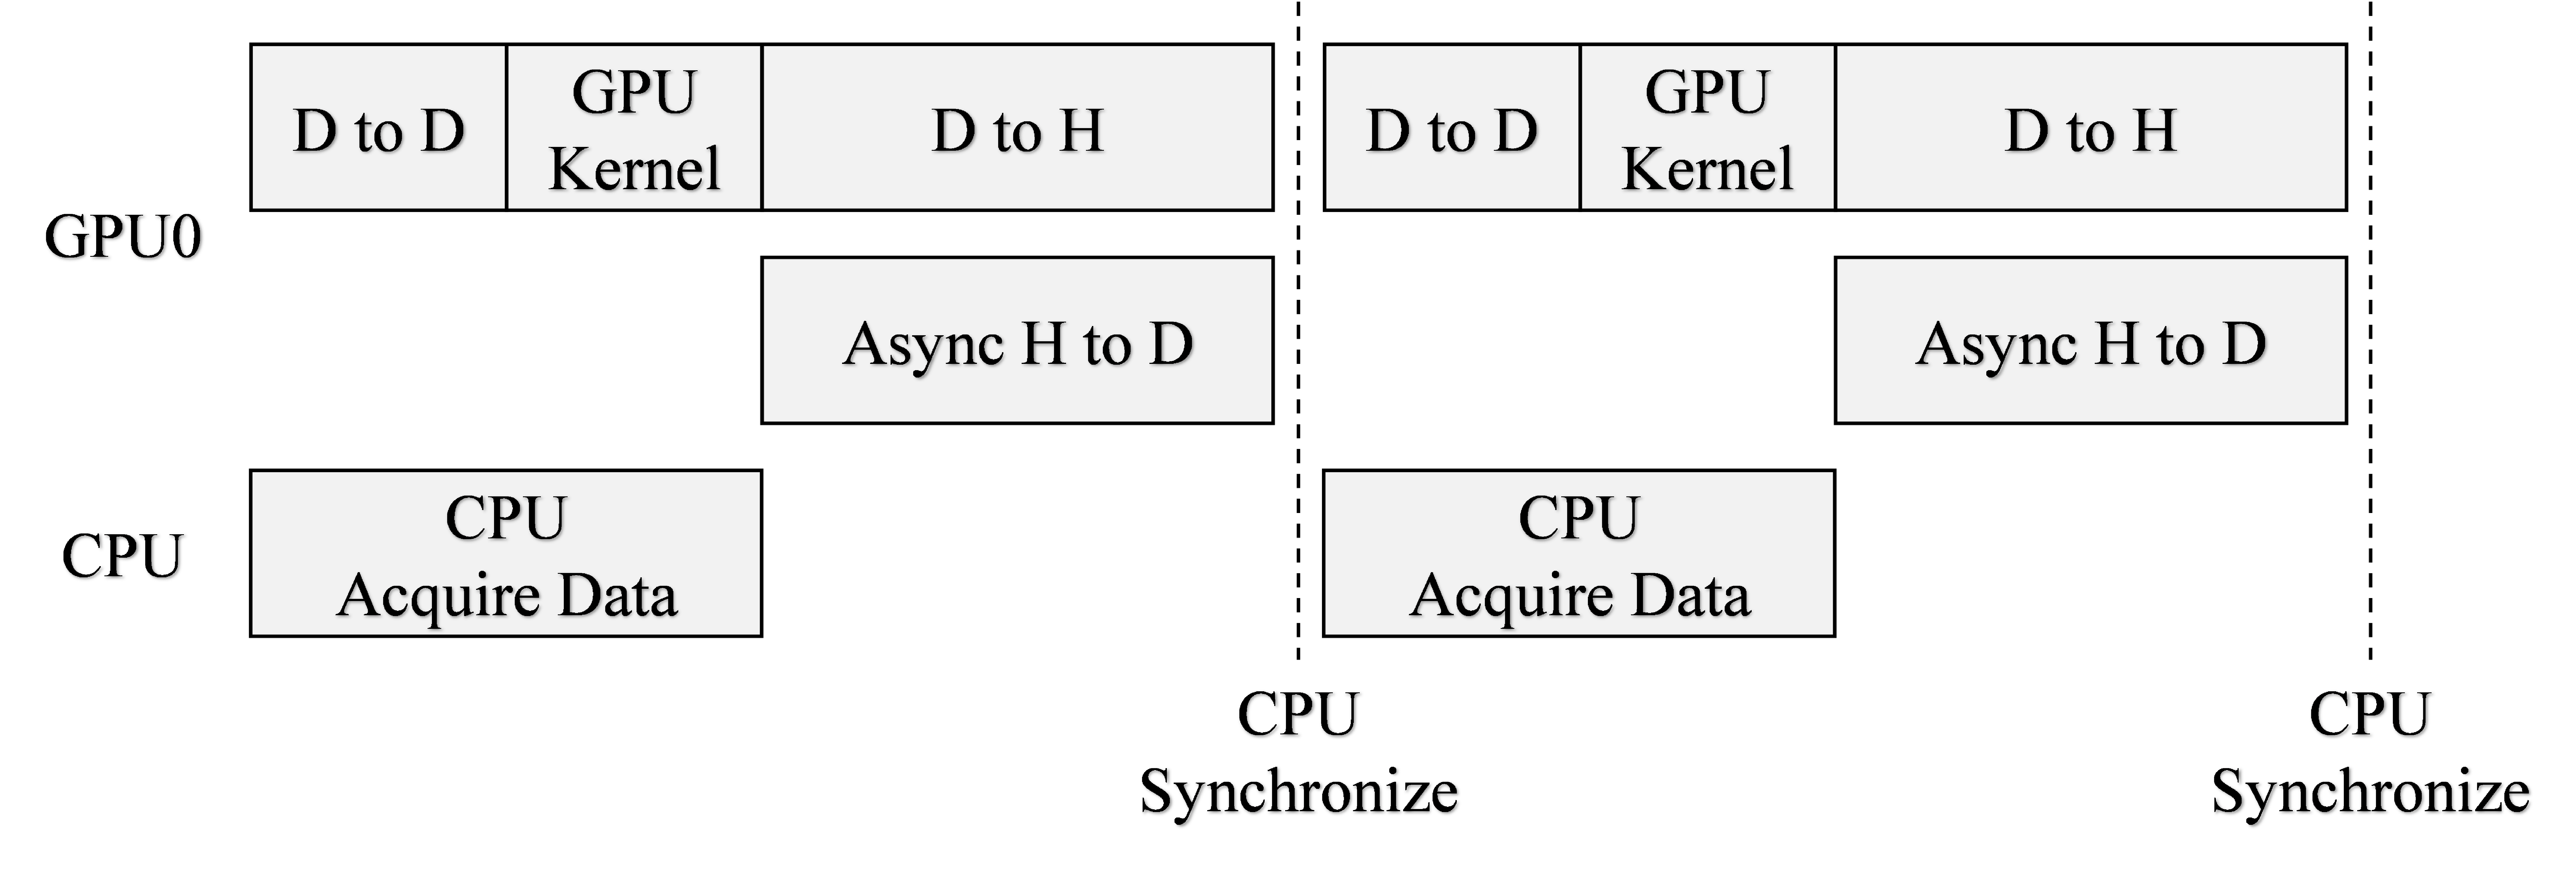
\includegraphics[width=8.77in/100*55]{figures/gpu_intro/concurrentCPU_blocking.pdf}
	\caption{The typical approach of CPU and GPU operations. This block diagram shows the profile of Listing \ref{code:noPipe}.}
	\label{fig:concurrentCPU_blocking}
\end{figure}

Listing \ref{code:pipe} (end of the section) shows how to CPU and GPU operations can be pipelined.
Assuming data is already on the GPU from a prior computation, the CPU gives processing instructions to the GPU then acquires data.
The CPU then does an asynchronous data transfer to a temporary vector on the GPU.
The GPU first performs a device to device transfer from the temporary vector.
The GPU then runs the GPUkernel and transfers the result to the host.
Note that device to device transfers do not block the CPU.
This system suffers a full cycle latency.
\begin{figure}
	\centering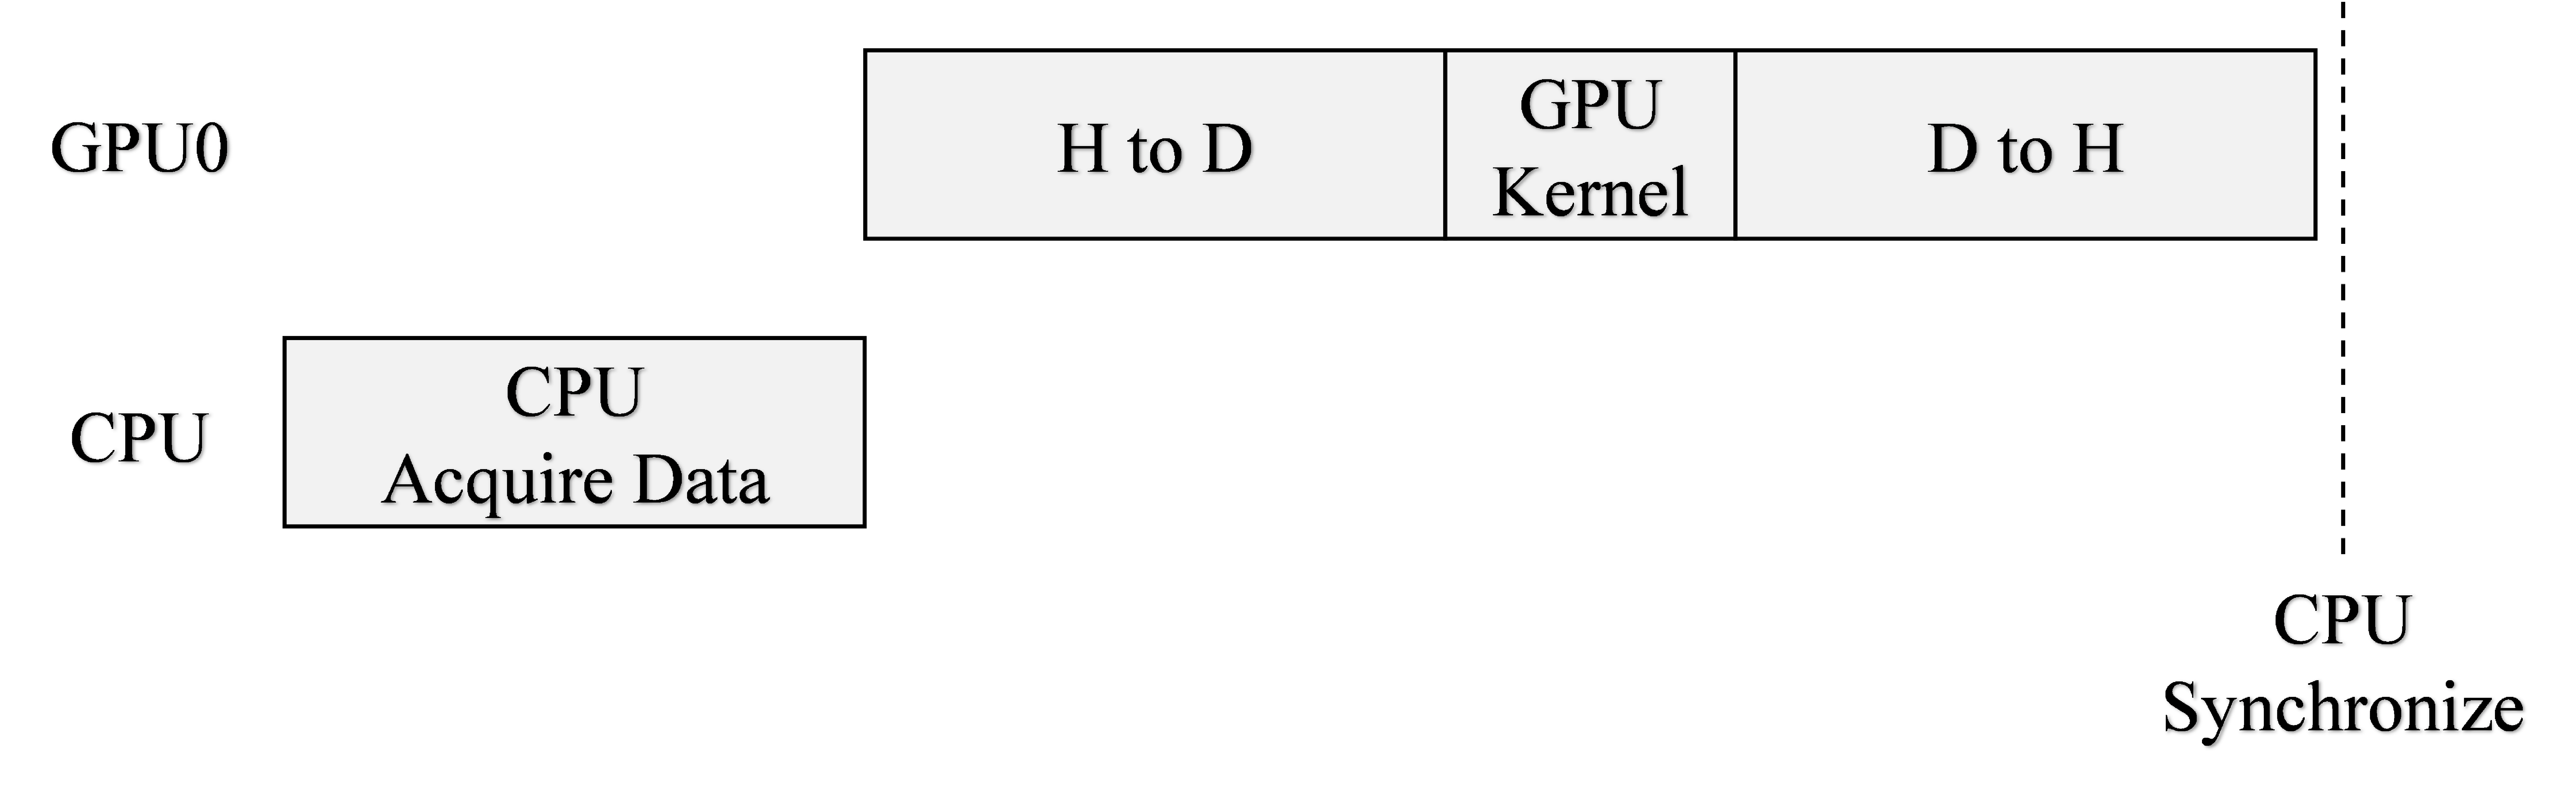
\includegraphics[width=9.97in/100*55]{figures/gpu_intro/concurrentCPU_nonBlocking.pdf}
	\caption{GPU and CPU operations can be pipelined. This block diagram shows a Profile of Listing \ref{code:pipe}.}
	\label{fig:concurrentCPU_nonBlocking}
\end{figure}

Pipelineing can be extended to multiple GPUs for even more throughput but only suffer latency of copying memory to one GPU.
Figure \ref{fig:concurrentCPU_nonBlocking_multiGPU} shows a block diagram of how three GPUs can be pipelined.
A strong understanding of the full system is required to pipeline at this level.
\begin{figure}
	\centering\includegraphics[width=11.4in/100*55]{figures/gpu_intro/concurrentCPU_nonBlocking_multiGPU.pdf}
	\caption{A block diagram of pipelining a CPU with three GPUs.}
	\label{fig:concurrentCPU_nonBlocking_multiGPU}
\end{figure}

\singlespacing
\clearpage
\begin{lstlisting}[style=myCUDAstyle,caption={Example code Simple example of the CPU acquiring data from myADC, copying from host to device, processing data on the device then copying from device to host. No processing occurs on device while CPU is acquiring data.},label={code:noPipe}]
int main()
{
	...
	// CPU Acuire Data
	myADC.acquire(vec);
	
	// Launch instructions on GPU 
	cudaMemcpy(dev_vec0, vec,      numBytes, cudaMemcpyHostToDevice);
	GPUkernel<<<1, N>>>(dev_vec0);
	cudaMemcpy(vec,      dev_vec0, numBytes, cudaMemcpyDeviceToHost);
	
	// Synchronize CPU with GPU
	cudaDeviceSynchronize();
	...
}
\end{lstlisting}
\doublespacing
\singlespacing
\begin{lstlisting}[style=myCUDAstyle,caption={Example code Simple of the CPU acquiring data from myADC, copying from host to device, processing data on the device then copying from device to host. No processing occurs on device while CPU is acquiring data.},label={code:pipe}]
int main()
{
	...
	// Launch instructions on GPU 
	cudaMemcpy(dev_vec, dev_temp, numBytes, cudaMemcpyDeviceToDevice);
	GPUkernel<<<N, M>>>(dev_vec);
	cudaMemcpy(vec,     dev_vec,  numBytes, cudaMemcpyDeviceToHost);
	
	// CPU Acuire Data
	myADC.acquire(vec);
	cudaMemcpyAsync(dev_temp, vec, numBytes, cudaMemcpyHostToDevice);
	
	// Synchronize CPU with GPU
	cudaDeviceSynchronize();
	...
	
	...
	// Launch instructions on GPU 
	cudaMemcpy(dev_vec, dev_temp, numBytes, cudaMemcpyDeviceToDevice);
	GPUkernel<<<N, M>>>(dev_vec);
	cudaMemcpy(vec,     dev_vec,  numBytes, cudaMemcpyDeviceToHost);
	
	// CPU Acuire Data
	myADC.acquire(vec);
	cudaMemcpyAsync(dev_temp, vec, numBytes, cudaMemcpyHostToDevice);
	
	// Synchronize CPU with GPU
	cudaDeviceSynchronize();
	...
}
\end{lstlisting}
\doublespacing

\clearpage
\section{GPU Convolution}
\label{chap:gpu_convolution}
Convolution is one of the most important tools in digital signal processing.
The PAQ system explained uses convolution up to 26 times per packet, depending on the number of CMA iterations.
If convolution execution time can be reduced by 10 ms, the full system execution time can reduced by 260 ms.
This section will use the following notation: 
\begin{itemize}
\item The signal $\mathbf{x}$ is a vector of $N$ complex samples indexed by $x(n)$ where $0 \leq \leq N-1$.
\item The filter $\mathbf{h}$ is a vector of $L$ complex samples indexed by $h(n)$ where $0 \leq \leq L-1$.
\item The filtered signal $\mathbf{y}$ is a vector resulting from the convolution of $\mathbf{x}$ and $\mathbf{h}$. $\mathbf{y}$ is $C = N + L -1$ complex samples and is indexed by $y(n)$ where $0 \leq n \leq C-1$.
\item The forward Fast Fourier Transform (FFT) of the vector $\mathbf{x}$ is denoted $\mathscr{F}(\mathbf{x})$.
\item The inverse Fast Fourier Transform (IFFT) of the vector $\mathbf{x}$ is denoted $\mathscr{F}^{-1}(\mathbf{x})$.
\end{itemize}

Discrete time convolution applies the filter $\mathbf{h}$ to the signal $\mathbf{x}$ resulting in the filter signal $\mathbf{y}$.
Convolution in the time domain is
\begin{equation}
y(n) = \sum^{L-1}_{m=0} x(m) h(n-m)
  \label{eq:simple_conv_time}
\end{equation}
and the frequency domain is
\begin{equation}
\mathbf{y} = \mathscr{F}^{-1}(\mathscr{F}(\mathbf{x})\times\mathscr{F}(\mathbf{h})).
  \label{eq:simple_conv_freq}
\end{equation}
Figure \ref{fig:freq_time_block} shows block diagrams for time-domain and frequency domain convolution.
\begin{figure}
	\centering\includegraphics[width=10.28in/100*55]{figures/gpu_convolution/convBlock.pdf}
	\caption{Block diagrams showing time-domain convolution and frequency-domain convolution.}
	\label{fig:freq_time_block}
\end{figure}
This section will show:
\begin{itemize}
\item GPU convolution is faster than CPU convolution with large data sets using execution time as a metric.
\item GPU convolution execution time is dependent more on memory access than floating point operations.
\item Performing batched GPU convolution invokes more parallelism and decreases execution time per batch.
\item Batched GPU frequency-domain convolution executes faster than batched GPU time-domain convolution.
\end{itemize}

\subsection{Floating Point Operation Comparison}
Traditionally the number of floating point operations (flops) is used to estimate how computationally intense an algorithm is. 
Each complex multiplication  
\begin{equation}
(A+jB)\times(C+jD) = (AC-BD)+j(AD+BC)
\end{equation}
requires $6$ flops, $4$ multiplications and $2$ additions/subtractions.
Output elements of $\mathbf{y}$ in Equation \eqref{eq:simple_conv_time} requires $8L = (6+2)L$ flops, $2$ extra flops are required for each summand.
The time-domain convolution requires
\begin{equation}
8LC \text{ flops}
\label{eq:flops_time_domain_conv}
\end{equation}
where $C=N+L-1$ is the length of the convolution result.

To leverage the Cooley-Tukey radix 2 Fast Fourier Transform (FFT) in frequency-domain convolution, common practice is to compute the $M$ point FFT where $M = 2^u$ and $u = {\left\lceil \log_2{\left(C\right)}  \right\rceil}$.
Both the CPU based Fastest Fourier Transform in the West (FFTW) library and the NVIDIA GPU cuFFT library use the Cooley-Tukey radix 2 FFT.
Each FFT or IFFT requires $5M\log_2(M)$ flops \cite{FFTW:2017,cooley1965algorithm}.
As shown by Equation \eqref{eq:simple_conv_freq}, frequency-domain convolution requires 
\begin{equation}
3\times5M\log_2(M)+6M \text{ flops}
\label{eq:flops_freq_domain_conv}
\end{equation}
from $3$ FFTs and $M$ point-to-point multiplications.

Sections \ref{sec:hardware} and \ref{sec:oqpsk_detector} show the PAQ system has one signal length, $N = \Lpkt = 12672$ samples and two filter lengths $L = L_\text{df} = 23$ and $L = L_\text{eq} = 186$.
Figures \ref{fig:Theory186Tap_flops} through \ref{fig:Theory12672signal_flops} compare the number of flops required for time-domain and frequency-domain convolution.
The figures compare flops by fixing the signal length with variable filter length or visa versa.
These figures show applying a $186$ tap filter to a $12672$ sample signal requires less flops in the frequency domain and
applying a $23$ tap filter to a $12672$ sample signal requires less flops in the time domain.
\begin{figure}
	\centering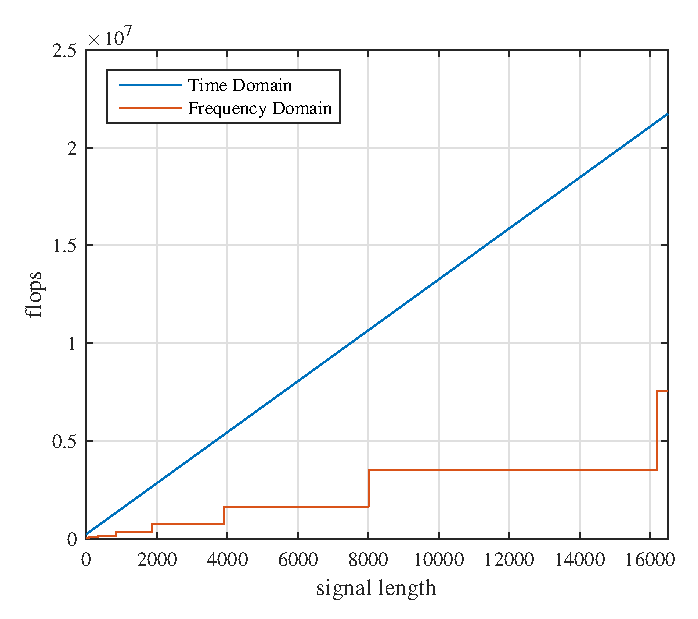
\includegraphics[width=5in]{figures/gpu_intro/Theory186Tap_flops.eps}
	\caption{Comparison of number of floating point operations (flops) required to convolve a variable length complex signal with a $186$ tap complex filter.}
	\label{fig:Theory186Tap_flops}
\end{figure}
\begin{figure}
	\centering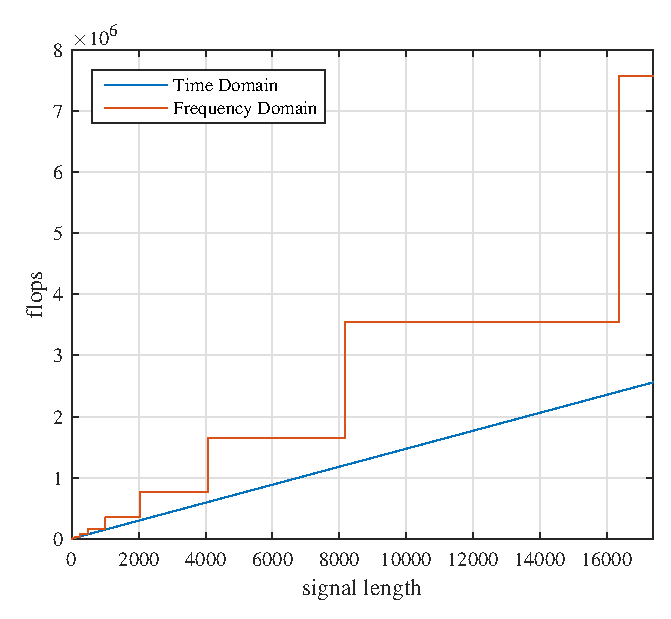
\includegraphics[width=5in]{figures/gpu_intro/Theory21Tap_flops.eps}
	\caption{Comparison of number of floating point operations (flops) required to convolve a variable length complex signal with a $23$ tap complex filter.}
	\label{fig:Theory21Tap_flops}
\end{figure}
\begin{figure} 
	\centering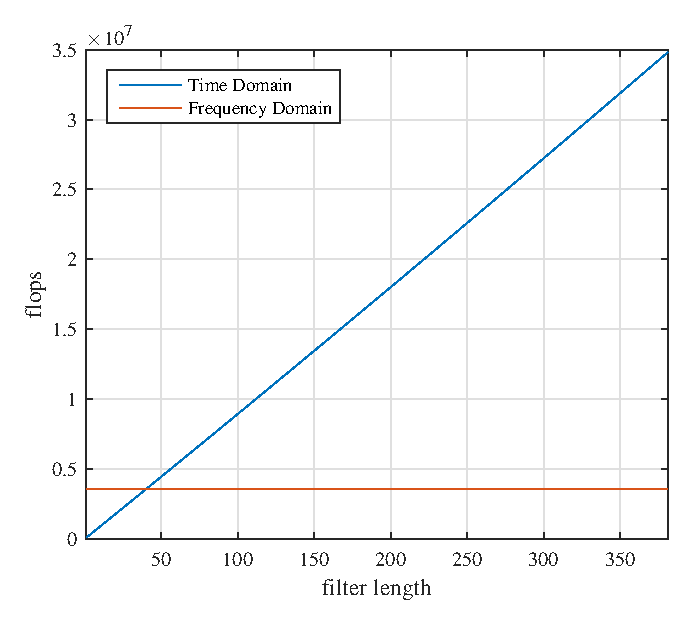
\includegraphics[width=5in]{figures/gpu_intro/Theory12672signal_flops.eps}
	\caption{Comparison of number of floating point operations (flops) required to convolve a $12672$ sample complex signal with a variable length tap complex filter.}
	\label{fig:Theory12672signal_flops}
\end{figure}

\subsection{CPU and GPU Single convolution using batch processing Comparison}
\label{sec:cuda_convolution_single}
This section will show GPU convolution execution time is dependent more on memory access than the number of required floating point operations while CPU convolution execution time is dependent on the number of floating point operations.
To illustrate these points, the execution time of the code in Listing \ref{code:convFun} (at the end of the chapter) was measured.
The code implements convolution five different ways:
\begin{itemize}
  \item time-domain convolution in a CPU
  \item frequency-domain convolution in a CPU using the FFTW library
  \item time-domain convolution in a GPU using global memory
  \item time-domain convolution in a GPU using shared memory
  \item frequency-domain convolution in a GPU using the cuFFT library
\end{itemize}

The three time-domain convolution implementations compute \eqref{eq:simple_conv_time} directly.
The two \newline frequency-domain convolution implementations compute \eqref{eq:simple_conv_freq} using the CPU FFTW library and the GPU based cuFFT library.
The cuFFT library uses global memory and shared memory to be as fast and efficient as possible.
For a given signal and filter length, a good CUDA programmer can make an educated guess on which algorithm is faster.
There is no clear conclusion until all the algorithms have been implemented and measured.

%The CPU implements Equation \eqref{eq:simple_conv_time} in ConvCPU directly on line $209$ using a function from lines $11$ to $34$.
%The CPU implements Equation \eqref{eq:simple_conv_freq} using the FFTW library on lines $214$ to $258$.
%
%The GPU implements time-domain convolution using global memory in lines $268$ to $277$.
%The GPU kernel ConvGPU on lines $36$ to $64$ is a parallel version of ConvCPU.
%ConvGPU performs time-domain convolution by fetching every element of the signal and filter from global memory.
%
%The GPU implements time-domain convolution using shared memory in lines $283$ to $292$.
%The GPU kernel ConvGPUshared on lines $67$ to $101$ is nearly identical to ConvGPU.
%Threads accessing the same elements of the filter in global memory can be a waste of valuable clock cycles.
%ConvGPUshared pays and initial price on lines $72$ to $76$ to move $L_\text{h}$ filter coefficients from off chip global memory to the on chip shared memory.
%Finally, the GPU implements frequency-domain convolution using the cuFFT library on lines $298$ to $326$.
%
%The questions are:
%Do flops have a direct relationship to execution time on CPUs? 
%Do flops have a direct relationship to execution time on GPUs? 
%When is the initial cost to use shared memory worth it?
%When should convolution be done in the frequency domain?
%
%The short answer to all of the questions is: GPU execution time depend on the signal length, filter length, CPU, GPU and memory.
%A good CUDA programmer can make an educated guess on which algorithm may be faster in the GPU, but until all the algorithms have been implemented and timed, there is no definite answer.

All the memory transfers to and from the GPU were timed for a fair comparison of GPU to CPU execution time.
Table \ref{tab:CPUvsGPUtimingTable} shows how the execution time was measured for each convolution implementation.
\begin{table}
\caption{Defining start and stop lines for timing comparison in Listing \ref{code:convFun}.}
\begin{center}
\begin{tabular}{llll}
	\toprule
	Algorithm 				& Function		& Start Line	& Stop  Line		\\ \midrule
	CPU time domain 		& ConvCPU 		& 208			& 210 				\\
	CPU frequency domain 	& FFTW 			& 213			& 259 				\\
	GPU time domain global 	& ConvGPU 		& 267			& 278				\\
	GPU time domain shared 	& ConvGPUshared & 282			& 293				\\
	GPU frequency domain 	& cuFFT			& 301			& 327				\\ 
	\bottomrule
\end{tabular}
\end{center}
\label{tab:CPUvsGPUtimingTable}
\end{table}
Figures \ref{fig:CPUvsGPU_1batch_186taps_varySignal_noMin} through \ref{fig:CPUvsGPU_1batch_12672signal_varyFilter} compare execution time of the five different convolution implementations by fixing the filter length with variable signal length or visa versa.
Sub-windows emphasize points that are of interest to the PAQ system.
The variations in the time-domain CPU execution times are du to the claims on the host CPU resources by the operating system.
To clean up the time samples, local minimums were found in windows ranging from 3 to 15 samples.
The smallest windows possible were used to produce the results.
\begin{figure}
	\centering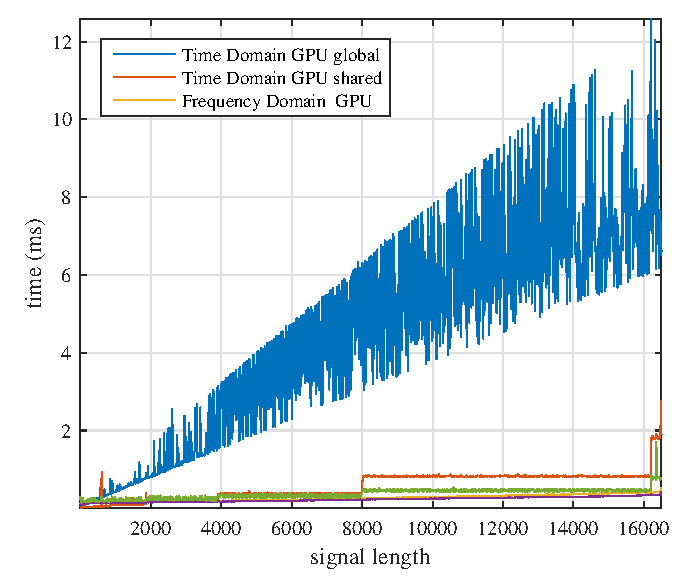
\includegraphics[width=5in]{figures/gpu_intro/CPUvsGPU_1batch_186taps_varySignal_noMin.eps}
	\caption{Comparison of a complex convolution on CPU and GPU. The signal length is variable and the filter is fixed at $186$ taps. The comparison is messy with out lower bounding.}
	\label{fig:CPUvsGPU_1batch_186taps_varySignal_noMin}
\end{figure}
\begin{figure}
	\centering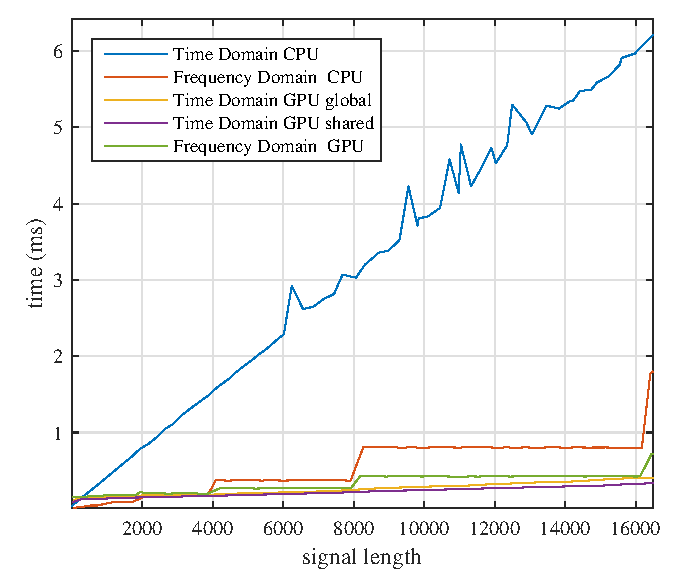
\includegraphics[width=5in]{figures/gpu_intro/CPUvsGPU_1batch_186taps_varySignal.eps}
	\caption{Comparison of a complex convolution on CPU and GPU. The signal length is variable and the filter is fixed at $186$ taps. A lower bound was applied by searching for a local minimums in 15 sample width windows.}
	\label{fig:CPUvsGPU_1batch_186taps_varySignal}
\end{figure}
\begin{figure}
	\centering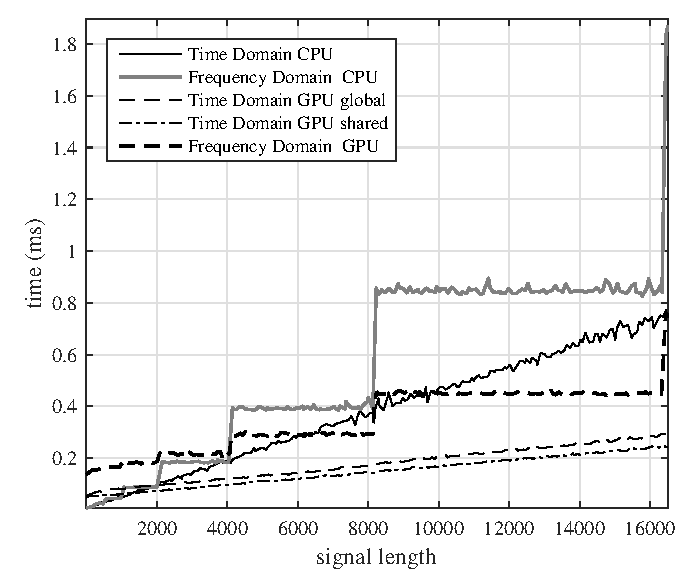
\includegraphics[width=5in]{figures/gpu_intro/CPUvsGPU_1batch_21taps_varySignal.eps}
	\caption{Comparison of a complex convolution on CPU and GPU. The signal length is variable and the filter is fixed at $23$ taps. A lower bound was applied by searching for a local minimums in 5 sample width windows.}
	\label{fig:CPUvsGPU_1batch_21taps_varySignal}
\end{figure}
\begin{figure}
	\centering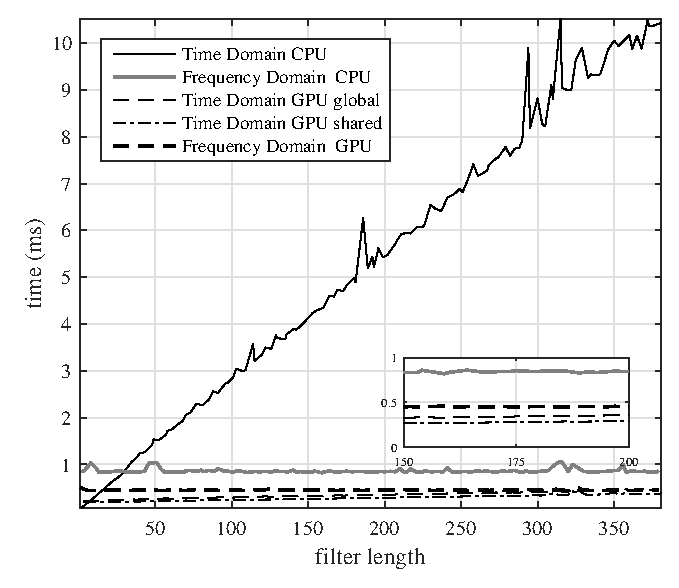
\includegraphics[width=5in]{figures/gpu_intro/CPUvsGPU_1batch_12672signal_varyFilter.eps}
	\caption{Comparison of a complex convolution on CPU and GPU. The filter length is variable and the signal is fixed at $12672$ samples. A lower bound was applied by searching for a local minimums in 3 sample width windows.}
	\label{fig:CPUvsGPU_1batch_12672signal_varyFilter}
\end{figure}

Comparing Figures \ref{fig:CPUvsGPU_1batch_186taps_varySignal} through \ref{fig:CPUvsGPU_1batch_12672signal_varyFilter}
to Figures \ref{fig:Theory186Tap_flops} through
\ref{fig:Theory12672signal_flops} 
shows
CPU and GPU convolution have the same structure that the number of flops predicted except GPU convolution is not affected as much by varied signal or filter lengths.
The convolution execution time comparison demonstrates the observation that most GPU kernels execution time is limited by memory bandwidth not computational resources.
Tables \ref{tab:CPUvsGPUtable_12672_186} and \ref{tab:CPUvsGPUtable_12672_21} show the GPU time-domain algorithm using shared memory is fastest for the signal length and filter lengths of the PAQ system when performing a single complex convolution.
\begin{table}
\caption{Convolution computation times with signal length $12672$ and filter length $186$ on a Tesla K40c GPU.}
\begin{center}
\begin{tabular}{lll}
	\toprule
	Algorithm 				& Function or Library		& Execution Time (ms) \\ \midrule
	CPU time domain 		& ConvCPU 					& 5.3000		\\
	CPU frequency domain 	& FFTW 						& 0.7972		\\
	GPU time domain global 	& ConvGPU 					& 0.3321		\\
	GPU time domain shared 	& ConvGPUshared 			& 0.2748		\\
	GPU frequency domain 	& cuFFT						& 0.4224		\\ 
	\bottomrule
\end{tabular}
\end{center}
\label{tab:CPUvsGPUtable_12672_186}
\end{table}
\begin{table}
\caption{Convolution computation times with signal length $12672$ and filter length $23$ on a Tesla K40c GPU.}
\begin{center}
\begin{tabular}{lll}
	\toprule
	Algorithm 				& Function or Library		& Execution Time (ms) \\ \midrule
	CPU time domain 		& ConvCPU 					& 0.5878		\\
	CPU frequency domain 	& FFTW 						& 0.8417		\\
	GPU time domain global 	& ConvGPU 					& 0.4476		\\
	GPU time domain shared 	& ConvGPUshared 			& 0.1971		\\
	GPU frequency domain 	& cuFFT						& 0.3360		\\ 
	\bottomrule
\end{tabular}
\end{center}
\label{tab:CPUvsGPUtable_12672_21}
\end{table}

\subsection{Convolution Using Batch Processing}
\label{sec:batched_convolution}
Section \ref{sec:cuda_convolution_single} illustrated convolving one signal with one filter does not leverage the full power of parallel processing in GPUs.
The received signal in the PAQ system has a packetized structure with $3104$ packets per $1907$ ms.
Rather than processing each packet separately, the packets may be buffered and processed in a ``batch.''
Batch processing in GPUs has less CPU overhead and introduces an extra level of parallelism.
Batch processing has faster execution time per packet than processing packets separately.
CUDA has many libraries that have batch processing, including cuFFT, cuBLAS and cuSolverSp.
Haidar et al. \cite{haidar2015optimization} showed batched libaries achive more Gflops than calling GPU kernels multiple times.
Listing \ref{code:batchedConvFun} (at the end of the chapter) shows three GPU implementations of convolution using batch processing and Table \ref{tab:BatchedGPUtimingTable} shows how the execution time of the code was measured.
\begin{table}
\caption{Defining start and stop lines for execution time comparison in Listing \ref{code:batchedConvFun}.}
\begin{center}
\begin{tabular}{llll}
	\toprule
	Algorithm 				& Function		& Start Line	& Stop  Line		\\ \midrule
	GPU time domain global 	& ConvGPU 		& 197			& 204				\\
	GPU time domain shared 	& ConvGPUshared & 212			& 219				\\
	GPU frequency domain 	& cuFFT			& 227			& 245				\\ 
	\bottomrule
\end{tabular}
\end{center}
\label{tab:BatchedGPUtimingTable}
\end{table}

Figure \ref{fig:CPUvsGPU_varyBatches_186taps_12672signal} compares execution time of convolution using batch processing as the number of packets increases, note that no lower bounding was used.
This figure shows that frequency-domain convolution leverages batch processing better than time-domain convolution.
As expected, CPU-based convolution using batch processing is not competitive with GPU-based convolution using batch processing and thus CPU-batched processing is not explored any further.
\begin{figure}
	\centering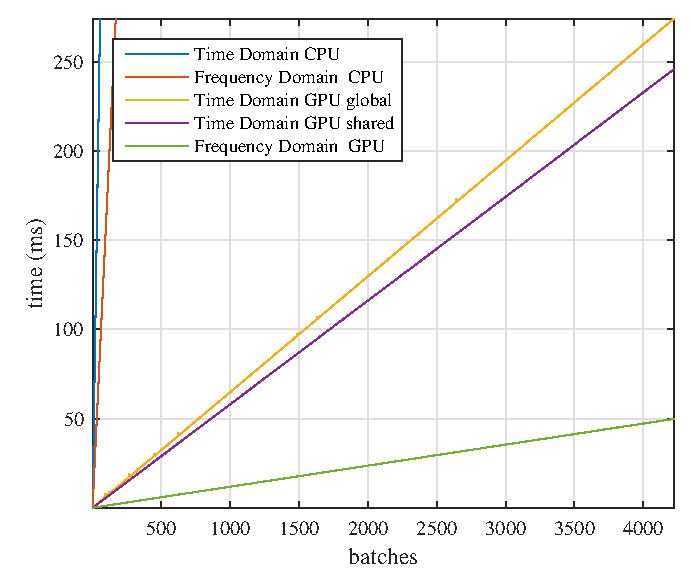
\includegraphics[width=5in]{figures/gpu_intro/CPUvsGPU_varyBatches_186taps_12672signal.eps}
	\caption{Comparison of a batched complex convolution on a CPU and GPU. The number of batches is variable while the signal and filter length is set to $12672$ and $186$.}
	\label{fig:CPUvsGPU_varyBatches_186taps_12672signal}
\end{figure}

Now that the GPU and CPU execution time is not being compared, Table \ref{tab:BatchedGPUtimingTable} shows execution times include only GPU kernels and exclude memory transfers.
Figure \ref{fig:CPUvsGPU_varyBatches_186taps_12672signal_timePerBatch} compares GPU convolution using batch processing execution time per batch as the number of packets increases.
The figure shows execution time per batch decreases as the number of packets increases but stops improving after 70 packets.
\begin{figure}
	\centering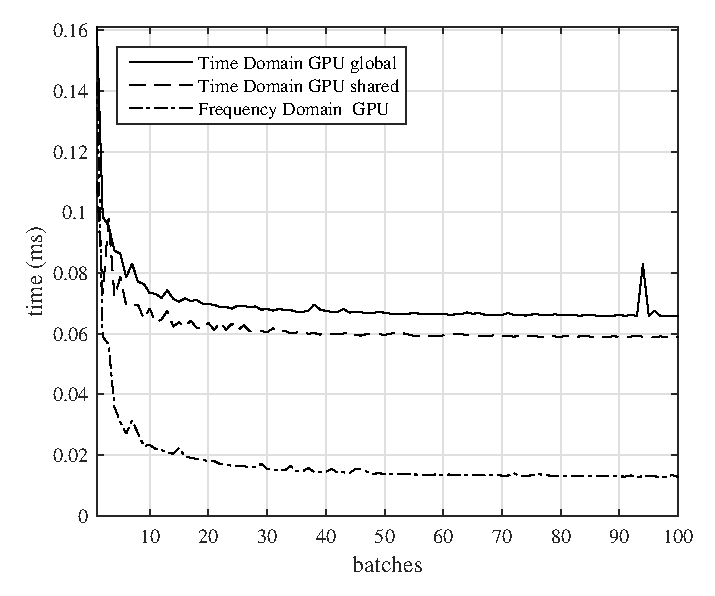
\includegraphics[width=5in]{figures/gpu_intro/CPUvsGPU_varyBatches_186taps_12672signal_timePerBatch.eps}
	\caption{Comparison on execution time per batch for complex convolution. The number of batches is variable while the signal and filter length is set to $12672$ and $186$.}
	\label{fig:CPUvsGPU_varyBatches_186taps_12672signal_timePerBatch}
\end{figure}


Figures \ref{fig:CPUvsGPU_3104batch_186taps_varySignal} through \ref{fig:CPUvsGPU_3104batch_12672signal_varyFilter} 
compare execution time of the three GPU convolution implementations by fixing the filter length with variable signal length or visa versa.
Tables \ref{tab:Batched_CPUvsGPUtable_12672_186} and \ref{tab:Batched_CPUvsGPUtable_12672_21} 
show the execution times for the signal length and filter lengths of the PAQ system when performing convolution using batch processing.
Frequency-domain convolution using batch processing is fastest for $186$ tap filters while 
time-domain convolution using batch processing and shared memory is fastest for $23$ tap filters.
\begin{figure}
	\centering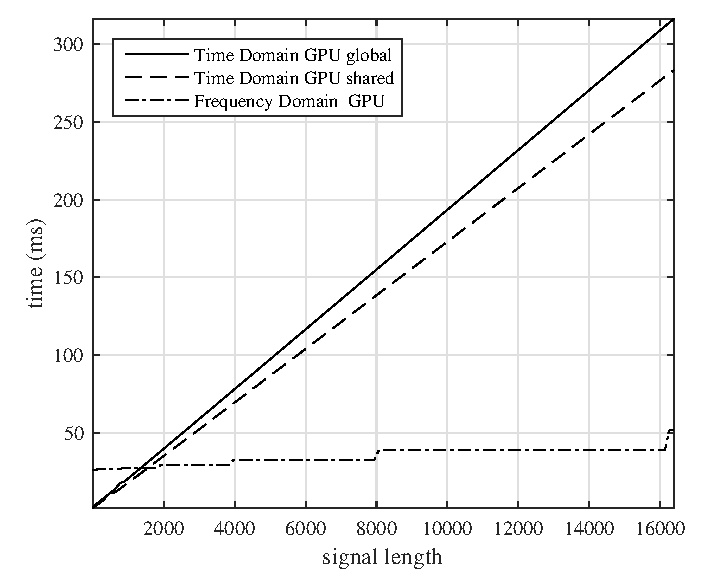
\includegraphics[width=5in]{figures/gpu_intro/CPUvsGPU_3104batch_186taps_varySignal.eps}
	\caption{Comparison of complex convolution using batch processing on a GPU. The signal length is variable and the filter is fixed at $186$ taps.}
	\label{fig:CPUvsGPU_3104batch_186taps_varySignal}
\end{figure}
\begin{figure}
	\centering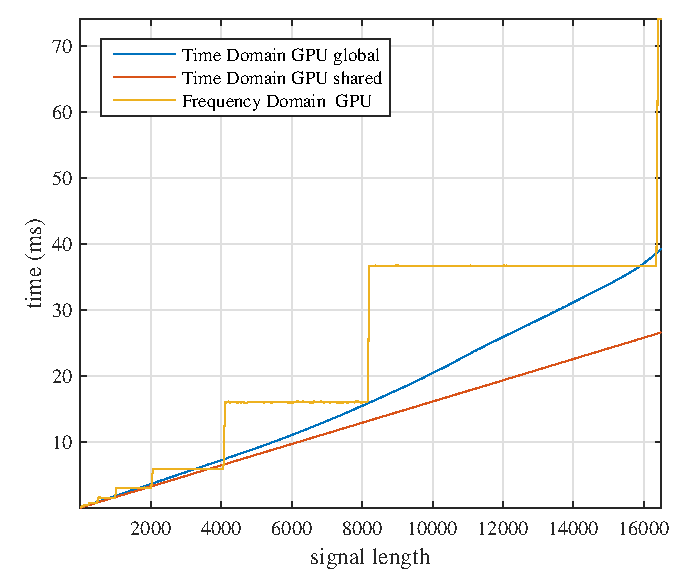
\includegraphics[width=5in]{figures/gpu_intro/CPUvsGPU_3104batch_21taps_varySignal.eps}
	\caption{Comparison of complex convolution using batch processing on a GPU. The signal length is variable and the filter is fixed at $23$ taps.}
	\label{fig:CPUvsGPU_3104batch_21taps_varySignal}
\end{figure}
\begin{figure}
	\centering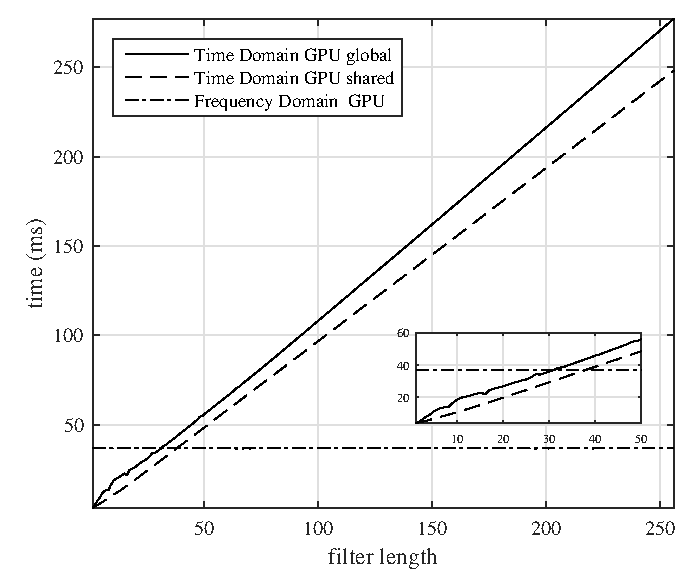
\includegraphics[width=5in]{figures/gpu_intro/CPUvsGPU_3104batch_12672signal_varyFilter.eps}
	\caption{Comparison of complex convolution using batch processing on a GPU. The filter length is variable and the signal length is set to $12672$ samples.}
	\label{fig:CPUvsGPU_3104batch_12672signal_varyFilter}
\end{figure}
\begin{table}
\caption{Convolution using batch processing execution times with for a $12672$ sample signal and $186$ tap filter on a Tesla K40c GPU.}
\begin{center}
\begin{tabular}{lll}
	\toprule
	Algorithm 				& Function or Library		& Execution Time (ms) \\ \midrule
	GPU time domain global 	& ConvGPU 					& 201.29		\\
	GPU time domain shared 	& ConvGPUshared 			& 180.272		\\
	GPU frequency domain 	& cuFFT						& 36.798 		\\ 
	\bottomrule
\end{tabular}
\end{center}
\label{tab:Batched_CPUvsGPUtable_12672_186}
\end{table}
\begin{table}
\caption{Convolution using batch processing execution times with for a $12672$ sample signal and $23$ tap filter on a Tesla K40c GPU.}
\begin{center}
\begin{tabular}{lll}
	\toprule
	Algorithm 				& Function or Library		& Execution Time (ms) \\ \midrule
	GPU time domain global 	& ConvGPU 					& 27.642		\\
	GPU time domain shared 	& ConvGPUshared 			& 20.4287		\\
	GPU frequency domain 	& cuFFT						& 36.7604		\\ 
	\bottomrule
\end{tabular}
\end{center}
\label{tab:Batched_CPUvsGPUtable_12672_21}
\end{table}

Until now, convolving one signal with only one filter has been considered.
Figure \ref{fig:thisThesisBlock} showed the received signal is filtered by two cascaded filters: 
an equalizer filter and a detection filter.
The block diagrams in Figure \ref{fig:freq_time_block_cascade} show the steps required for cascading time-domain and frequency-domain convolution.

Comparing the block diagrams in Figures \ref{fig:freq_time_block_cascade} and \ref{fig:freq_time_block}, cascading two filters in the frequency domain only requires an extra FFT and point-by-point complex multiplication while 
cascading filters in the time domain requires two time-domain convolutions.
The first time-domain convolution produces a composite filter from the convolution of the $186$ sample equalizer filter with the $23$ tap detection filter.
The second time-domain convolution applies the composite $208 = 186 + 23 - 1$ tap filter to a $12672$ sample signal.
Table \ref{tab:Batched_CPUvsGPUtable_12672_21_186} shows the execution times for the signal length and filter lengths of the PAQ system when performing cascaded convolution using batch processing.
Cascaded-convolution using batch processing in the frequency domain is fastest.
\begin{figure}
	\centering\includegraphics[width=10.28in/100*55]{figures/gpu_convolution/CascadeConvBlock.pdf}
	\caption{Block diagrams showing showing cascaded time-domain convolution and frequency-domain convolution.}
	\label{fig:freq_time_block_cascade}
\end{figure}
\begin{table}
\caption{Batched convolution execution times with for a $12672$ sample signal and cascaded $23$ and $186$ tap filter on a Tesla K40c GPU.}
\begin{center}
\begin{tabular}{lll}
	\toprule
	Algorithm 				& Function or Library		& Execution Time (ms) \\ \midrule
	GPU time domain global 	& ConvGPU 					& 223.307		\\
	GPU time domain shared 	& ConvGPUshared 			& 200.018		\\
	GPU frequency domain 	& cuFFT						& 39.0769		\\ 
	\bottomrule
\end{tabular}
\end{center}
\label{tab:Batched_CPUvsGPUtable_12672_21_186}
\end{table}



\singlespacing
\clearpage
\begin{lstlisting}[style=myCUDAstyle,language=C++,caption={CUDA code to performing complex convolution five different ways: time domain CPU, frequency domain CPU time domain GPU, time domain GPU using shared memory and frequency domain GPU.},label={code:convFun}]
#include <iostream>
#include <stdlib.h>
#include <math.h>
#include <cufft.h>
#include <fstream>
#include <string>
#include <fftw3.h>
using namespace std;


void ConvCPU(cufftComplex* y,cufftComplex* x,cufftComplex* h,int Lx,int Lh){
	for(int yIdx = 0; yIdx < Lx+Lh-1; yIdx++){
		cufftComplex temp;
		temp.x = 0;
		temp.y = 0;
		for(int hIdx = 0; hIdx < Lh; hIdx++){
			int xAccessIdx = yIdx-hIdx;
			if(xAccessIdx>=0 && xAccessIdx<Lx){
				// temp += x[xAccessIdx]*h[hIdx];
				float A = x[xAccessIdx].x;
				float B = x[xAccessIdx].y;
				float C = h[hIdx].x;
				float D = h[hIdx].y;
				cufftComplex result;
				result.x = A*C-B*D;
				result.y = A*D+B*C;
				temp.x += result.x;
				temp.y += result.y;
			}
		}
		y[yIdx] = temp;
	}

}

__global__ void ConvGPU(cufftComplex* y,cufftComplex* x,cufftComplex* h,int Lx,int Lh){
	int yIdx = blockIdx.x*blockDim.x + threadIdx.x;

	int lastThread = Lx+Lh-1;

	// don't access elements out of bounds
	if(yIdx >= lastThread)
		return;

	cufftComplex temp;
	temp.x = 0;
	temp.y = 0;
	for(int hIdx = 0; hIdx < Lh; hIdx++){
		int xAccessIdx = yIdx-hIdx;
		if(xAccessIdx>=0 && xAccessIdx<Lx){
			// temp += x[xAccessIdx]*h[hIdx];
			float A = x[xAccessIdx].x;
			float B = x[xAccessIdx].y;
			float C = h[hIdx].x;
			float D = h[hIdx].y;
			cufftComplex result;
			result.x = A*C-B*D;
			result.y = A*D+B*C;
			temp.x += result.x;
			temp.y += result.y;
		}
	}
	y[yIdx] = temp;
}


__global__ void ConvGPUshared(cufftComplex* y,cufftComplex* x,cufftComplex* h,int Lx,int Lh){
	int yIdx = blockIdx.x*blockDim.x + threadIdx.x;

	int lastThread = Lx+Lh-1;

	extern __shared__ cufftComplex h_shared[];
	if(threadIdx.x < Lh){
		h_shared[threadIdx.x] = h[threadIdx.x];
	}
	__syncthreads();

	// don't access elements out of bounds
	if(yIdx >= lastThread)
		return;

	cufftComplex temp;
	temp.x = 0;
	temp.y = 0;
	for(int hIdx = 0; hIdx < Lh; hIdx++){
		int xAccessIdx = yIdx-hIdx;
		if(xAccessIdx>=0 && xAccessIdx<Lx){
			// temp += x[xAccessIdx]*h[hIdx];
			float A = x[xAccessIdx].x;
			float B = x[xAccessIdx].y;
			float C = h_shared[hIdx].x;
			float D = h_shared[hIdx].y;
			cufftComplex result;
			result.x = A*C-B*D;
			result.y = A*D+B*C;
			temp.x += result.x;
			temp.y += result.y;
		}
	}
	y[yIdx] = temp;
}

__global__ void PointToPointMultiply(cufftComplex* v0, cufftComplex* v1, int lastThread){
	int i = blockIdx.x*blockDim.x + threadIdx.x;

	// don't access elements out of bounds
	if(i >= lastThread)
		return;
	float A = v0[i].x;
	float B = v0[i].y;
	float C = v1[i].x;
	float D = v1[i].y;

	// (A+jB)(C+jD) = (AC-BD) + j(AD+BC)
	cufftComplex result;
	result.x = A*C-B*D;
	result.y = A*D+B*C;

	v0[i] = result;
}

__global__ void ScalarMultiply(cufftComplex* vec0, float scalar, int lastThread){
	int i = blockIdx.x*blockDim.x + threadIdx.x;

	// Don't access elements out of bounds
	if(i >= lastThread)
		return;
	cufftComplex scalarMult;
	scalarMult.x = vec0[i].x*scalar;
	scalarMult.y = vec0[i].y*scalar;
	vec0[i] = scalarMult;
}

int main(){
	int N = 1000;
	int L = 186;
	int C = N + L - 1;
	int M = pow(2, ceil(log(C)/log(2)));

	cufftComplex *mySignal1;
	cufftComplex *mySignal2;
	cufftComplex *mySignal2_fft;

	cufftComplex *myFilter1;
	cufftComplex *myFilter2;
	cufftComplex *myFilter2_fft;

	cufftComplex *myConv1;
	cufftComplex *myConv2;
	cufftComplex *myConv2_timeReversed;
	cufftComplex *myConv3;
	cufftComplex *myConv4;
	cufftComplex *myConv5;

	mySignal1      		= (cufftComplex*)malloc(N*sizeof(cufftComplex));
	mySignal2      		= (cufftComplex*)malloc(M*sizeof(cufftComplex));
	mySignal2_fft  		= (cufftComplex*)malloc(M*sizeof(cufftComplex));

	myFilter1      		= (cufftComplex*)malloc(L*sizeof(cufftComplex));
	myFilter2      		= (cufftComplex*)malloc(M*sizeof(cufftComplex));
	myFilter2_fft  		= (cufftComplex*)malloc(M*sizeof(cufftComplex));

	myConv1        		= (cufftComplex*)malloc(C*sizeof(cufftComplex));
	myConv2        		= (cufftComplex*)malloc(M*sizeof(cufftComplex));
	myConv2_timeReversed= (cufftComplex*)malloc(M*sizeof(cufftComplex));
	myConv3        		= (cufftComplex*)malloc(C*sizeof(cufftComplex));
	myConv4        		= (cufftComplex*)malloc(C*sizeof(cufftComplex));
	myConv5        		= (cufftComplex*)malloc(M*sizeof(cufftComplex));

	srand(time(0));
	for(int i = 0; i < N; i++){
		mySignal1[i].x = rand()%100-50;
		mySignal1[i].y = rand()%100-50;
	}

	for(int i = 0; i < L; i++){
		myFilter1[i].x = rand()%100-50;
		myFilter1[i].y = rand()%100-50;
	}

	cufftComplex *dev_mySignal3;
	cufftComplex *dev_mySignal4;
	cufftComplex *dev_mySignal5;

	cufftComplex *dev_myFilter3;
	cufftComplex *dev_myFilter4;
	cufftComplex *dev_myFilter5;

	cufftComplex *dev_myConv3;
	cufftComplex *dev_myConv4;
	cufftComplex *dev_myConv5;

	cudaMalloc(&dev_mySignal3, N*sizeof(cufftComplex));
	cudaMalloc(&dev_mySignal4, N*sizeof(cufftComplex));
	cudaMalloc(&dev_mySignal5, M*sizeof(cufftComplex));

	cudaMalloc(&dev_myFilter3, L*sizeof(cufftComplex));
	cudaMalloc(&dev_myFilter4, L*sizeof(cufftComplex));
	cudaMalloc(&dev_myFilter5, M*sizeof(cufftComplex));

	cudaMalloc(&dev_myConv3,   C*sizeof(cufftComplex));
	cudaMalloc(&dev_myConv4,   C*sizeof(cufftComplex));
	cudaMalloc(&dev_myConv5,   M*sizeof(cufftComplex));


	/**
	 * Time-domain Convolution CPU
	 */
	ConvCPU(myConv1,mySignal1,myFilter1,N,L);

	/**
	 * Frequency Domain Convolution CPU
	 */
	fftwf_plan forwardPlanSignal = fftwf_plan_dft_1d(M, (fftwf_complex*)mySignal2,    (fftwf_complex*)mySignal2_fft, 	   FFTW_FORWARD, FFTW_MEASURE);
	fftwf_plan forwardPlanFilter = fftwf_plan_dft_1d(M, (fftwf_complex*)myFilter2, 	 (fftwf_complex*)myFilter2_fft, 	   FFTW_FORWARD, FFTW_MEASURE);
	fftwf_plan backwardPlanConv  = fftwf_plan_dft_1d(M, (fftwf_complex*)mySignal2_fft,(fftwf_complex*)myConv2_timeReversed, FFTW_FORWARD, FFTW_MEASURE);

	cufftComplex zero; zero.x = 0; zero.y = 0;
	for(int i = 0; i < M; i++){
		if(i<N)
			mySignal2[i] = mySignal1[i];
		else
			mySignal2[i] = zero;

		if(i<L)
			myFilter2[i] = myFilter1[i];
		else
			myFilter2[i] = zero;
	}

	fftwf_execute(forwardPlanSignal);
	fftwf_execute(forwardPlanFilter);

	for (int i = 0; i < M; i++){
		// mySignal2_fft = mySignal2_fft*myFilter2_fft;
		float A = mySignal2_fft[i].x;
		float B = mySignal2_fft[i].y;
		float C = myFilter2_fft[i].x;
		float D = myFilter2_fft[i].y;
		cufftComplex result;
		result.x = A*C-B*D;
		result.y = A*D+B*C;
		mySignal2_fft[i] = result;
	}

	fftwf_execute(backwardPlanConv);

	// myConv2 from fftwf must be time reversed and scaled
	// to match Matlab, myConv1, myConv3, myConv4 and myConv5
	cufftComplex result;
	for (int i = 0; i < M; i++){
		result.x = myConv2_timeReversed[M-i].x/M;
		result.y = myConv2_timeReversed[M-i].y/M;
		myConv2[i] = result;
	}
	result.x = myConv2_timeReversed[0].x/M;
	result.y = myConv2_timeReversed[0].y/M;
	myConv2[0] = result;

	fftwf_destroy_plan(forwardPlanSignal);
	fftwf_destroy_plan(forwardPlanFilter);
	fftwf_destroy_plan(backwardPlanConv);


	/**
	 * Time-domain Convolution GPU Using Global Memory
	 */
	cudaMemcpy(dev_mySignal3, mySignal1, sizeof(cufftComplex)*N, cudaMemcpyHostToDevice);
	cudaMemcpy(dev_myFilter3, myFilter1, sizeof(cufftComplex)*L, cudaMemcpyHostToDevice);

	int T_B = 512;
	int B = C/T_B;
	if(C % T_B > 0)
		B++;
	ConvGPU<<<B, T_B>>>(dev_myConv3, dev_mySignal3, dev_myFilter3, N, L);

	cudaMemcpy(myConv3, dev_myConv3, C*sizeof(cufftComplex), cudaMemcpyDeviceToHost);


	/**
	 * Time-domain Convolution GPU Using Shared Memory
	 */
	cudaMemcpy(dev_mySignal4, mySignal1, sizeof(cufftComplex)*N, cudaMemcpyHostToDevice);
	cudaMemcpy(dev_myFilter4, myFilter1, sizeof(cufftComplex)*L, cudaMemcpyHostToDevice);

	T_B = 512;
	B = C/T_B;
	if(C % T_B > 0)
		B++;
	ConvGPUshared<<<B, T_B,L*sizeof(cufftComplex)>>>(dev_myConv4, dev_mySignal4, dev_myFilter4, N, L);

	cudaMemcpy(myConv4, dev_myConv4, C*sizeof(cufftComplex), cudaMemcpyDeviceToHost);


	/**
	 * Frequency-domain Convolution GPU
	 */
	cufftHandle plan;
	int n[1] = {M};
	cufftPlanMany(&plan,1,n,NULL,1,1,NULL,1,1,CUFFT_C2C,1);

	cudaMemset(dev_mySignal5, 0, 	     M*sizeof(cufftComplex));
	cudaMemset(dev_myFilter5, 0, 	     M*sizeof(cufftComplex));

	cudaMemcpy(dev_mySignal5, mySignal2, M*sizeof(cufftComplex), cudaMemcpyHostToDevice);
	cudaMemcpy(dev_myFilter5, myFilter2, M*sizeof(cufftComplex), cudaMemcpyHostToDevice);

	cufftExecC2C(plan, dev_mySignal5, dev_mySignal5, CUFFT_FORWARD);
	cufftExecC2C(plan, dev_myFilter5, dev_myFilter5, CUFFT_FORWARD);

	T_B = 512;
	B = M/T_B;
	if(M % T_B > 0)
		B++;
	PointToPointMultiply<<<B, T_B>>>(dev_mySignal5, dev_myFilter5, M);

	cufftExecC2C(plan, dev_mySignal5, dev_mySignal5, CUFFT_INVERSE);

	T_B = 128;
	B = M/T_B;
	if(M % T_B > 0)
		B++;
	float scalar = 1.0/((float)M);
	ScalarMultiply<<<B, T_B>>>(dev_mySignal5, scalar, M);

	cudaMemcpy(myConv5, dev_mySignal5, M*sizeof(cufftComplex), cudaMemcpyDeviceToHost);

	cufftDestroy(plan);

	free(mySignal1);
	free(mySignal2);

	free(myFilter1);
	free(myFilter2);

	free(myConv1);
	free(myConv2);
	free(myConv2_timeReversed);
	free(myConv3);
	free(myConv4);
	free(myConv5);
	fftwf_cleanup();

	cudaFree(dev_mySignal3);
	cudaFree(dev_mySignal4);
	cudaFree(dev_mySignal5);

	cudaFree(dev_myFilter3);
	cudaFree(dev_myFilter4);
	cudaFree(dev_myFilter5);

	cudaFree(dev_myConv3);
	cudaFree(dev_myConv4);
	cudaFree(dev_myConv5);

	return 0;
}
\end{lstlisting}
\doublespacing

\singlespacing
\clearpage
\begin{lstlisting}[style=myCUDAstyle,language=C++,caption={CUDA code to perform batched complex convolution three different ways in a GPU: time domain using global memory, time domain using shared memory and frequency domain GPU.},label={code:batchedConvFun}]
#include <cufft.h>
#include <iostream>
using namespace std;

__global__ void ConvGPU(cufftComplex* y_out,cufftComplex* x_in,cufftComplex* h_in,int Lx,int Lh,int maxThreads){
	int threadNum = blockIdx.x*blockDim.x + threadIdx.x;
	int convLength = Lx+Lh-1;

	// Don't access elements out of bounds
	if(threadNum >= maxThreads)
		return;

	int batch = threadNum/convLength;
	int yIdx  = threadNum%convLength;
	cufftComplex* x = &x_in[Lx*batch];
	cufftComplex* h = &h_in[Lh*batch];
	cufftComplex* y = &y_out[convLength*batch];

	cufftComplex temp;
	temp.x = 0;
	temp.y = 0;
	for(int hIdx = 0; hIdx < Lh; hIdx++){
		int xAccessIdx = yIdx-hIdx;
		if(xAccessIdx>=0 && xAccessIdx<Lx){
			// temp += x[xAccessIdx]*h[hIdx];
			// (A+jB)(C+jD) = (AC-BD) + j(AD+BC)
			float A = x[xAccessIdx].x;
			float B = x[xAccessIdx].y;
			float C = h[hIdx].x;
			float D = h[hIdx].y;
			cufftComplex complexMult;
			complexMult.x = A*C-B*D;
			complexMult.y = A*D+B*C;

			temp.x += complexMult.x;
			temp.y += complexMult.y;
		}
	}
	y[yIdx] = temp;
}

__global__ void ConvGPUshared(cufftComplex* y_out,cufftComplex* x_in,cufftComplex* h_in,int Lx,int Lh,int maxThreads){

	int threadNum = blockIdx.x*blockDim.x + threadIdx.x;
	int convLength = Lx+Lh-1;
	// Don't access elements out of bounds
	if(threadNum >= maxThreads)
		return;

	int batch = threadNum/convLength;
	int yIdx  = threadNum%convLength;
	cufftComplex* x = &x_in[Lx*batch];
	cufftComplex* h = &h_in[Lh*batch];
	cufftComplex* y = &y_out[convLength*batch];

	extern __shared__ cufftComplex h_shared[];
	if(threadIdx.x < Lh)
		h_shared[threadIdx.x] = h[threadIdx.x];

	__syncthreads();

	cufftComplex temp;
	temp.x = 0;
	temp.y = 0;
	for(int hIdx = 0; hIdx < Lh; hIdx++){
		int xAccessIdx = yIdx-hIdx;
		if(xAccessIdx>=0 && xAccessIdx<Lx){
			// temp += x[xAccessIdx]*h[hIdx];
			// (A+jB)(C+jD) = (AC-BD) + j(AD+BC)
			float A = x[xAccessIdx].x;
			float B = x[xAccessIdx].y;
			float C = h_shared[hIdx].x;
			float D = h_shared[hIdx].y;
			cufftComplex complexMult;
			complexMult.x = A*C-B*D;
			complexMult.y = A*D+B*C;

			temp.x += complexMult.x;
			temp.y += complexMult.y;
		}
	}
	y[yIdx] = temp;
}

__global__ void PointToPointMultiply(cufftComplex* vec0, cufftComplex* vec1, int maxThreads){
	int i = blockIdx.x*blockDim.x + threadIdx.x;
	// Don't access elements out of bounds
	if(i >= maxThreads)
		return;
	// vec0[i] = vec0[i]*vec1[i];
	// (A+jB)(C+jD) = (AC-BD) + j(AD+BC)
	float A = vec0[i].x;
	float B = vec0[i].y;
	float C = vec1[i].x;
	float D = vec1[i].y;
	cufftComplex complexMult;
	complexMult.x = A*C-B*D;
	complexMult.y = A*D+B*C;
	vec0[i] = complexMult;
}

__global__ void ScalarMultiply(cufftComplex* vec0, float scalar, int lastThread){
	int i = blockIdx.x*blockDim.x + threadIdx.x;
	// Don't access elements out of bounds
	if(i >= lastThread)
		return;
	cufftComplex scalarMult;
	scalarMult.x = vec0[i].x*scalar;
	scalarMult.y = vec0[i].y*scalar;
	vec0[i] = scalarMult;
}

int main(){
	int numBatches = 3104;
	int N = 12672;
	int L = 186;
	int C = N + L - 1;
	int M = pow(2, ceil(log(C)/log(2)));
	int maxThreads;
	int T_B;
	int B;

	cufftHandle plan;
	int n[1] = {M};
	cufftPlanMany(&plan,1,n,NULL,1,1,NULL,1,1,CUFFT_C2C,numBatches);

	// Allocate memory on host
	cufftComplex *mySignal1;
	cufftComplex *mySignal1_pad;
	cufftComplex *myFilter1;
	cufftComplex *myFilter1_pad;
	cufftComplex *myConv1;
	cufftComplex *myConv2;
	cufftComplex *myConv3;
	mySignal1      = (cufftComplex*) malloc(N*numBatches*sizeof(cufftComplex));
	mySignal1_pad  = (cufftComplex*) malloc(M*numBatches*sizeof(cufftComplex));
	myFilter1      = (cufftComplex*) malloc(L*numBatches*sizeof(cufftComplex));
	myFilter1_pad  = (cufftComplex*) malloc(M*numBatches*sizeof(cufftComplex));
	myConv1        = (cufftComplex*) malloc(C*numBatches*sizeof(cufftComplex));
	myConv2        = (cufftComplex*) malloc(C*numBatches*sizeof(cufftComplex));
	myConv3        = (cufftComplex*) malloc(M*numBatches*sizeof(cufftComplex));

	srand(time(0));
	for(int i = 0; i < N; i++){
		mySignal1[i].x = rand()%100-50;
		mySignal1[i].y = rand()%100-50;
	}

	for(int i = 0; i < L; i++){
		myFilter1[i].x = rand()%100-50;
		myFilter1[i].y = rand()%100-50;
	}

	cufftComplex zero;
	zero.x = 0;
	zero.y = 0;
	for(int i = 0; i<M*numBatches; i++){
		mySignal1_pad[i] = zero;
		myFilter1_pad[i] = zero;
	}
	for(int batch=0; batch < numBatches; batch++){
		for(int i = 0; i < N; i++){
			mySignal1[batch*N+i] = mySignal1[i];
			mySignal1_pad[batch*M+i] = mySignal1[i];
		}
		for(int i = 0; i < L; i++){
			myFilter1[batch*L+i] = myFilter1[i];
			myFilter1_pad[batch*M+i] = myFilter1[i];
		}
	}

	// Allocate memory on device
	cufftComplex *dev_mySignal1;
	cufftComplex *dev_mySignal2;
	cufftComplex *dev_mySignal3;
	cufftComplex *dev_myFilter1;
	cufftComplex *dev_myFilter2;
	cufftComplex *dev_myFilter3;
	cufftComplex *dev_myConv1;
	cufftComplex *dev_myConv2;
	cufftComplex *dev_myConv3;
	cudaMalloc(&dev_mySignal1, N*numBatches*sizeof(cufftComplex));
	cudaMalloc(&dev_mySignal2, N*numBatches*sizeof(cufftComplex));
	cudaMalloc(&dev_mySignal3, M*numBatches*sizeof(cufftComplex));
	cudaMalloc(&dev_myFilter1, L*numBatches*sizeof(cufftComplex));
	cudaMalloc(&dev_myFilter2, L*numBatches*sizeof(cufftComplex));
	cudaMalloc(&dev_myFilter3, M*numBatches*sizeof(cufftComplex));
	cudaMalloc(&dev_myConv1,   C*numBatches*sizeof(cufftComplex));
	cudaMalloc(&dev_myConv2,   C*numBatches*sizeof(cufftComplex));
	cudaMalloc(&dev_myConv3,   M*numBatches*sizeof(cufftComplex));

	/**
	 * Time-domain Convolution GPU Using Global Memory
	 */
	cudaMemcpy(dev_mySignal1, mySignal1, numBatches*sizeof(cufftComplex)*N, cudaMemcpyHostToDevice);
	cudaMemcpy(dev_myFilter1, myFilter1, numBatches*sizeof(cufftComplex)*L, cudaMemcpyHostToDevice);

	maxThreads = C*numBatches;
	T_B = 128;
	B = maxThreads/T_B;
	if(maxThreads % T_B > 0)
		B++;
	ConvGPU<<<B, T_B>>>(dev_myConv1, dev_mySignal1, dev_myFilter1, N, L, maxThreads);

	cudaMemcpy(myConv1, dev_myConv1, C*numBatches*sizeof(cufftComplex), cudaMemcpyDeviceToHost);

	/**
	 * Time-domain Convolution GPU Using Shared Memory
	 */
	cudaMemcpy(dev_mySignal2, mySignal1, numBatches*sizeof(cufftComplex)*N, cudaMemcpyHostToDevice);
	cudaMemcpy(dev_myFilter2, myFilter1, numBatches*sizeof(cufftComplex)*L, cudaMemcpyHostToDevice);

	maxThreads = C*numBatches;
	T_B = 256;
	B = maxThreads/T_B;
	if(maxThreads % T_B > 0)
		B++;
	ConvGPUshared<<<B, T_B, L*sizeof(cufftComplex)>>>(dev_myConv2, dev_mySignal2, dev_myFilter2, N, L,maxThreads);

	cudaMemcpy(myConv2, dev_myConv2, C*numBatches*sizeof(cufftComplex), cudaMemcpyDeviceToHost);

	/**
	 * Frequency-domain Convolution GPU
	 */
	cudaMemcpy(dev_mySignal3, mySignal1_pad, M*numBatches*sizeof(cufftComplex), cudaMemcpyHostToDevice);
	cudaMemcpy(dev_myFilter3, myFilter1_pad, M*numBatches*sizeof(cufftComplex), cudaMemcpyHostToDevice);

	cufftExecC2C(plan, dev_mySignal3, dev_mySignal3, CUFFT_FORWARD);
	cufftExecC2C(plan, dev_myFilter3, dev_myFilter3, CUFFT_FORWARD);

	maxThreads = M*numBatches;
	T_B = 96;
	B = maxThreads/T_B;
	if(maxThreads % T_B > 0)
		B++;
	PointToPointMultiply<<<B, T_B>>>(dev_mySignal3, dev_myFilter3, maxThreads);
	cufftExecC2C(plan, dev_mySignal3, dev_mySignal3, CUFFT_INVERSE);

	T_B = 640;
	B = maxThreads/T_B;
	if(maxThreads % T_B > 0)
		B++;
	float scalar = 1.0/((float)M);
	ScalarMultiply<<<B, T_B>>>(dev_mySignal3, scalar, maxThreads);

	cudaMemcpy(myConv3, dev_mySignal3, M*numBatches*sizeof(cufftComplex), cudaMemcpyDeviceToHost);

	cufftDestroy(plan);

	// Free vectors on CPU
	free(mySignal1);
	free(myFilter1);
	free(myConv1);
	free(myConv2);
	free(myConv3);

	// Free vectors on GPU
	cudaFree(dev_mySignal1);
	cudaFree(dev_mySignal2);
	cudaFree(dev_mySignal3);
	cudaFree(dev_myFilter1);
	cudaFree(dev_myFilter2);
	cudaFree(dev_myFilter3);
	cudaFree(dev_myConv1);
	cudaFree(dev_myConv2);
	cudaFree(dev_myConv3);

	return 0;
}
\end{lstlisting}
\doublespacing
\chapter{Equalizer GPU Implementation}
\label{chap:equalizers_in_gpus}
Each equalizer in the PAQ presents an interesting challenge from a GPU implementation perspective.
The equations for each equalizer in Section \ref{sec:equalizer_eq} were reformulated in preparation for fast and efficient GPU implementation.
This chapter is explain how the FIR equalizer filter coefficients are computed and applied.

Every equalizer filter is computed using batch processing.
In batch processing, each packet is totally independent of all other packets.
To simplify figures, every block diagram in this chapter shows how one packet is processed.
Each packet in a batch is processed exactly the same way with different data.
If a block diagram shows how to compute one equalizer filter, the block diagram is repeated $3104$ times compute a full batch of equalizer filters.

Convolution is used many times in this chapter.
Section \ref{sec:batched_convolution} showed that GPU frequency-domain batch convolution performs best for the PAQ system.
To simplify block diagrams, frequency-domain batch convolution is shown as one block.
Figures \ref{fig:Conv2} and \ref{fig:Conv3} show how frequency-domain batch convolution is represented in this chapter.
Note that the FFT of the ``numerically optimized'' detection filter $\mathbf{H}_\text{NO}$ and the SOQPSK-TG power spectrum $\mathbf{\Psi}$ are pre-computed and do not require an additional FFT block.
\begin{figure}
	\centering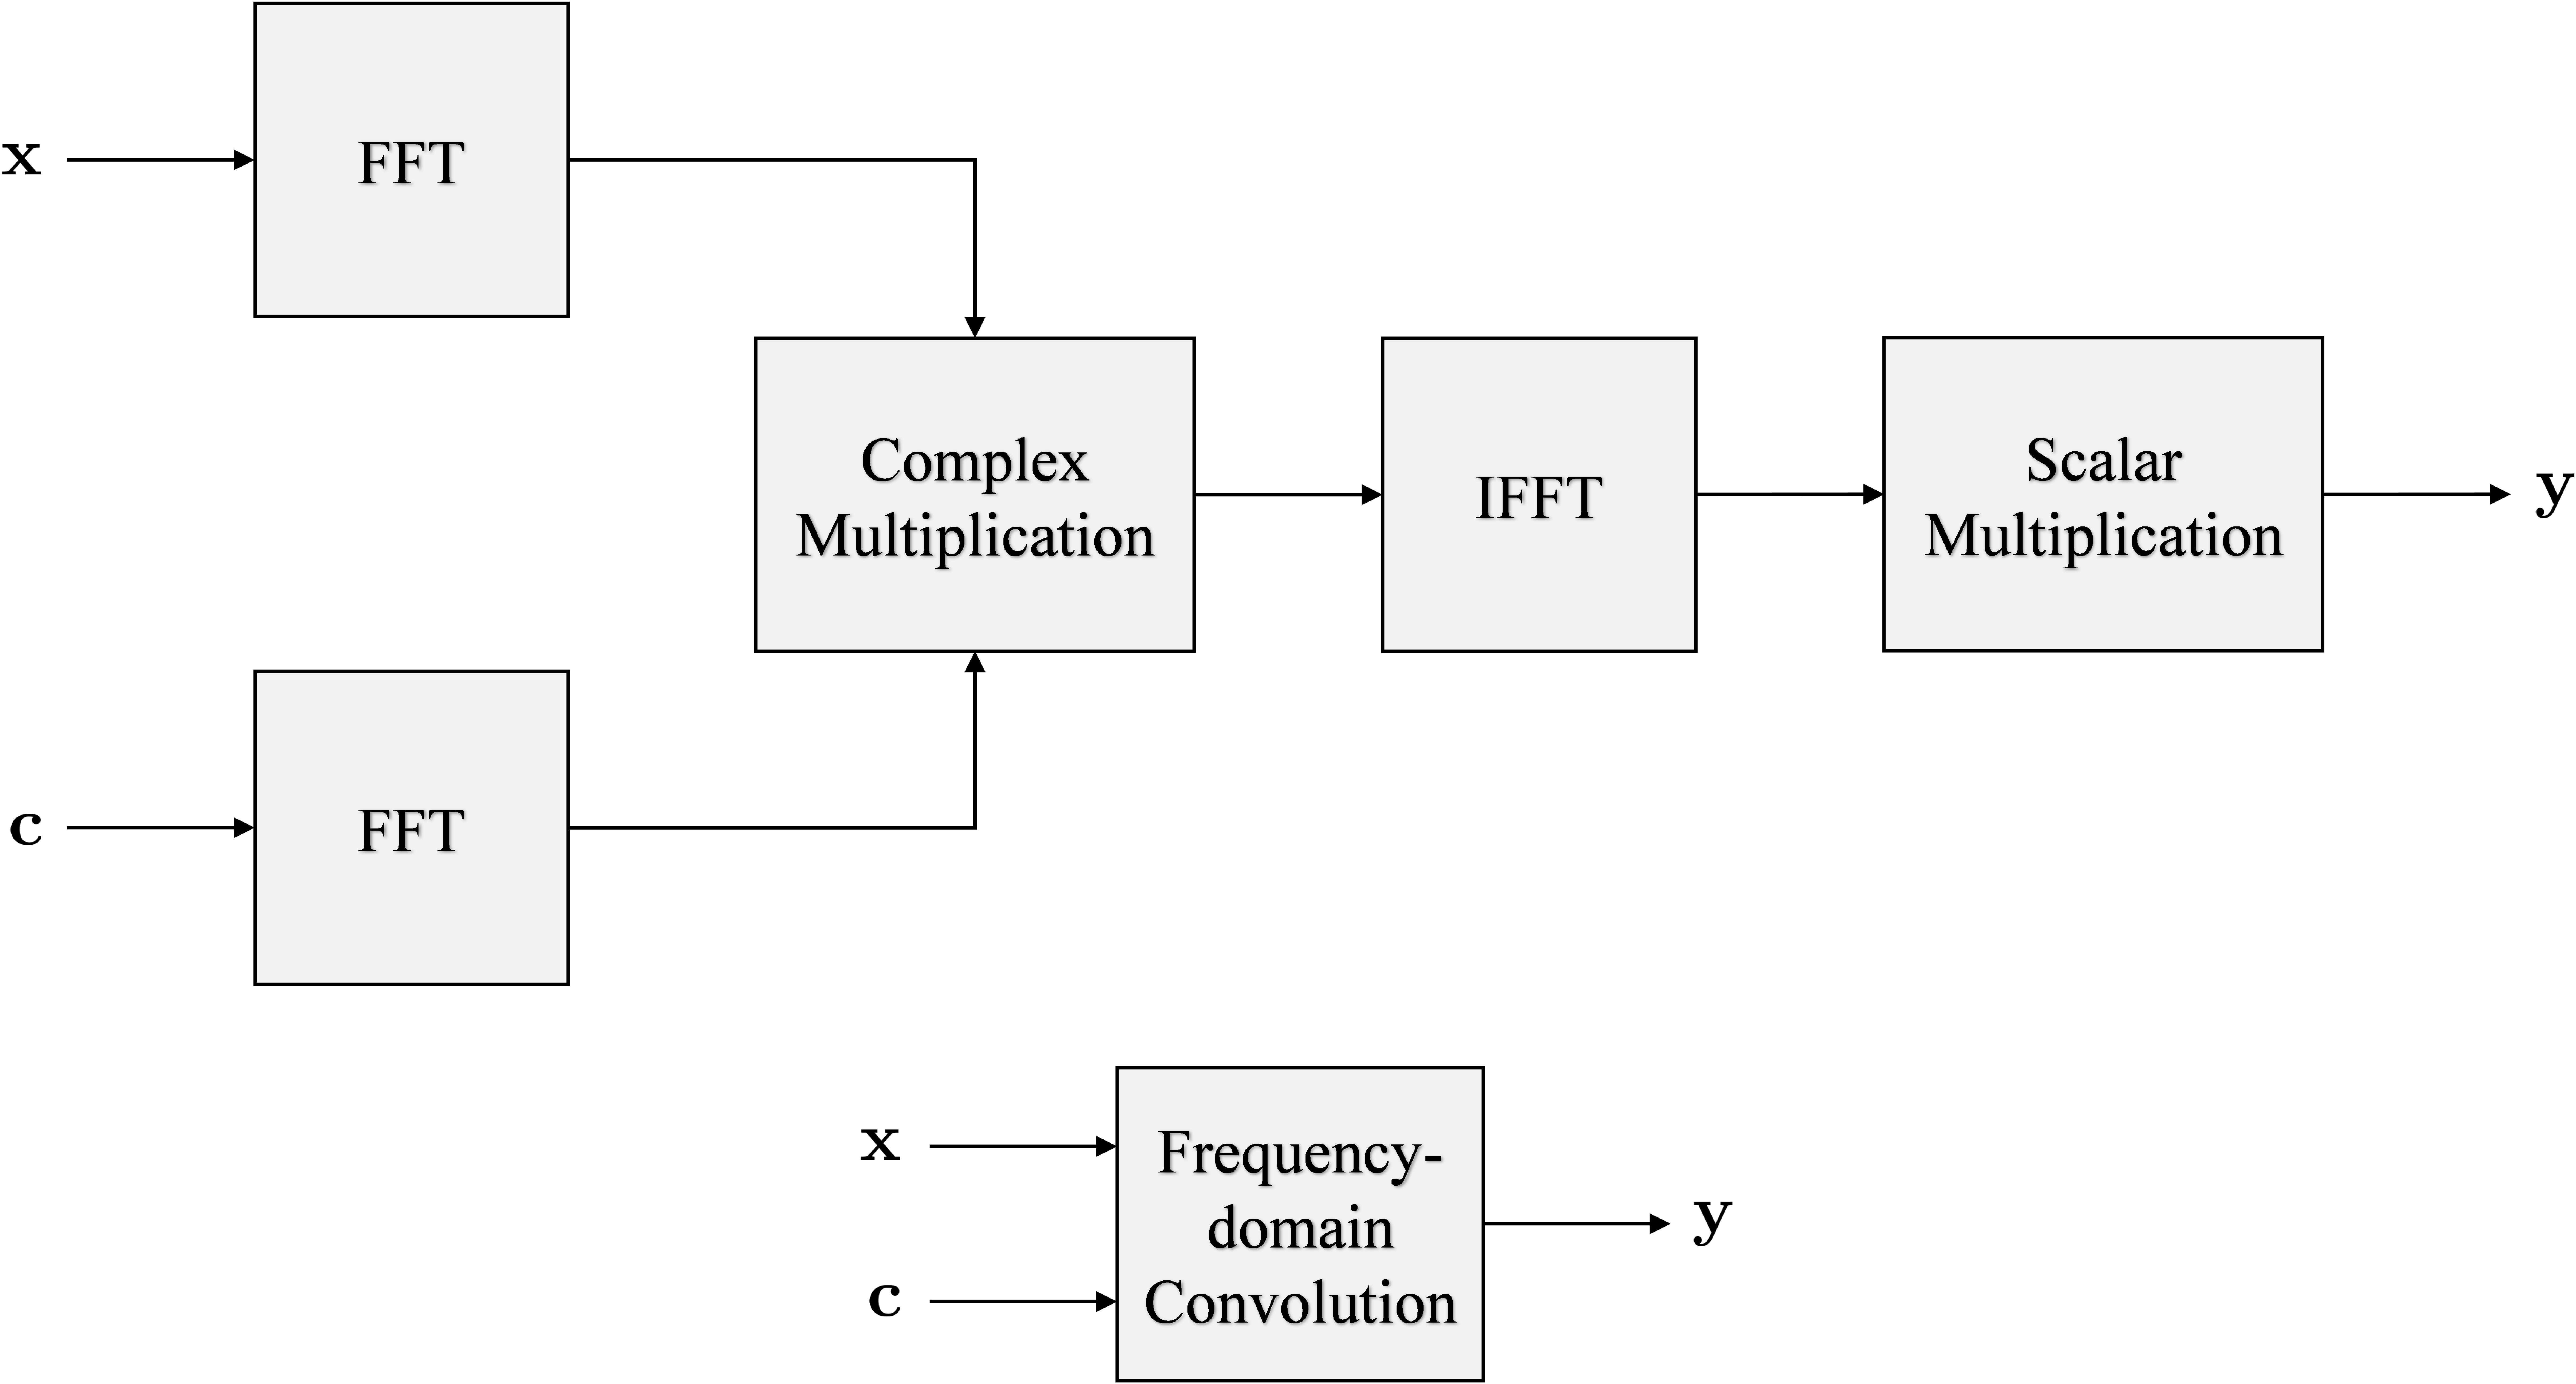
\includegraphics[width=10.28in/100*55]{figures/eq_GPUimplementation/Conv2.pdf}
	\caption{To simplify block diagrams, frequency-domain convolution is shown as one block.}
	\label{fig:Conv2}
\end{figure}
\begin{figure}
	\centering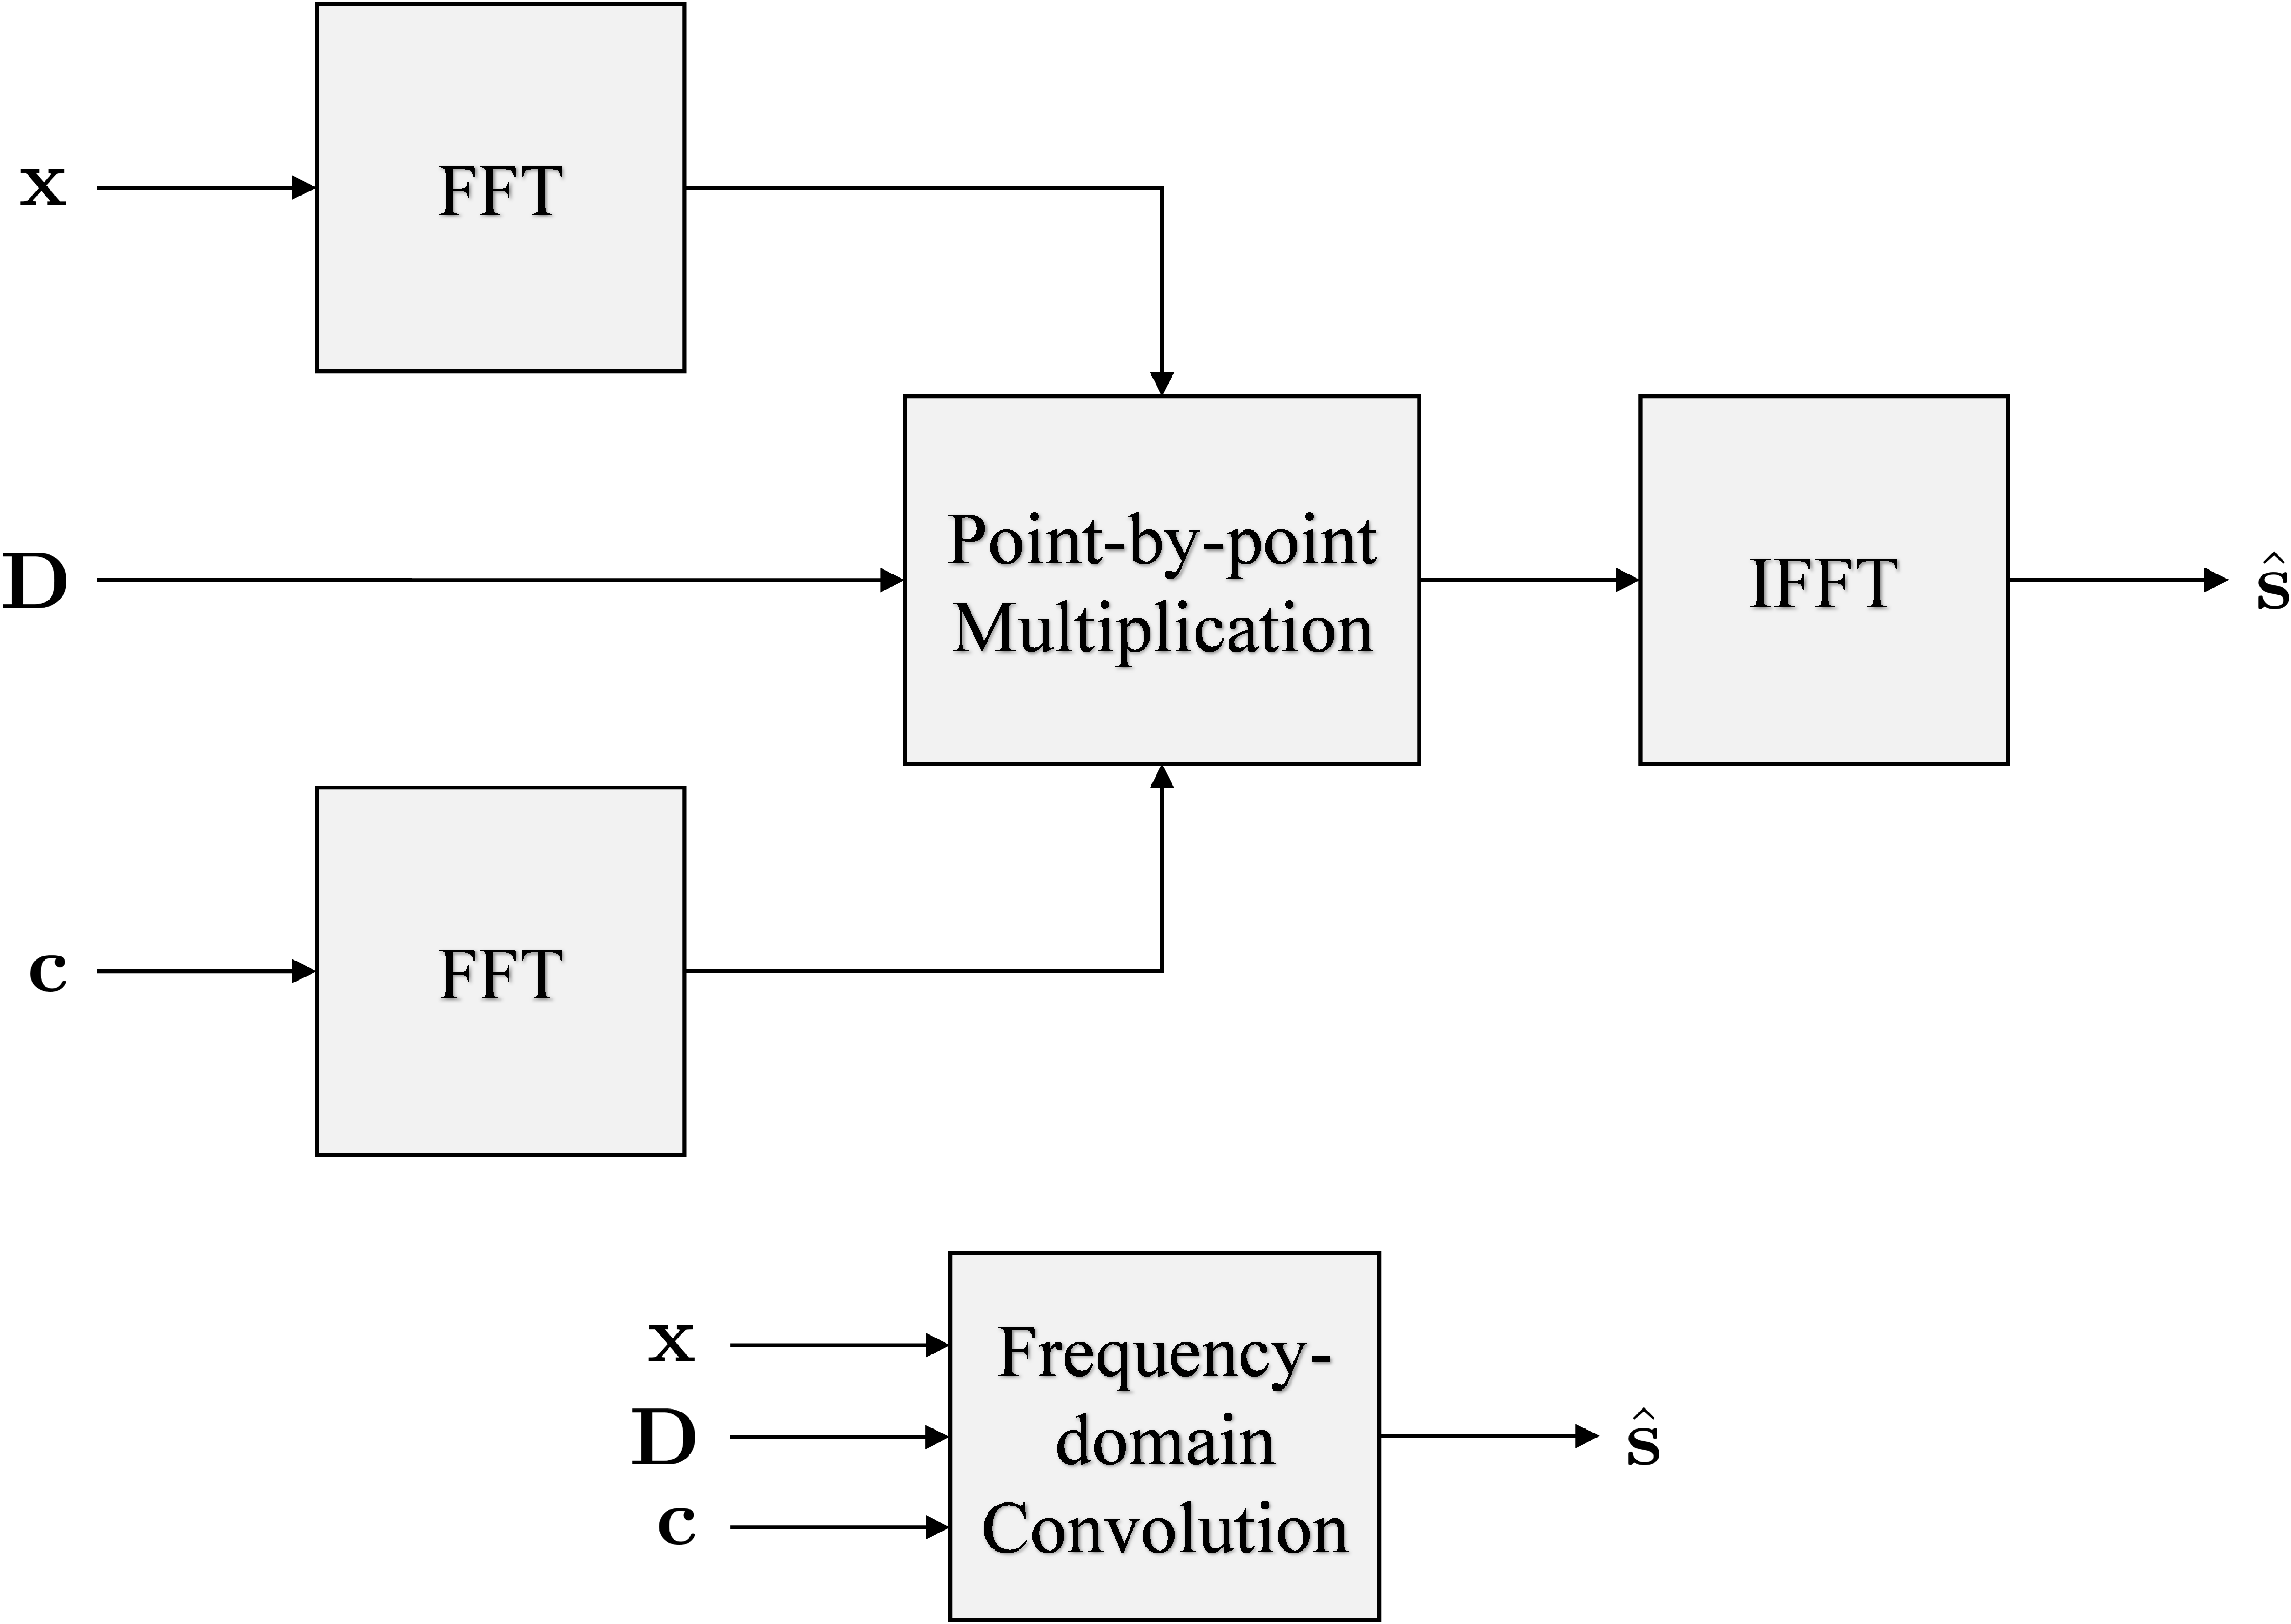
\includegraphics[width=10.28in/100*55]{figures/eq_GPUimplementation/Conv3.pdf}
	\caption{To simplify block diagrams, frequency-domain cascaded convolution is shown as one block.}
	\label{fig:Conv3}
\end{figure}

\clearpage
\section{Zero-Forcing and MMSE GPU Implementation}
The ZF and MMSE FIR equalizer filter coefficient computations have exactly the same form as shown in Equations \eqref{eq:c_ZF_solve} and \eqref{eq:c_MMSE_solve}. For reference, the equations are 
\begin{equation}
\mathbf{R}_{\hat{h}} \mathbf{c}_\text{ZF} = \hat{\mathbf{h}}_{n_0} \quad \text{or} \quad \mathbf{c}_\text{ZF} = \mathbf{R}_{\hat{h}}^{-1}\hat{\mathbf{h}}_{n_0}
\label{eq:ZF_gpuimp_solve}
\end{equation}
\begin{equation}
\mathbf{R} \mathbf{c}_\text{MMSE} = \hat{\mathbf{h}}_{n_0} \quad \text{or} \quad \mathbf{c}_\text{MMSE} = \mathbf{R}^{-1} \hat{\mathbf{h}}_{n_0}
\label{eq:MMSE_gpuimp_solve}
\end{equation}
where $\mathbf{c}_\text{ZF}$, $\mathbf{c}_\text{MMSE}$ and $\hat{\mathbf{h}}_{n_0}$ are $186\times1$ vectors and  $\mathbf{R}$ and $\mathbf{R}_{\hat{h}}$ are $186\times186$ matrices.
The only difference between ZF and MMSE is the matrix $\mathbf{R} = 
\mathbf{R}_{\hat{h}} + 2\hat{\sigma^2_w} \mathbf{I}_{L_1+L_2+1}$.

Before solving Equations \eqref{eq:ZF_gpuimp_solve} or \eqref{eq:ZF_gpuimp_solve}, $\mathbf{R}_{\hat{h}}$, $\mathbf{R}$ and $\hat{\mathbf{h}}_{n_0}$ need to be computed given $\hat{\mathbf{h}}$.
The matrices $\mathbf{R}_{\hat{h}}$ and $\mathbf{R}$ require the sample auto-correlation of the estimated channel $\mathbf{r}_{\hat{h}}$.
$\hat{\mathbf{h}}_{n_0}$ is the channel estimate time reversed and shifted.

The equalizer filters can be computed by either solving the linear system for $\mathbf{c}_\text{ZF}$ and $\mathbf{c}_\text{MMSE}$ or by computing the inverse of $\mathbf{R}$ and $\mathbf{R}_{\hat{h}}$ then performing a matrix vector multiplication.
Both techniques require $\mathcal{O}(n^3)$ operations making the computation of the ZF and MMSE equalizer filter coefficients extremely heavy.
Computing a matrix inverse or solving linear systems in GPUs is especially challenging because common algorithms are serial.
Three approaches to computing the equalizer filter coefficients was explored
\begin{itemize}
\item Levinson-Durbin recursion to solve the system of equations
\item using the cuBLAS LU decomposition library to compute the inverse and matrix vector multiplication
\item Using the cuSolver library to solve the system of equations.
\end{itemize}

Levinson-Durbin recursion avoids $\mathcal{O}(n^3)$ operations by using the Toeplitz or diagonal-constant structure of $\mathbf{R}_{\hat{h}}$ and $\mathbf{R}$ \cite[Chap. 5]{hayes:1996}.
To begin implementing Levinson-Durbin recursion, a custom GPU kernel was designed for 32-bit \textit{real} floating point data by computing $3104$ packets of ZF and MMSE equalizer filter coefficients.
Levinson-Durbin recursion showed promise by executing on real data in $500$ ms.
The algorithm was then tested on 32-bit \textit{complex} floating point data by computing $3104$ packets of  float ZF and MMSE equalizer filter coefficients.
Levinson-Durbin recursion was eliminated because execution time for complex filter coefficients was $2500$ ms.
All processing must be completed in $1907$ ms.

The next algorithm explored was computing the inverse of $\mathbf{R}_{\hat{h}}$ and $\mathbf{R}$ using the batch processing cuBLAS library. 
The cuBLAS library computes a \textit{complex} 32-bit floating point inverse using LU decompositing in $600$ ms.
cuBLAS executed faster than Levinson-Durbin recursion but $600$ ms is still $\%31$ of the total $1907$ ms processing time.

The final and fastest algorithm explored solves the linear system using the batch processing cuSolverSp library.
``cusolverSpCcsrqrsvBatched'' is the GPU function used from the cuSolverSp library.
cusolverSpCcsrqrsvBatched is a complex batch solver that leverages the sparse properties of $\mathbf{R}_{\hat{h}}$ and $\mathbf{R}$ by utilizing Compressed Row Storage (CRS) \cite{wiki:Sparse_matrix}.
The Compressed Row Storage reduces the large $186\times186$ matrices to $12544$ element CSR matrices $\mathbf{R}_{\hat{h}\text{CRS}}$ and $\mathbf{R}_{\text{CRS}}$.
Before cusolverSpCcsrqrsvBatched can be called, the CSR matrix $\mathbf{R}_{\hat{h}\text{CRS}}$ has to be built using $\mathbf{r}_{\hat{h}}$.
An example of how to use the CUDA cusolverSp library can be found \cite{CUDA_toolkit_doc}.

Figures \ref{fig:blockZF} and \ref{fig:blockMMSE} show how the ZF and MMSE equalizer filters are computed and applied to the received samples.
Note that the equalizer filters are applied in the frequency-domain with the detection filter.
\begin{figure}
	\centering\includegraphics[width=7.5in/100*55]{figures/eq_GPUimplementation/blockZF.pdf}
	\caption{Block Diagram showing how the Zero-Forcing equalizer coefficients are implemented in the GPU.}
	\label{fig:blockZF}
\end{figure}
\begin{figure}
	\centering\includegraphics[width=7.98in/100*55]{figures/eq_GPUimplementation/blockMMSE.pdf}
	\caption{Block Diagram showing how the Minimum Mean Squared Error equalizer coefficients are implemented in the GPU.}
	\label{fig:blockMMSE}
\end{figure}
Table \ref{tab:ZFMMSEtimingComparison} lists the algorithms researched and their respective execution times.
\begin{table}
\caption{Defining start and stop lines for timing comparison in Listing \ref{code:convFun}.}
\begin{center}
\begin{tabular}{lll}
	\toprule
	Algorithm 			& Data type	& Execution Time (ms)	\\ \midrule
	Levinson Recursion 	& floats 	& 500 					\\
	Levinson Recursion 	& Complex 	& 2500 					\\
	LU Decomposition 	& Complex 	& 600				 	\\
	cuSolver			& Complex	& 355.96				\\
	\bottomrule
\end{tabular}
\end{center}
\label{tab:ZFMMSEtimingComparison}
\end{table}

\clearpage
\section{Constant Modulus Algorithm GPU Implementation}
The Constant Modulus Algorithm (CMA) computes FIR equalizer filter coefficients by a steepest decent algorithm in Equation \eqref{eq:steepest}.
The more iterations a steepest decent algorithm executes, the better the CMA equalizer file will be.
The cost function gradient used in the steepest decent algorithm is $\nabla J$ shown in Equation \eqref{eq:DelJcma-midMassage}.
These equations are shown here for reference:
\begin{equation}
\mathbf{c}_\text{CMA($b+1$)} = \mathbf{c}_\text{CMA($b$)}-\mu \nabla J
\end{equation}
\begin{equation}
	\nabla J = \frac{1}{L_{pkt}} \sum_{n=0}^{L_{pkt}-1}
	z(n)  \mathbf{r}^\ast(n) \quad or \quad \nabla J(k) = \frac{1}{L_{pkt}} b(k), \quad -L_1 \leq k \leq L_2
	\label{eq:CMA_challenge}
\end{equation}
where
\begin{equation}
z(n) = 	2\left[ \vphantom{\displaystyle\sum}  y(n) y^\ast(n) - 1 \right] y(n),
\end{equation} 
\begin{align}
b(n) &= \sum^{L_{pkt}-1}_{m=0} z(m) \rho(n-m)
\end{align}
and
\begin{equation}
\rho(n) = r^\ast(n).
\end{equation}

The most computationally heavy portion of the CMA equalizer filter implementation is computing the cost function gradient $\nabla J$ in Equation \eqref{eq:CMA_challenge}.
Section \ref{sec:CMA} showed there is two approaches to computing $\nabla J$: directly or using convolution.

The direct approach didn't allow for multiple iterations because each equalizer filter coefficient required a $12672$ sample summation.
The summation in GPU kernels performs poorly because every equalizer filter coefficient accesses the full packet of received samples.
One CMA iteration took $421.317$ ms to execute computing $\nabla J$ directly also applying $\mathbf{c}_\text{CMA($b$)}$ and computing $\mathbf{c}_\text{CMA($b+1$)}$.

Using convolution to compute $\nabla J$ majorly decreased execution time for the CMA equalizer filter.
One CMA iteration took $88.774$ ms to execute computing $\nabla J$ using frequency-domain convolution also applying $\mathbf{c}_\text{CMA($b$)}$ and computing $\mathbf{c}_\text{CMA($b+1$)}$.
Note that all other frequency-domain convolution in this thesis $2^{14}$ or $16384$ points, but the convolution length $12672+12672-1$ is greater than $16384$. 
The FFTs in the computation of $\nabla J(k)$ are $2^{15}$ or $32768$ point FFTs.

Figure \ref{fig:blockCMA} shows a block diagram of how the CMA equalizer runs on the GPU.
Note that the detection filter is applied only on the last iteration.
Table \ref{tab:CMAtimingComparison} lists the comparison on computing $\nabla J(k)$ verse using convolution.
By reformulating the computation of $\nabla J$, the execution time was reduced by $4.74$ times.
The number of CMA iterations went from 2 iterations using direct implementations to 12 iterations using the convolution implementation.
\begin{figure}
	\centering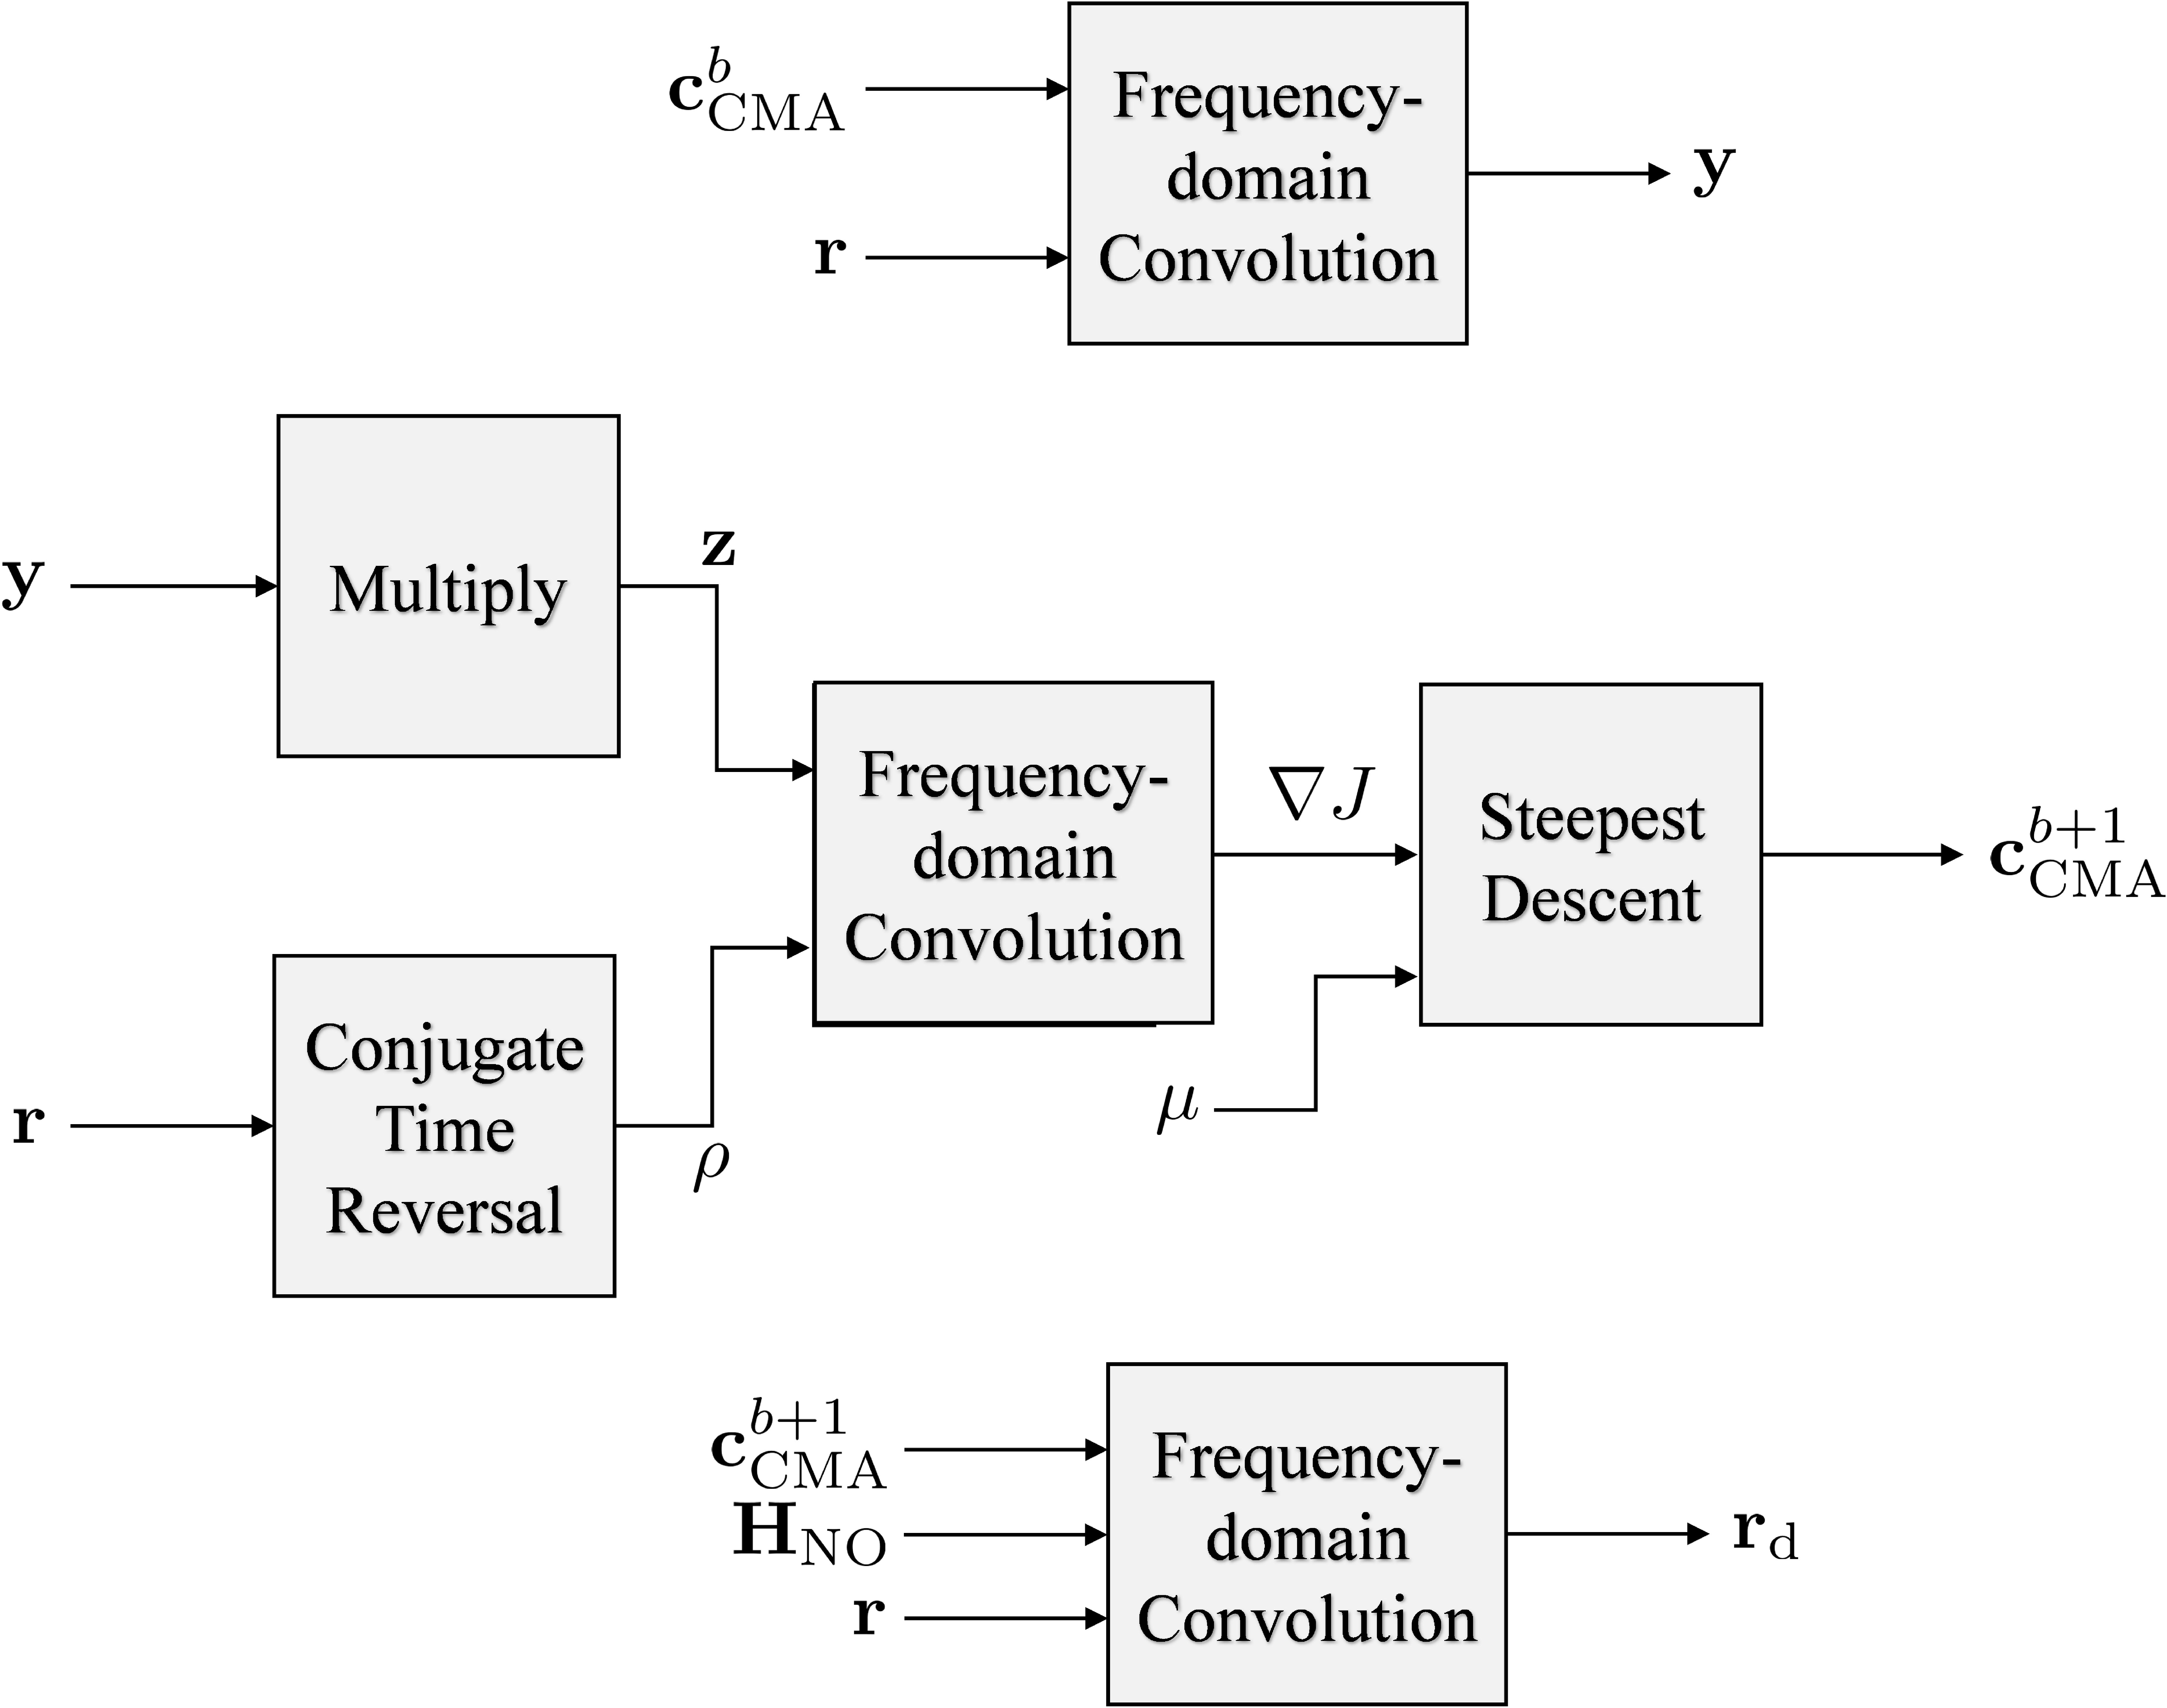
\includegraphics[width=8.34in/100*55]{figures/eq_GPUimplementation/blockCMA.pdf}
	\caption{Block Diagram showing how the CMA equalizer filter is implemented in the GPU using frequency-domain convolution twice per iteration.}
	\label{fig:blockCMA}
\end{figure}
\begin{table}
\caption{The gradient vector $\nabla J$ can be computed directly or using convolution.}
\begin{center}
\begin{tabular}{lll}
	\toprule
	CMA	Iteration Algorithm		& Execution Time (ms)	\\ \midrule
	$\nabla J$ directly 		& 421.317				\\
	$\nabla J$ using convolution & 88.774				\\
	\bottomrule
\end{tabular}
\end{center}
\label{tab:CMAtimingComparison}
\end{table}

\section{Frequency Domain Equalizer One and Two GPU Implementation}
The Frequency Domain Equalizers (FDEs) were by far the fastest and easiest to implement into GPUs.
The block diagram looks just like convolution except that complex multiplication is
\begin{equation}
R_\text{d1}(e^{j\omega_k}) = \frac{R(e^{j\omega_k}) \hat{H}^\ast(e^{j\omega_k}) H_{\text{NO}}(e^{j\omega_k})}  {|\hat{H}(e^{j\omega_k})|^2  +  \frac{1}{\hat{\sigma}^2_w}} \quad
\text{where} \;
\omega_k = \frac{2\pi}{L} \;
\text{for} \;
k=0,1,\cdots,L-1
\label{eq:FDE1_applied}
\end{equation}
or
\begin{equation}
R_\text{d2}(e^{j\omega_k}) = \frac{R(e^{j\omega_k}) \hat{H}^\ast(e^{j\omega_k}) H_{\text{NO}}(e^{j\omega_k})}  {|\hat{H}(e^{j\omega_k})|^2  +  \frac{\Psi(e^{j\omega_k})}{\hat{\sigma}^2_w}} \quad
\text{where} \;
\omega_k = \frac{2\pi}{L} \;
\text{for} \;
k=0,1,\cdots,L-1
\label{eq:FDE2_applied}
\end{equation}
where $R(e^{j\omega_k})$ and $R_\text{d}(e^{j\omega_k})$ is the FFT $\mathbf{r}$ and $\mathbf{r}_\text{d}$ 
at $\omega_k$.
Equations \eqref{eq:FDE1_applied} and \ref{eq:FDE2_applied} apply FDE1 and FDE2 from Equations \eqref{eq:FDE1} and \eqref{eq:FDE2} to the received samples and apply the detection filter.
Figures \ref{fig:blockFDE1} and \ref{fig:blockFDE2} show the block diagrams for GPU implementation.
As expected, these figures look just like the frequency-domain convolution block diagrams shown in Figures \ref{fig:Conv2} and \ref{fig:Conv3}.
Table \ref{tab:FDEtimingComparison} shows the execution times for calculating and applying FDE1 and FDE2.
\begin{table}
\caption{Execution times for calculating and applying Frequency Domain Equalizer One and Two.}
\begin{center}
\begin{tabular}{lll}
	\toprule
	Algorithm						& Execution Time (ms)	\\ \midrule
	Frequency Domain Equalizer One 	& 57.156				\\
	Frequency Domain Equalizer Two	& 58.841				\\
	\bottomrule
\end{tabular}
\end{center}
\label{tab:FDEtimingComparison}
\end{table}
\begin{figure}
	\centering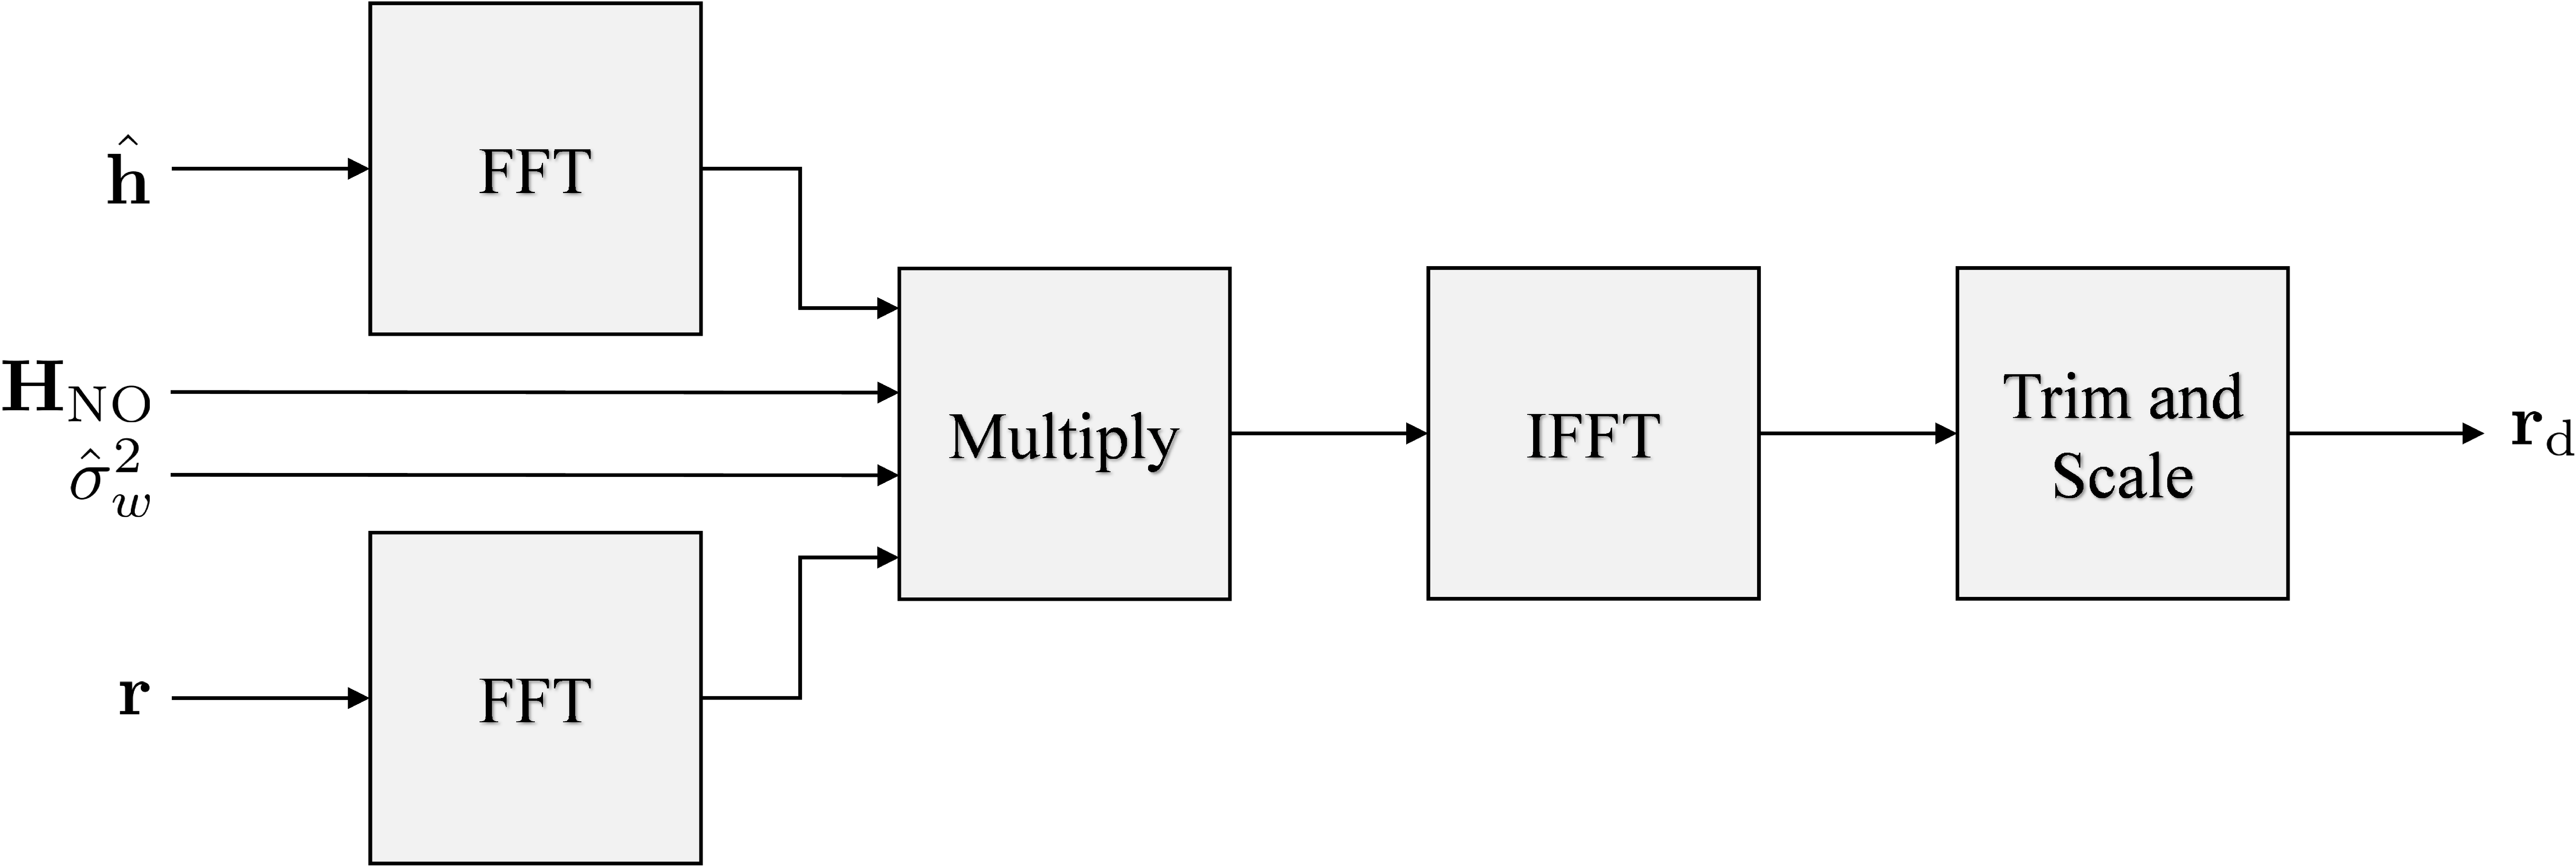
\includegraphics[width=9.73in/100*55]{figures/eq_GPUimplementation/blockFDE1.pdf}
	\caption{Diagram showing Frequency Domain Equalizer One is implemented in the frequency domain in GPUs.}
	\label{fig:blockFDE1}
\end{figure}
\begin{figure}
	\centering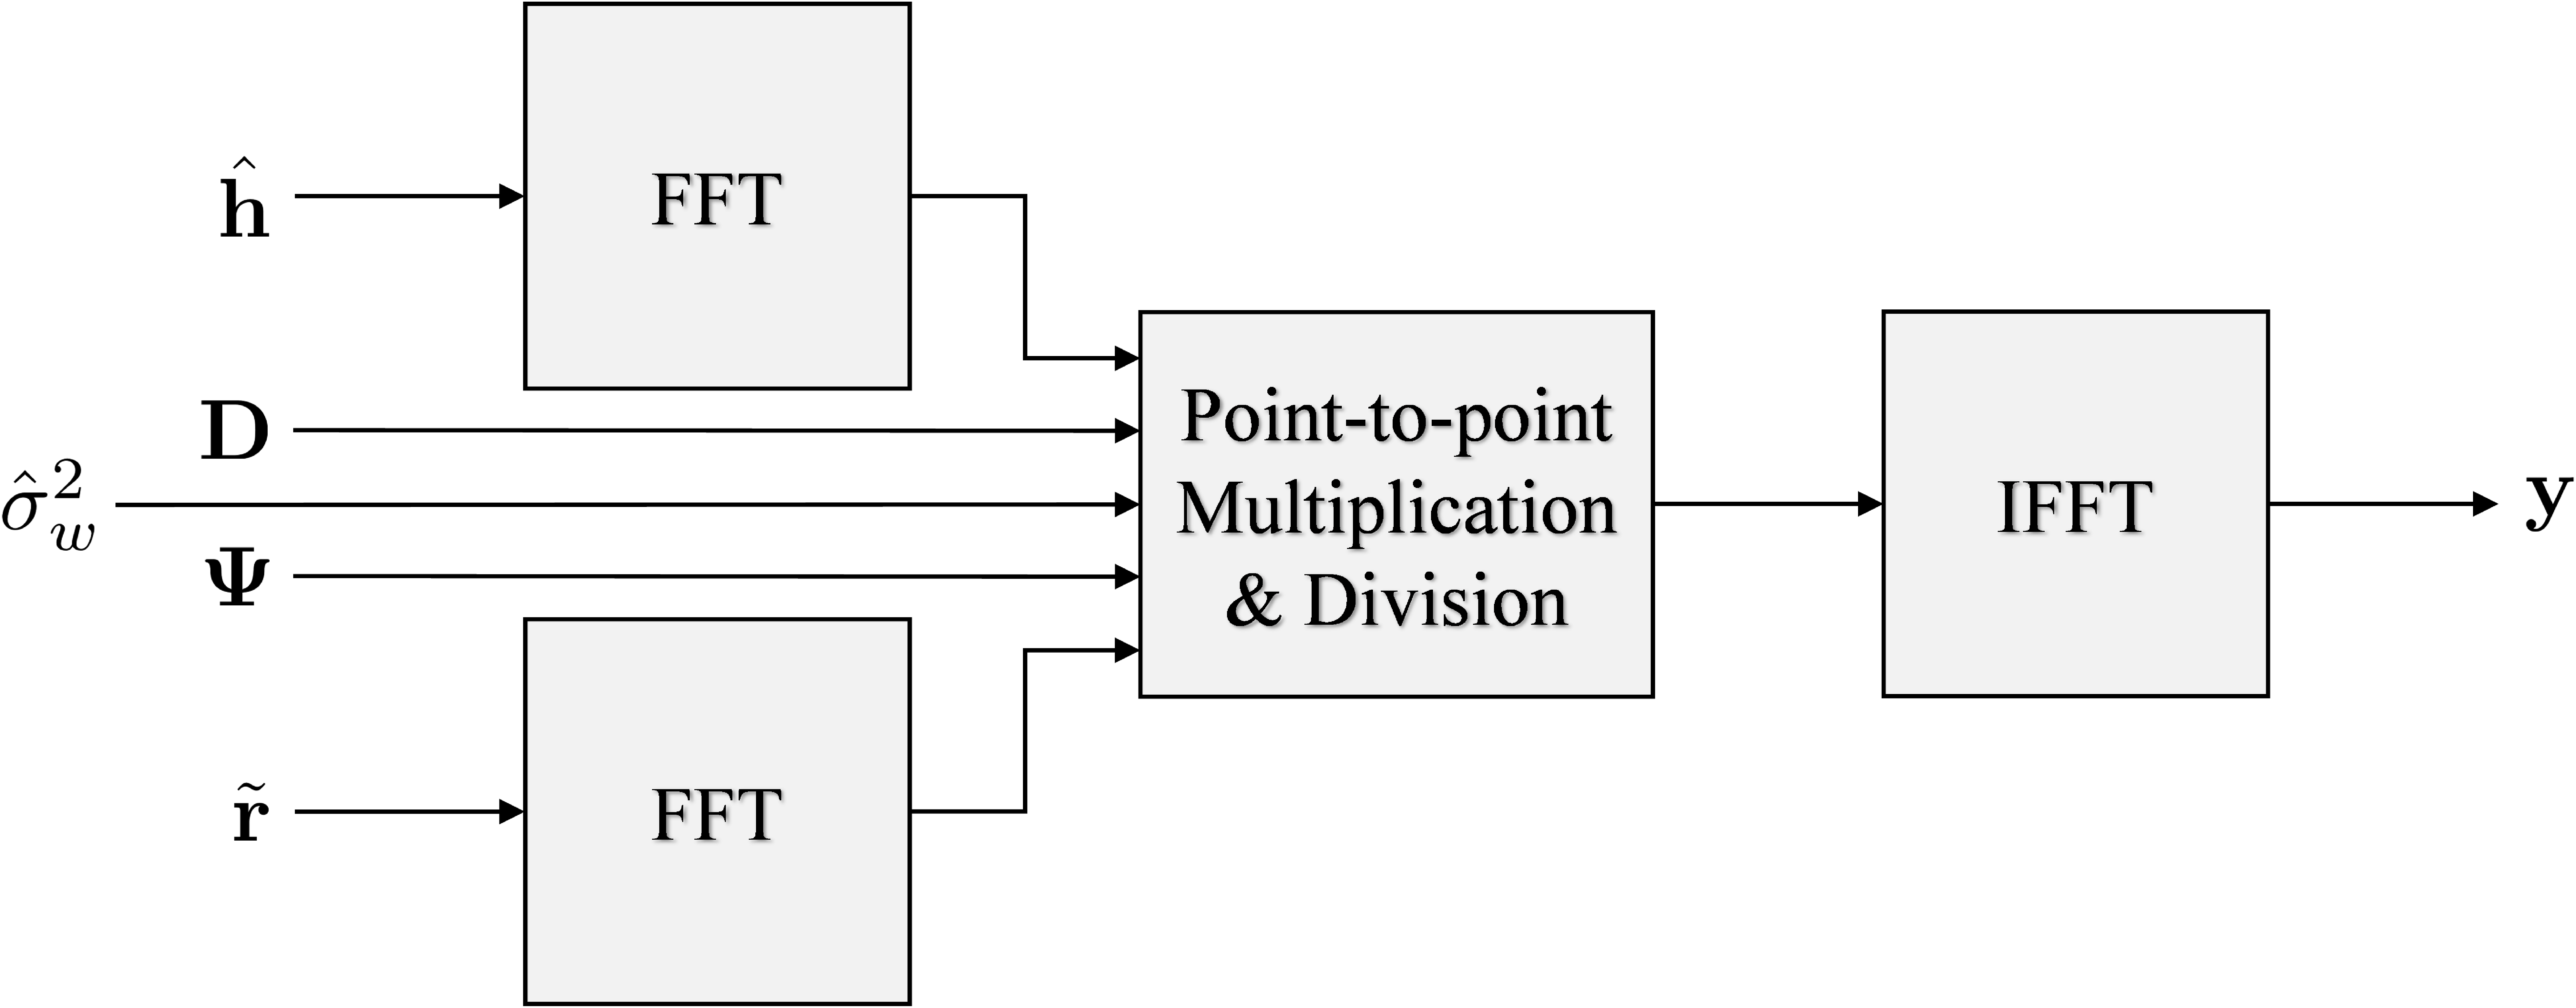
\includegraphics[width=10.03in/100*55]{figures/eq_GPUimplementation/blockFDE2.pdf}
	\caption{Diagram showing Frequency Domain Equalizer Two is implemented in the frequency domain in GPUs.}
	\label{fig:blockFDE2}
\end{figure}






\chapter{Summary and Conclusions}
\label{chap:final_summary}
\section{GPU Implementation}
Based on measured execution times of GPU kernels, multiple data-aided equalization filters where implemented for the purpose of equalizing an aeronautical telemetry channel.
Using GPU libraries and batch processing rather than custom designed GPU kernels produced massive speed ups.
Also, reformulating algorithms into frequency-domain convolution produced impressive speed ups.

For implementation in one Tesla K40c and two Tesla K20c GPUs the execution times for all equalizers met the real-time constraint.
It was shown that the frequency-domain equalizers are the easiest to implement and have the fastest execution time.
The CMA equalizer was shown to be the hardest to implement and has the slowest execution time.
The execution time did not provide the CMA the opportunity to iterate many times.
The ZF and MMSE equalizers were shown to be computationally challenging to implement but had an acceptable execution time.

Because data-aided equalizers are implemented for a real-time telemetry receiver system,
the execution time results must be considered along with the bit error rate performance.
%Despite the performance of the CMA equalizer in AWGN, the execution time per iteration does not allow the equalizer to converge in multipath.
As of this writing the FDE1 equalizer is recommended, marking the best tradeoff between performance and computational complexity.

\section{Contributions}
Through the years of working on the PAQ project I:
\begin{enumerate}
\item Implemented algorithms using batch GPU libraries to reduce execution time on average by 5.
\item Reduced GPU convolution time by using batch GPU librarys and cascading filters in the frequency domain.
\item Implemented linear solver libraries to make ZF and MMSE equalizers feasible and real-time.
\item Reformulated the CMA to leverage the speed of GPU convolution.
\item Implemented new ADC to drive success of the PAQ project.
\item Implemented resampling polyphase filters in GPUs.
\item Participated heavily in flight tests at Edwards AFB.
\item Presented a paper frequency offset compensation for equalized SOQPSK at International \newline Telemetering. Conference (ITC) \cite{ravert2016}.
\end{enumerate}

\section{Further Work}
The Levinson-Durbin algorithm GPU implementation only leveraged the toeplitz structure of the channel estimate auto-correlation matrix.
A hybrid sparse Levinson-Durbin algorithm could leverage the sparseness of the channel estimate auto-correlation matrix and the vector $\hat{\mathbf{h}}_{n_0}$.




%%%%%%%%%%%%% begin Bibliography %%%%%%%%%%%%%%%%%
\phantomsection %Forces a new section prior to setting the bibliography reference point
\bibliographystyle{IEEEtran}
\addcontentsline{toc}{chapter}{Bibliography}
\bibliography{refs}

% Bibliographies are best created and maintained using BibTeX
% To use Bibtex, create a bibliography file, e.g., refs.bib
% The sample file sources.bib shows examples of different
% bibliographic entries.
% The bibliography is created by executing:
%  1.  latex, 2. bibtex, 3. latex, 4. latex
%%%%%%%%%%%%%%%% end Bibliography %%%%%%%%%%%%%%%%%

%Included because WinEdit is RETARDED and it needs it for Gather Purposes:
%input "refs.bib"


% Include appendix sections here:
% each appendix should be a file with a .tex extension and the text
% of the file should begin with \appendix{Appendix Title}, followed
% by the contents of the appendix
%\appendix{Sample Appendix}

\section{Width Based on Page Size Figure Example} \label{sec:appendxia_figure_example}
Here's an example of a figure whose width depends on the width
of the page. You can see if as Figure \ref{fig:appendix_some_pic}.

\begin{figure}[htbp]
  \centering
  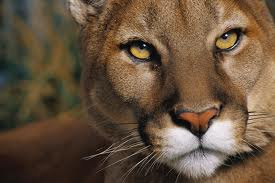
\includegraphics[width=0.45\textwidth]{figures/appendixa/some_pic}
  \caption[Example Width Based on Page Size Figure]{
    This is an example of a figure whose width will be 45\% of the
    width of the page. If you'd like to see a figure with a fixed
    width then you can see it as Figure \ref{fig:intro_stuff} in
    Section \ref{sec:intro_figure_example}. Just FYI, I made this
    figure with PowerPoint and then copied it and pasted it into
    wmf2eps and choose the "Paste EMF" option. It will generate
    a larger file, but it will look a TON better than the
    "Paste WMF" option and the "Paste DIB" option will paste the
    rasterized image that won't scale well at all.}
  \label{fig:appendix_some_pic}
\end{figure}

%End the document
\end{document}
